%% For double-blind review submission, w/o CCS and ACM Reference (max submission space)
%\documentclass[sigplan,10pt,review,anonymous]{acmart}
%\settopmatter{printfolios=false,printccs=false,printacmref=false}
%% For double-blind review submission, w/ CCS and ACM Reference
%\documentclass[sigplan,review,anonymous]{acmart}\settopmatter{printfolios=true}
%% For single-blind review submission, w/o CCS and ACM Reference (max submission space)
%\documentclass[sigplan,review]{acmart}\settopmatter{printfolios=true,printccs=false,printacmref=false}
%% For single-blind review submission, w/ CCS and ACM Reference
%\documentclass[sigplan,review]{acmart}\settopmatter{printfolios=true}
%% For final camera-ready submission, w/ required CCS and ACM Reference
%\documentclass[sigplan,nonacm]{acmart}
\documentclass[sigplan,review,anonymous,acmsmall]{acmart}\settopmatter{printfolios=false,printccs=false,printacmref=false}


%% Conference information
%% Supplied to authors by publisher for camera-ready submission;
%% use defaults for review submission.
\acmConference[SPLASH'23]{ACM SIGPLAN conference on Systems, Programming, Languages, and Applications: Software for Humanity}{October 22-27, 2023}{Cascais, Portugal}
%\acmYear{2018}
%\acmISBN{} % \acmISBN{978-x-xxxx-xxxx-x/YY/MM}
%\acmDOI{} % \acmDOI{10.1145/nnnnnnn.nnnnnnn}
%\startPage{1}

%% Copyright information
%% Supplied to authors (based on authors' rights management selection;
%% see authors.acm.org) by publisher for camera-ready submission;
%% use 'none' for review submission.
\setcopyright{none}
%\setcopyright{acmcopyright}
%\setcopyright{acmlicensed}
%\setcopyright{rightsretained}
%\copyrightyear{2018}           %% If different from \acmYear

%% Bibliography style
\bibliographystyle{acmart}

\usepackage{dsfont}
\usepackage{stmaryrd}
\usepackage{colortbl}
\usepackage{hyperref}

\usepackage{amsmath}
\DeclareMathOperator*{\argmax}{argmax}
\DeclareMathOperator*{\argmin}{argmin}
\usepackage{amssymb}

\usepackage[dvipsnames, table]{xcolor}
\usepackage{textcomp}

% Packages
\usepackage[pdf]{graphviz}
\usepackage{mathrsfs}

\newcommand*\circled[1]{\tikz[baseline=-0.1cm]{
  \node[shape=circle,draw,inner sep=0.48pt] (char) {\fontsize{7}{12}\textsf{#1}};}}

\DeclareMathAlphabet{\mathcal}{OMS}{cmsy}{m}{n}
\usepackage{cancel}
\newcommand\ccancel[2][red]{\renewcommand\CancelColor{\color{#1}}\cancel{#2}}
\newcommand{\nDownarrow}{\ensuremath{\text{ }\cancel{\Downarrow}\text{ }}}
\usepackage{centernot}

\usepackage{pgfplots, pgfplotstable}
\pgfplotsset{compat=1.7}
\usepgfplotslibrary{fillbetween}
\usetikzlibrary{patterns}
\pgfmathdeclarefunction{gauss}{2}{\pgfmathparse{1/(#2*sqrt(2*pi))*exp(-((x-#1)^2)/(2*#2^2))}}
\pgfmathdeclarefunction{nil}{1}{\pgfmathparse{0.001}}

\usepackage{arydshln}
\usepackage{adjustbox}
\usepackage{enumerate}
\usepackage{enumitem}
\usepackage{tikz-cd}
\usetikzlibrary{calc}
\usepackage{amsfonts}
%\usepackage{prooftrees}
\usepackage{bussproofs}
\renewcommand{\sectionautorefname}{\S}
\renewcommand{\subsectionautorefname}{\S}
\usepackage{float}

\usepackage{tikz-3dplot}
\usetikzlibrary{3d}
\usetikzlibrary{calligraphy}
\newif\ifshowcellnumber
\showcellnumbertrue

\usepackage{algorithm}
\usepackage{algpseudocode}
\usepackage{algorithmicx}
\usepackage{sourcecodepro}
\usepackage{tikz-qtree}
\usepackage{amsthm}
\usepackage{bm}
\usetikzlibrary{bayesnet}
\usetikzlibrary{arrows}
\usepackage{subcaption}
\usetikzlibrary{backgrounds}
\usetikzlibrary{tikzmark}

\newcommand{\E}{\mathbb{E}}
\newcommand{\Var}{\mathrm{Var}}
\newcommand{\Cov}{\mathrm{Cov}}

\newcommand{\CompOrder}{\mathcal{O}}
\def\graphspace{\mathbf{G}}
\def\Uniform{\mbox{\rm Uniform}}
\def\Gaussian{\mbox{\rm Gaussian}}
\def\Bernoulli{\mbox{\rm Bernoulli}}
\def\Dirichlet{\mbox{\rm Dirichlet}}

\usepackage{mathtools}% superior to amsmath
\usepackage{tikz}
% Packages
\usepackage{listings}
\DeclareRobustCommand{\hlred}[1]{{\sethlcolor{pink}\hl{#1}}}
\usepackage{fontspec}

\setmonofont[Scale=0.8]{JetBrainsMono}[
  Contextuals={Alternate},
  Path=./font/,
  Extension = .ttf,
  UprightFont=*-Regular,
  BoldFont=*-Bold,
  ItalicFont=*-Italic,
  BoldItalicFont=*-BoldItalic
]

\usepackage[skins,breakable,listings]{tcolorbox}

\lstdefinelanguage{kotlin}{
  comment=[l]{//},
  commentstyle={\color{gray}\ttfamily},
  emph={delegate, filter, firstOrNull, forEach, it, lazy, mapNotNull, println, repeat, assert, with, head, tail, len, return@},
  numberstyle=\noncopyable,
  identifierstyle=\color{black},
  keywords={abstract, actual, as, as?, break, by, class, companion, continue, data, do, dynamic, else, enum, expect, false, final, for, fun, get, if, import, in, infix, interface, internal, is, null, object, open, operator, override, package, private, public, return, sealed, set, super, suspend, this, throw, true, try, catch, typealias, val, var, vararg, when, where, while, tailrec, reified},
  keywordstyle={\bfseries},
  morecomment=[s]{/*}{*/},
  morestring=[b]",
  morestring=[s]{"""*}{*"""},
  ndkeywords={@Deprecated, @JvmField, @JvmName, @JvmOverloads, @JvmStatic, @JvmSynthetic, Array, Byte, Double, Float, Boolean, Int, Integer, Iterable, Long, Runnable, Short, String, int},
  ndkeywordstyle={\bfseries},
  sensitive=true,
  stringstyle={\ttfamily},
  literate={`}{{\char0}}1,
  escapeinside={(*@}{@*)}
}
\lstdefinelanguage{tidy}{
  comment=[l]{//},
  commentstyle={\color{gray}\ttfamily},
  emph={|, ->, ---},
  emphstyle={\color{red}},
  identifierstyle=\color{black},
  keywords={\|, ->, ---},
  otherkeywords={|,->},
  morekeywords={|,->},
  keywordstyle={\color{blue}\bfseries},
  morecomment=[s]{/*}{*/},
  morestring=[b]",
  morestring=[s]{"""*}{*"""},
  ndkeywords={@Deprecated, @JvmField, @JvmName, @JvmOverloads, @JvmStatic, @JvmSynthetic, Array, Byte, Double, Float, Int, Integer, Iterable, Long, Runnable, Short, String},
  ndkeywordstyle={\color{orange}\bfseries},
  sensitive=true,
  stringstyle={\color{green}\ttfamily},
  literate={`}{{\char0}}1
}

%%%%%%%%%%%%%%%%%%%%%%%%%%%%%%%%%%%%%%%%%%%
%
% Color boxes
%
%%%%%%%%%%%%%%%%%%%%%%%%%%%%%%%%%%%%%%%%%%%

\tcbset{
  enhanced jigsaw,
  breakable,
  listing only,
%  boxsep=-1pt,
%  top=-1pt,
  bottom=0.1cm,
  right=0.5cm,
  overlay first={
    \node[black!50] (S) at (frame.south) {\Large\ding{34}};
    \draw[dashed,black!50] (frame.south west) -- (S) -- (frame.south east);
  },
  overlay middle={
    \node[black!50] (S) at (frame.south) {\Large\ding{34}};
    \draw[dashed,black!50] (frame.south west) -- (S) -- (frame.south east);
    \node[black!50] (S) at (frame.north) {\Large\ding{34}};
    \draw[dashed,black!50] (frame.north west) -- (S) -- (frame.north east);
  },
  overlay last={
    \node[black!50] (S) at (frame.north) {\Large\ding{34}};
    \draw[dashed,black!50] (frame.north west) -- (S) -- (frame.north east);
  },
  before={\par\vspace{5pt}},
  after={\par\vspace{\parskip}\noindent}
}

\definecolor{slightgray}{rgb}{0.90, 0.90, 0.90}

\usepackage{soul}
\makeatletter
\def\SOUL@hlpreamble{%
  \setul{}{3.0ex}%
  \let\SOUL@stcolor\SOUL@hlcolor%
  \SOUL@stpreamble%
}
\makeatother

\newcommand{\inline}[1]{%
  \begingroup%
  \sethlcolor{slightgray}%
  \hl{\ttfamily\footnotesize #1}%
  \endgroup
}

\newcommand{\tinline}[1]{%
  \begingroup%
  \sethlcolor{slightgray}%
  \hl{\ttfamily\tiny #1}%
  \endgroup
}

\newtcblisting{halftidyinput}[1][]{%
  left skip=0.7cm,
  width=6cm,
%  left=-0.01cm,
  top=-0.1cm,
  bottom=-0.35cm,
  listing options={
    language=tidy,
    basicstyle=\ttfamily\small,
%numberstyle=\footnotesize,
    showstringspaces=false,
    tabsize=2,
    breaklines=true,
    numbers=none,
    inputencoding=utf8,
    escapeinside={(*@}{@*)},
    #1
  },
  underlay unbroken and first={%
    \path[draw=none] (interior.north west) rectangle node[white]{
\includegraphics[width=4mm]{../figures/tidyparse_logo.png}} ([xshift=-10mm,yshift=-7mm]interior.north west);
  }
}

\newtcblisting{wholetidyinput}[1][]{%
  left skip=0.7cm,
  top=0.1cm,
  middle=0mm,
  boxsep=0mm,
  listing options={
    language=tidy,
    basicstyle=\ttfamily\small,
%numberstyle=\footnotesize,
    showstringspaces=false,
    tabsize=2,
    breaklines=true,
    numbers=none,
    inputencoding=utf8,
    escapeinside={(*@}{@*)},
    #1
  },
  underlay unbroken and first={%
      \path[draw=none] (interior.north west) rectangle node[white]{
\includegraphics[width=4mm]{../figures/tidyparse_logo.png}} ([xshift=-10mm,yshift=-9mm]interior.north west);
  }
}

\definecolor{A}{RGB}{6,150,104}
\definecolor{B}{RGB}{196,74,137}
\definecolor{C}{RGB}{117,237,133}
\definecolor{D}{RGB}{246,46,243}
\definecolor{E}{RGB}{89,162,12}
\definecolor{F}{RGB}{113,12,158}
\definecolor{G}{RGB}{191,205,142}
\definecolor{H}{RGB}{51,58,158}
\definecolor{I}{RGB}{244,212,3}
\definecolor{J}{RGB}{37,36,249}
\definecolor{K}{RGB}{253,165,71}
\definecolor{L}{RGB}{27,81,29}
\colorlet{LA}{A!30}
\colorlet{LB}{B!30}
\colorlet{LC}{C!30}
\colorlet{LD}{D!30}
\colorlet{LE}{E!30}
\colorlet{LF}{F!30}
\colorlet{LG}{G!30}
\colorlet{LH}{H!30}
\colorlet{LI}{I!30}
\colorlet{LJ}{J!30}
\colorlet{LK}{K!30}
\colorlet{LL}{L!30}
\newcommand{\hiliA}[1]{%
  \colorbox{LA}{$#1$}}
\newcommand{\hiliB}[1]{%
  \colorbox{LB}{$#1$}}
\newcommand{\hiliC}[1]{%
  \colorbox{LC}{$#1$}}
\newcommand{\hiliD}[1]{%
  \colorbox{LD}{$#1$}}
\newcommand{\hiliE}[1]{%
  \colorbox{LE}{$#1$}}
\newcommand{\hiliF}[1]{%
  \colorbox{LF}{$#1$}}
\newcommand{\hiliG}[1]{%
  \colorbox{LG}{$#1$}}
\newcommand{\hiliH}[1]{%
  \colorbox{LH}{$#1$}}
\newcommand{\hiliI}[1]{%
  \colorbox{LI}{$#1$}}
\newcommand{\hiliJ}[1]{%
  \colorbox{LJ}{$#1$}}
\newcommand{\hiliK}[1]{%
  \colorbox{LK}{$#1$}}
\newcommand{\hiliL}[1]{%
  \colorbox{LL}{$#1$}}
\newcommand{\highlight}[1]{%
  \colorbox{lgray}{$#1$}}
\colorlet{lred}{red!30}
\colorlet{lorange}{orange!30}
\colorlet{lgreen}{green!30}
\colorlet{lgray}{black!15}
\colorlet{dgray}{black!75}
\DeclareRobustCommand{\hlred}[1]{{\sethlcolor{lred}\hl{#1}}}
\DeclareRobustCommand{\hlorange}[1]{{\sethlcolor{lorange}\hl{#1}}}
\DeclareRobustCommand{\hlgreen}[1]{{\sethlcolor{lgreen}\hl{#1}}}
\DeclareRobustCommand{\hlgray}[1]{{\sethlcolor{lgray}\hl{#1}}}
\DeclareRobustCommand{\caret}[1]{{\sethlcolor{dgray}\textcolor{white}{\hl{#1}}}}

\usepackage{url}
\usepackage{qtree}

\usepackage{filecontents}
\usepackage{pstricks-add}
\usepackage{emoji}
\usepackage{alltt}
\usepackage{nicematrix}
\usepackage{graphicx}
\usepackage{ulem}
\usepackage{upquote}
\tikzstyle{every picture}+=[remember picture]
\usepackage{menukeys}
\pgfplotstableread[col sep=comma,]{timings_loc.csv}\loctimings
\pgfplotstableread[col sep=comma,]{timings_unloc.csv}\unloctimings

\makeatletter
\DeclareRobustCommand{\cev}[1]{%
  {\mathpalette\do@cev{#1}}%
}
\newcommand{\do@cev}[2]{%
  \vbox{\offinterlineskip
  \sbox\z@{$\m@th#1 x$}%
  \ialign{##\cr
  \hidewidth\reflectbox{$\m@th#1\vec{}\mkern4mu$}\hidewidth\cr
  \noalign{\kern-\ht\z@}
    $\m@th#1#2$\cr
  }%
  }%
}
\makeatother

\makeatletter
\DeclareRobustCommand{\pder}[1]{%
  \@ifnextchar\bgroup{\@pder{#1}}{\@pder{}{#1}}}
\newcommand{\@pder}[2]{\frac{\partial#1}{\partial#2}}
\makeatother

\newcommand{\shup}{\shortuparrow}
\newcommand{\shri}{\shortrightarrow}
\newcommand{\shur}{\shup\hspace{-5pt}\shri}

\makeatletter
\def\squiggly{\bgroup \markoverwith{\textcolor{red}{\lower3\p@\hbox{\sixly \char58}}}\ULon}
\makeatother

\newcommand{\err}[1]{\smash{\squiggly{#1}{}}}
\newcommand{\stirlingii}{\genfrac{\{}{\}}{0pt}{}}

%======== Arrows =========
\newcommand{\knightarrow}{
  \tikz{
    \fill (0pt,0pt) circle [radius = 1pt];
    \fill (0pt,6pt) circle [radius = 1pt];
    \fill (6pt,0pt) circle [radius = 1pt];
    \fill (6pt,6pt) circle [radius = 1pt];
    \fill (12pt,0pt) circle [radius = 1pt];
    \fill (12pt,6pt) circle [radius = 1pt];
    \fill (6pt,0pt) circle [radius = 1pt];
    \fill (12pt,0pt) circle [radius = 1pt];
    \draw [-to] (0pt,0pt) -- (12pt,6pt);
  }
}

\newcommand{\kingarrow}{
  \tikz{
    \fill (0pt,0pt) circle [radius = 1pt];
    \fill (6pt,0pt) circle [radius = 1pt];
    \fill (0pt,6pt) circle [radius = 1pt];
    \fill (6pt,6pt) circle [radius = 1pt];
    \draw [-to] (0pt,0pt) -- (6pt,6pt);
    \draw [-to] (0pt,0pt) -- (0pt,6pt);
    \draw [-to] (0pt,0pt) -- (6pt,0pt);
  }
}

\newcommand{\knightkingarrow}{
  \tikz{
    \fill (0pt,0pt) circle [radius = 1pt];
    \fill (0pt,6pt) circle [radius = 1pt];
    \fill (6pt,0pt) circle [radius = 1pt];
    \fill (6pt,6pt) circle [radius = 1pt];
    \fill (12pt,0pt) circle [radius = 1pt];
    \fill (12pt,6pt) circle [radius = 1pt];
    \draw [-to] (0pt,0pt) -- (6pt,6pt);
    \draw [-to] (0pt,0pt) -- (0pt,6pt);
    \draw [-to] (0pt,0pt) -- (6pt,0pt);
    \draw [-to] (0pt,0pt) -- (12pt,6pt);
  }
}

%======== Arrows =========

\usetikzlibrary{decorations.pathreplacing,automata,calc,positioning,matrix,fit}
\usepackage{wrapfig}

\newcommand{\mkTrellis}[1]{
  \begin{tikzpicture}
    \def\dx{20pt}
    \def\dy{30pt}
    \newcounter{i}
    \stepcounter{i}
    \node[circle, draw, fill=black!30] (\arabic{i}) at (0,0){};
    \foreach [count=\i] \x in {2,...,#1}{
      \pgfmathsetmacro{\lox}{\x-1}%
      \pgfmathsetmacro{\loxt}{\x-3}%
      \foreach [count=\j] \xx in {-\lox,-\loxt,...,\lox}{
        \pgfmathsetmacro{\jj}{\j-1}%
        \stepcounter{i}
        \pgfmathsetmacro{\kk}{\xx-2}%
        \pgfmathsetmacro{\lbl}{\lox!/(\jj!*(\lox-\jj)!)}
        \ifnum\x<\kk
        \pgfmath\node[circle, draw]  (\arabic{i}) at (\xx*\dx, -\lox*\dy) {};
        \else
        \pgfmath\node[circle, draw, fill=black!30]  (\arabic{i}) at (\xx*\dx, -\lox*\dy) {};
        \fi
      }
    }
    \newcounter{z}
    \newcounter{xn}
    \newcounter{xnn}
    \pgfmathsetmacro{\maxx}{#1 - 1}
    \foreach \x in {1,...,\maxx}{
      \foreach \xx in {1,...,\x}{
        \stepcounter{z}
        \setcounter{xn}{\arabic{z}}
        \addtocounter{xn}{\x}
        \setcounter{xnn}{\arabic{xn}}
        \stepcounter{xnn}
        \draw [<-] (\arabic{z}) -- (\arabic{xn});
        \draw [<-] (\arabic{z}) -- (\arabic{xnn});
      }
    }
  \end{tikzpicture}
}

\newcommand{\dx}{20pt}
\newcommand{\dy}{30pt}
\newcounter{i}
\newcounter{z}
\newcounter{xn}
\newcounter{xnn}
\newcommand{\mkTrellisAppend}[1]{
  \begin{tikzpicture}
    \setcounter{i}{0}
    \setcounter{z}{0}
    \setcounter{xn}{0}
    \setcounter{xnn}{0}
    \stepcounter{i}
    \node[circle, draw] (\arabic{i}) at (0,0){};
    \foreach [count=\i] \x in {2,...,#1}{
      \pgfmathsetmacro{\lox}{\x-1}%
      \pgfmathsetmacro{\loxt}{\x-3}%
      \foreach [count=\j] \xx in {-\lox,-\loxt,...,\lox}{
        \pgfmathsetmacro{\jj}{\j-1}%
        \stepcounter{i}
        \pgfmathsetmacro{\kk}{\xx+2}%
        \pgfmathsetmacro{\lbl}{\lox!/(\jj!*(\lox-\jj)!)}
        \ifnum\x>\kk
        \pgfmath\node[circle, draw, fill=black!30]  (\arabic{i}) at (\xx*\dx, -\lox*\dy) {};
        \else
        \pgfmath\node[circle, draw]  (\arabic{i}) at (\xx*\dx, -\lox*\dy) {};
        \fi
      }
    }
    \pgfmathsetmacro{\maxx}{#1 - 1}
    \foreach \x in {1,...,\maxx}{
      \foreach \xx in {1,...,\x}{
        \stepcounter{z}
        \setcounter{xn}{\arabic{z}}
        \addtocounter{xn}{\x}
        \setcounter{xnn}{\arabic{xn}}
        \stepcounter{xnn}
        \draw [<-] (\arabic{z}) -- (\arabic{xn});
        \draw [<-] (\arabic{z}) -- (\arabic{xnn});
      }
    }
  \end{tikzpicture}
}

\newcommand{\mkTrellisInsert}[1]{
  \begin{tikzpicture}
    \setcounter{i}{0}
    \setcounter{z}{0}
    \setcounter{xn}{0}
    \setcounter{xnn}{0}
    \stepcounter{i}
    \node[circle, draw] (\arabic{i}) at (0,0){};
    \foreach [count=\i] \x in {2,...,#1}{
      \pgfmathsetmacro{\lox}{\x-1}%
      \pgfmathsetmacro{\loxt}{\x-3}%
      \foreach [count=\j] \xx in {-\lox,-\loxt,...,\lox}{
        \pgfmathsetmacro{\jj}{\j-1}%
        \stepcounter{i}
        \pgfmathsetmacro{\mp}{\xx+#1}%
        \pgfmathsetmacro{\mq}{\xx+\x}%
        \pgfmathsetmacro{\lbl}{\lox!/(\jj!*(\lox-\jj)!)}
        \ifnum\x>\mp
        \pgfmath\node[circle, draw, fill=black!30]  (\arabic{i}) at (\xx*\dx, -\lox*\dy) {};
        \else
        \ifnum#1<\mq
        \pgfmath\node[circle, draw, fill=black!30]  (\arabic{i}) at (\xx*\dx, -\lox*\dy) {};
        \else
        \pgfmath\node[circle, draw]  (\arabic{i}) at (\xx*\dx, -\lox*\dy) {};
        \fi
        \fi

      }
    }
    \pgfmathsetmacro{\maxx}{#1 - 1}
    \foreach \x in {1,...,\maxx}{
      \foreach \xx in {1,...,\x}{
        \stepcounter{z}
        \setcounter{xn}{\arabic{z}}
        \addtocounter{xn}{\x}
        \setcounter{xnn}{\arabic{xn}}
        \stepcounter{xnn}
        \draw [<-] (\arabic{z}) -- (\arabic{xn});
        \draw [<-] (\arabic{z}) -- (\arabic{xnn});
      }
    }
  \end{tikzpicture}
}

\usetikzlibrary{automata, positioning, arrows}

\newcommand{\nobarfrac}{\genfrac{}{}{0pt}{}}
\pgfplotstableread[col sep=comma,]{timings_loc.csv}\loctimings
\pgfplotstableread[col sep=comma,]{timings_unloc.csv}\unloctimings
\pgfplotstableread[col sep=comma,]{natural_errors.csv}\naturalerrors
\pgfplotstableread[col sep=comma,]{synthetic_errors.csv}\syntheticerrors

\begin{document}

%% Title information
\title{Syntax Error Correction as Idempotent Matrix Completion}
\begin{abstract}
In this work, we illustrate how to lower context-free language recognition onto a tensor algebra over finite fields. In addition to its theoretical value, this connection has yielded surprisingly useful applications in incremental parsing, code completion and program repair. For example, we use it to repair syntax errors, perform sketch-based program synthesis, and decide various language induction and membership queries. This line of research provides an elegant unification of context-free program repair, code completion and sketch-based program synthesis. To accelerate code completion, we design and implement a novel incremental parser-synthesizer that transforms CFGs onto a dynamical system over finite field arithmetic, enabling us to suggest syntax repairs in-between keystrokes.
\end{abstract}

\maketitle

\section{Introduction}

Syntax correction is one of the first problems that novice programmers encounter when learning to write code and a persistent issue in computer programming. Put simply, it is the problem of editing a syntactically incorrect program fragment so that it parses. This problem is particularly challenging because not only are programming languages syntactically context-sensitive, increasing the search space exponentially, but also because of the highly under-determined structure of the solution: repairs must make sense in the context of the surrounding code, and the correct repair is seldom unique, even assuming minimality.

Most prior work in syntax correction is a combination of two approaches: (1) \textit{pattern matching}, which uses hand-crafted rules to identify and correct common syntax errors, and (2) \textit{machine learning}, which trains a model to edit code. The former approach is effective in certain scenarios, but limited by the number of rules, while the latter approach is more general, but requires a large amount of training data, which is often unavailable in practice and generalizes poorly under distributional shift.

In this paper, we present a new approach to syntax correction, which unifies code completion, syntax correction, and program repair. Our approach shares connections to \textit{language reachability}, \textit{array programming} and \textit{tensor completion}. We show how the problem of syntax correction can be recast as a special case of tensor completion, enabling parallelization and integrating smoothly into both machine learning and contraint propagation. We show this approach scales to solve real-world program repair scenarios, and implement it in a real-time editor called Tidyparse.

\section{Background}

The great compromise in program synthesis is one of efficiency versus expressiveness: the more expressive a language, the more concise and varied the programs it can represent, but the harder those programs are to synthesize without resorting to domain-specific heuristics. Likewise, the simpler a language is to synthesize, the weaker its concision and expressive power.

Most existing work on program synthesis focus on general $\lambda$-calculi, or very narrow languages such as finite automata or regular expressions. The former are too expressive to be synthesized or verified, whilst the latter are too restrictive to be useful. In our work, we focus on context-free and mildly context-sensitive grammars, which are expressive enough to capture a variety of useful programming language features, but not so expressive as to be unsynthesizable.

The second great compromise in program synthesis is that of reusability versus specialization. In programming, as in human affairs, there is a vast constellation of languages, each requiring specialized generators and interpreters. Are these languages truly irreconcilable? Or, as Noam Chomsky argues, are these merely dialects of a universal language? \textit{Synthesis} then, might be a misnomer, and more aptly called \textit{recognition}, in the analytic tradition.

In our work, we argue these two compromises are not mutually exclusive, but complementary and reciprocal. Programs and the languages they inhabit are indeed synthetic, but can be analyzed and reused in the metalanguage of context-free grammars closed under conjunction. Not only does this admit an efficient synthesis algorithm, but allows users to introduce additional constraints without breaking compositionality, one of the most sacred tenets in programming language design.

Furthermore, we argue it is possible to improve the efficiency of human programmers without sacrificing expressiveness by considering latency to synthesize an acceptable completion. In contrast with program synthesizers that require intermediate programs to be well-formed, our synthesizer is provably sound and complete up to a Levenshtein distance bound, and attempts to minimize total edits, but does not impose any constraints on the code itself being written.


\section{Toy Example}

Suppose we are given the following context-free grammar:

\begin{wholetidyinput}
S -> S and S | S xor S | ( S ) | true | false | ! S(*@\caret{ }@*)
\end{wholetidyinput}

\noindent For reasons that will become clear in Sec.~\ref{sec:matrix}, this will automatically be rewritten into the grammar:

\begin{verbatim}
 F.! → !     S.) → S F.)  and.S → F.and S   S → F.! S     S → false    S → S ε+
 F.( → (   F.xor → xor    xor.S → F.xor S   S → S and.S   S → true    ε+ → ε
 F.) → )   F.and → and        S → S xor.S   S → F.( S.)   S → <S>     ε+ → ε+ ε+
\end{verbatim}

%\noindent We can visualize the CFG as either a graph or a matrix:
%
%\begin{figure}[H]
%    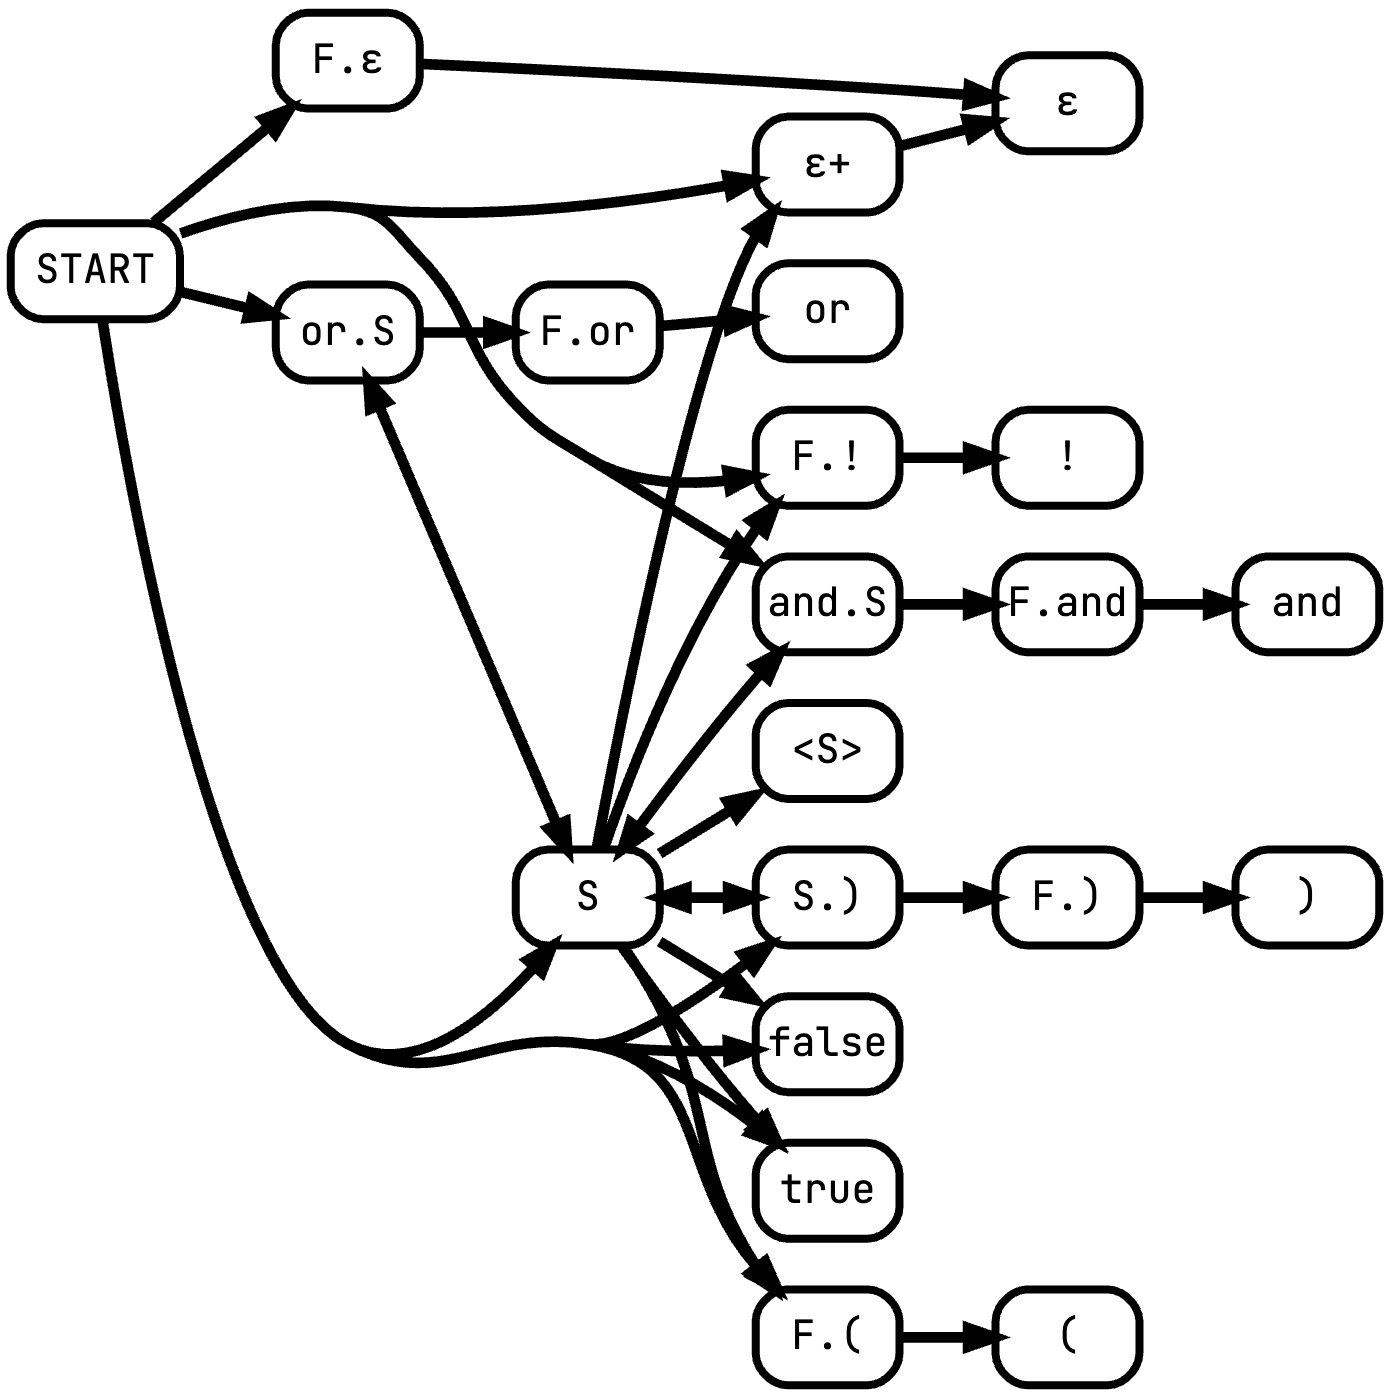
\includegraphics[width=3.5cm]{../figures/bool_arith_cfg_graph.png}
%    \hspace{20pt}
%    \includegraphics[width=3.5cm]{../figures/bool_arith_cfg_mat.bmp}
%\end{figure}

\noindent Given a string containing holes, our tool will return several completions in a few milliseconds:

\begin{tcolorbox}[left skip=0.7cm,
top=0.1cm,
middle=0mm,
boxsep=0mm,
underlay unbroken and first={%
    \path[draw=none] (interior.north west) rectangle node[white]{
\includegraphics[width=4mm]{../figures/tidyparse_logo.png}} ([xshift=-10mm,yshift=-9mm]interior.north west);
}]
  \begin{lstlisting} [language=tidy, basicstyle=\ttfamily\small, escapeinside={(*@}{@*)}]
true _ _ _ ( false _ ( _ _ _ _ ! _ _ ) _ _ _ _(*@\caret{ }@*)
  \end{lstlisting}
  \tcblower
  \begin{lstlisting} [language=tidy, basicstyle=\ttfamily\small, escapeinside={(*@}{@*)}]
true (*@\hlorange{xor}@*) (*@\hlorange{!}@*) ( false (*@\hlorange{xor}@*) ( <S> (*@\hlorange{)}@*) or ! (*@\hlorange{<S>}@*) ) (*@\hlorange{xor}@*) (*@\hlorange{<S>}@*)
true (*@\hlorange{xor}@*) (*@\hlorange{!}@*) ( false (*@\hlorange{and}@*) ( <S> (*@\hlorange{)}@*) or ! (*@\hlorange{<S>}@*) ) (*@\hlorange{xor}@*) (*@\hlorange{<S>}@*)
true (*@\hlorange{xor}@*) (*@\hlorange{!}@*) ( false (*@\hlorange{and}@*) ( <S> (*@\hlorange{)}@*) and ! (*@\hlorange{<S>}@*) ) (*@\hlorange{xor}@*) (*@\hlorange{<S>}@*)
true (*@\hlorange{xor}@*) (*@\hlorange{!}@*) ( false (*@\hlorange{and}@*) ( <S> (*@\hlorange{)}@*) and ! (*@\hlorange{<S>}@*) ) (*@\hlorange{and}@*) (*@\hlorange{<S>}@*)
...
  \end{lstlisting}
\end{tcolorbox}

\noindent Similarly, if provided with a string containing various errors, it will return several suggestions how to fix it, where \hlgreen{green} is insertion, \hlorange{orange} is substitution and \hlred{red} is deletion.

\begin{tcolorbox}[left skip=0.7cm,
top=0.1cm,
middle=0mm,
boxsep=0mm,
underlay unbroken and first={%
    \path[draw=none] (interior.north west) rectangle node[white]{
\includegraphics[width=4mm]{../figures/tidyparse_logo.png}} ([xshift=-10mm,yshift=-9mm]interior.north west);
}]
\begin{lstlisting} [language=tidy, basicstyle=\ttfamily\small, escapeinside={(*@}{@*)}]
true and ( false or and true false(*@\caret{ }@*)
\end{lstlisting}
\tcblower
\begin{lstlisting} [language=tidy, basicstyle=\ttfamily\small, escapeinside={(*@}{@*)}]
1.) true and ( false or (*@\hlorange{!}@*) true (*@\hlorange{)}@*)
2.) true and ( false or (*@\hlgreen{<S>}@*) and true (*@\hlorange{)}@*)
3.) true and ( false or (*@\hlorange{(}@*) true (*@\hlorange{)}@*) (*@\hlgreen{)}@*)
...
9.) true and ( false or (*@\hlgreen{!}@*) (*@\hlgreen{<S>}@*) (*@\hlgreen{)}@*) and true (*@\hlred{false} @*)
\end{lstlisting}
\end{tcolorbox}

\noindent In the following paper, we will describe how we built it.

\section{Matrix Theory}\label{sec:matrix}

Recall that a CFG is a quadruple consisting of terminals $(\Sigma)$, nonterminals $(V)$, productions $(P\colon V \rightarrow (V \mid \Sigma)^*)$, and a start symbol, $(S)$. It is a well-known fact that every CFG is reducible to \textit{Chomsky Normal Form}, $P'\colon V \rightarrow (V^2 \mid \Sigma)$, in which every production takes one of two forms, either $w \rightarrow xz$, or $w \rightarrow t$, where $w, x, z: V$ and $t: \Sigma$. For example:\vspace{-3pt}

\begin{table}[H]
\begin{tabular}{llll}
$\mathcal{G}:=\big\{\;S \rightarrow S\:S \mid (\:S\:) \mid (\:)\;\big\} \Longrightarrow \mathcal{G}'=\big\{\;S\rightarrow Q\:R \mid S\:S \mid L\:R,$ & $R \rightarrow\:),$ & $L \rightarrow (,$ & $Q\rightarrow L\:S\;\big\}$
\end{tabular}
\end{table}\vspace{-8pt}

\noindent Given a CFG, $\mathcal{G}' : \mathbb{G} = \langle \Sigma, V, P, S\rangle$ in CNF, we can construct a recognizer $R: \mathbb{G} \rightarrow \Sigma^n \rightarrow \mathbb{B}$ for strings $\sigma: \Sigma^n$ as follows. Let $2^V$ be our domain, $0$ be $\varnothing$, $\oplus$ be $\cup$, and $\otimes$ be defined as:\vspace{-10pt}

\begin{align}
X \otimes Z := \big\{\;w \mid \langle x, z\rangle \in X \times Z, (w\rightarrow xz) \in P\;\big\}
\end{align}

\noindent If we define $\sigma_r^{\shur} \coloneqq \{w \mid (w \rightarrow \sigma_r) \in P\}$, then construct a matrix with nonterminals on the superdiagonal representing each token, $M^0_{r+1=c}(\mathcal{G}', e) := \;\sigma_r^{\shur}$ and solve for the fixpoint $M^* = M + M^2$,\vspace{-10pt}

\begin{align*}
M^0:=
\begin{pNiceMatrix}[nullify-dots,xdots/line-style=loosely dotted]
   \varnothing & \sigma_1^\shri & \varnothing & \Cdots & \varnothing \\
   \Vdots      & \Ddots         & \Ddots      & \Ddots & \Vdots\\
               &                &             &        & \varnothing\\
               &                &             &        & \sigma_n^\shup \\
   \varnothing & \Cdots         &             &        & \varnothing
\end{pNiceMatrix} &\Rightarrow
\begin{pNiceMatrix}[nullify-dots,xdots/line-style=loosely dotted]
  \varnothing & \sigma_1^\shri & \Lambda & \Cdots & \varnothing \\
  \Vdots      & \Ddots         & \Ddots  & \Ddots & \Vdots\\
              &                &         &        & \Lambda\\
              &                &         &        & \sigma_n^\shup \\
  \varnothing & \Cdots         &         &        & \varnothing
\end{pNiceMatrix} &\Rightarrow \ldots \Rightarrow M^* =
\begin{pNiceMatrix}[nullify-dots,xdots/line-style=loosely dotted]
   \varnothing & \sigma_1^\shri & \Lambda & \Cdots & \Lambda^*_\sigma\\
   \Vdots      & \Ddots         & \Ddots  & \Ddots & \Vdots\\
               &                &         &        & \Lambda\\
               &                &         &        & \sigma_n^\shup \\
   \varnothing & \Cdots         &         &        & \varnothing
\end{pNiceMatrix}
\end{align*}

\noindent we obtain the recognizer, $R(\mathcal{G}', \sigma) := S \in \Lambda^*_\sigma? \Leftrightarrow \sigma \in \mathcal{L}(\mathcal{G})?$

Since $\bigoplus_{c = 1}^n M_{r,c} \otimes M_{c,r}$ has cardinality bounded by $|V|$, it can be represented as $\mathbb{Z}_2^{|V|}$ using the characteristic function, $\mathds{1}$. Note that any encoding which respects linearity $\varphi(\Lambda \circledast \Lambda') \equiv \varphi(\Lambda) \circledast \varphi(\Lambda')$ is suitable -- this particular representation shares the same algebraic structure, but is more widely studied in error correction, and readily compiled into circuits and BLAS primitives. Furthermore, it enjoys the benefit of complexity-theoretic speedups to matrix multiplication.

Details of the bisimilarity between parsing and matrix multiplication can be found in Valiant~\cite{valiant1975general}, who first realized its time complexity was subcubic $\mathcal{O}(n^\omega)$ where $\omega$ is the asymptotic lower bound for Boolean matrix multiplication ($\omega < 2.77$), and Lee~\cite{lee2002fast}, who shows that speedups to CFL parsing were realizable by Boolean matrix multiplication algorithms. While more efficient specialized parsers are known to exist for restricted CFGs, this technique is typically lineararithmic under sparsity and believed to be the most efficient general procedure for CFL parsing.

Valiant's decision procedure can be abstracted by lifting into the domain of bitvector variables, i.e., linear equations over finite fields, where each nonterminal inhabitant of the northeasternmost bitvector $\mathcal{T}$ will instead become an algebraic expression whose solutions correspond to valid parse forests for an incomplete string on the superdiagonal. This yields a novel interpretation of Valiant's algorithm as an equational theory over finite fields, allowing us to solve for admissible completions and their parse forests. In particular, $\boxplus$ and $\boxtimes$ are defined so the following diagram commutes,\footnote{Hereinafter, we use gray highlighting to denote types and functions defined over strings and binary constants only.}

\begin{figure}[H]
  \adjustbox{center}{%
    \[\begin{tikzcd}[row sep=large, column sep=huge]
        \langle\mathcal{G}', \highlight{\Sigma}^{n-1}\rangle \arrow[leftrightarrow, drrr, shorten=-1mm] & & [-135pt] & \vspace{20pt}\stackrel{\text{(Parsing)}}{\text{Set}} \arrow[d, phantom] & \stackrel{\text{(Recognition)}}{\text{Bit}} \arrow[d, phantom] & [-90pt] & \langle\mathcal{G}', \Sigma^{n-1}\rangle \arrow[drr, shorten=-2mm] & [-90pt] & \stackrel{\text{(Synthesis)}}{\text{SAT}} \arrow[d, phantom]\\[-30pt]
        \text{Rubix}  \arrow[rr, phantom] & & [-135pt] & M \times M \arrow[r, "\mathds{1}^{2^{n\times n}}", labels=above] \arrow[d, "\hspace{-13pt}\bigoplus\:\bigotimes"] & \mathbb{Z}_2^{|V|^{n\times n}} \times \mathbb{Z}_2^{|V|^{n\times n}} \arrow[d, "\hspace{-13.4pt}\highlight{+}\:\highlight{*}"] \arrow[l, "\mathds{1}^{-2^{n\times n}}", labels=below] \arrow[rrrr, rightarrowtail, "\varphi^{2^{n\times n}}", labels=above] & [-90pt] & & [-90pt] & \mathcal{M} \times \mathcal{M} \arrow[llll, rightharpoonup, shorten=1mm, "\varphi^{-2^{n\times n}}", labels=below] \arrow[d, "\hspace{-9pt}+\:\:\:*"] \\
        \text{Matrix} \arrow[rr, phantom] & & [-135pt] & 2^V \times 2^V \arrow[r, "\mathds{1}^{2}", labels=above] \arrow[d, "\hspace{-9pt}\oplus\:\otimes"] & \mathbb{Z}_2^{|V|} \times \mathbb{Z}_2^{|V|} \arrow[d, "\hspace{-15.8pt}\highlight{\boxplus}\:\highlight{\boxtimes}"] \arrow[l, "\mathds{1}^{-2}", labels=below] \arrow[rrrr, rightarrowtail, "\varphi^2", labels=above] & [-90pt] & & [-90pt] & \mathcal{V} \times \mathcal{V} \arrow[llll, rightharpoonup, shorten=1mm, "\varphi^{-2}", labels=below] \arrow[d, "\hspace{-9.5pt}\boxplus\:\boxtimes"] \arrow[u] \\
        \text{Vector} \arrow[rr, phantom] & & [-135pt] & 2^V \arrow[r, "\mathds{1}", labels=above] & \mathbb{Z}_2^{|V|} \arrow[l, "\mathds{1}^{-1}", labels=below] \arrow[rrrr, rightarrowtail, "\varphi", labels=above] & [-90pt] & & [-90pt] & \mathcal{V} \arrow[llll, rightharpoonup, shorten=1mm, "\varphi^{-1}", labels=below] \arrow[u]
    \end{tikzcd}\]
  }
\end{figure}

\noindent where $\mathcal{V}$ is a function $\mathbb{Z}_2^{|V|}\rightarrow\mathbb{Z}_2$. Note that while always possible to encode $\mathbb{Z}_2^{|V|} \rightarrow \mathcal{V}$ using the identity function, an arbitrary $\mathcal{V}$ might have zero, one, or in general, multiple solutions in $\mathbb{Z}_2^{|V|}$. In practice, this means that a language equation can be unsatisfiable or underconstrained, however if a solution exists, it can always be decoded into a valid sentence and parse forest in the language.

So far, we have only considered the syntactic theory of breadth-bounded CFLs with holes, however, our construction can be easily extended to handle the family of CFLs closed under conjunction. The additional expressivity afforded by the language conjunction operator will be indispensable when considering practical program repair scenarios, which may require extra-grammatical constraints such as indentation-sensitivity or Levenshtein-bounded reachability. That extension, and the resulting theory of breadth-bounded CJLs with holes, will be explored in Sec.~\ref{sec:lclreach}.

\section{Tree Denormalization}

% https://www.ling.upenn.edu/advice/latex/qtree/qtreenotes.pdf
% https://cpb-us-w2.wpmucdn.com/campuspress.yale.edu/dist/0/119/files/2014/12/sec-10.17-drawing-arrows-2ek9r2b.pdf

Our parser emits a binary forest consisting of parse trees for the candidate string which are constructed bottom-up using a variant of $\otimes$ called $\hat{\otimes}$, which simply records backpointers:

\begin{align}
   X\:\hat{\otimes}\:Z := \big\{\;w\hphantom{.}^{\nearrow}_{\searrow}\nobarfrac{x}{z} \mid \langle x, z\rangle \in X \times Z, (w\rightarrow xz) \in P\;\big\}
\end{align}

Due to Chomsky normalization however, the resulting forests are full of trees that are thin and crooked. To restore the natural shape of the tree, we first construct the parse forests bottom-up, then prune away synthetic nonterminals top-down by recursively grafting denormalized grandchildren onto the root. This transformation is purely cosmetic and only used when rendering the parse trees.

\begin{figure}[H]
  \begin{minipage}{.45\linewidth}
    \begin{algorithm}[H]
      \caption{Tree denormalization}\label{alg:cap}
      \begin{algorithmic}
        \Procedure{Cut}{\texttt{t: Tree}}
          \State $\texttt{stems} \leftarrow \{\:\textsc{Cut}(\texttt{c}) \mid \texttt{c} \in \texttt{t.children}\:\}$
          \If{$\texttt{t.root} \in (V_{\mathcal{G}'} \setminus V_{\mathcal{G}})$}
            \State \textbf{return } \texttt{stems} %\Comment{Drop synthetic nonterminals.}
          \Else%\Comment{Graft the denormalized children on root.}
            \State \textbf{return } $\{\:\texttt{Tree(t.root, stems)}\:\}$
          \EndIf
        \EndProcedure
      \end{algorithmic}
    \end{algorithm}
  \end{minipage}
  \resizebox{.54\textwidth}{!}{
    \begin{tabular}{ll}
        \Tree [.\texttt{S} \tikz\node(v1){\texttt{true}} [.$\ccancel{\texttt{and.S}}$ \tikz\node(v3){\texttt{and}} [.\texttt{S} \tikz\node(v5){\texttt{(}} [.$\ccancel{\texttt{S.)}}$ [.\texttt{S} \tikz\node(v9){\texttt{false}} [.$\ccancel{\texttt{or.S}}$ \tikz\node(v11){\texttt{xor}} [.\texttt{S} \texttt{!} \texttt{true} ] ] ] \tikz\node(v7){\texttt{)}} ] ] ] ]
%    \Tree [.S [.NP John ] [.VP [.\tikz\node(v1){V}; sleeps ] ] ]
        \hspace{-2cm}
        &
        \Tree [.\texttt{S} \tikz\node(v2){\texttt{true}} \tikz\node(v4){\texttt{and}} [.\texttt{S} \tikz\node(v6){\texttt{(}} [.\texttt{S} \tikz\node(v10){\texttt{false}} \tikz\node(v12){\texttt{xor}} [.\texttt{S} \texttt{!} \texttt{true} ] ] \tikz\node(v8){\texttt{)}} ] ]\\\\\\
%    \Tree [.\tikz\node(v2){V}; [.\tikz\node(v3){V}; ] [.Adv {a lot} ] ]
        \hspace{1cm}\Huge{Pre-Denormalization} & \hspace{2cm}\Huge{Post-Denormalization}
    \end{tabular}
    \begin{tikzpicture}[overlay]
%    \draw [red,dashed,-stealth] (v1) to[bend left] (v2);
        \draw [red,dashed,-stealth] (v3) to[bend left] (v4);
%    \draw [red,dashed,-stealth] (v5) to[bend left] (v6);
        \draw [red,dashed,-stealth] (v7) to[bend left] (v8);
%    \draw [red,dashed,-stealth] (v9) to[bend right] (v10);
        \draw [red,dashed,-stealth] (v11) to[bend right] (v12);
    \end{tikzpicture}
  }
  \caption{Since $\mathcal{G}'$ contains synthetic nodes, to recover a parse tree congruent with the original grammar $\mathcal{G}$, we prune all synthetic nodes and graft their stems onto the grandparent via a simple recursive procedure (Alg.~\ref{alg:cap}).}%, which is used to denormalize both complete and partial ASTs (cf. \S~\ref{sec:error}) alike.}
%    \caption{Result of applying Algorithm~\ref{alg:cap} to the tree obtained by parsing the string: \texttt{true and ( false or ! true )}.}
\end{figure}

\section{Parser incrementalization}\label{sec:incrementalization}

When the string is altered, we can reuse prior work by only recomputing affected submatrices, yielding a parser whose complexity is location-dependent, i.e., at worst quadratic in terms of $|\Sigma^*|$ assuming $\mathcal{O}(1)$ cost for each CNF-nonterminal subset join, $V_1'\otimes V_2'$. Borrowing the notation from probabilistic graphical models, where shaded nodes denote bound variables and unshaded nodes are unobserved:

\begin{center}
\begin{tabular}{ c c c c c }
\scalebox{0.32}{\mkTrellisAppend{7}} & & \scalebox{0.32}{\mkTrellisInsert{6}}         & & \scalebox{0.32}{\mkTrellisInsert{7}}         \\
Append                               & & Delete                                       & & Insert                                       \\
$\mathcal{O}(n+1)$                   & & $\mathcal{O}\left(\frac{1}{4}(n-1)^2\right)$ & & $\mathcal{O}\left(\frac{1}{4}(n+1)^2\right)$ \\
\end{tabular}
\end{center}

The problem of incremental parsing is closely related to \textit{dynamic matrix inverse} in the linear algebra setting, and \textit{incremental transitive closure} with vertex updates in the graph setting. By carefully encoding the matrix relation from Sec.~\ref{sec:matrix} and employing an incremental SAT solver, we can gradually update SAT constraints as new keystrokes are received to eliminate redundancy.

\pagebreak\section{From CFG parsing to SAT solving}\label{sec:sat}

Parsing can be viewed as a special case of repair, however for the sake of efficiency, we first attempt to parse, then resort to repair. Repair can be solved analytically as constraint satisfaction problem using SAT, which allows us to easily combine constraints and solve them incrementally.

\begin{figure}[H]
\adjustbox{scale=0.75,center}{%
\[\begin{tikzcd}[row sep=large, col sep=huge]
\text{String} && \text{Grammar} && \err{\text{String}} \\
[-20pt] \highlight{\Sigma}^{n} \arrow[dr] & \text{\underline{Parsing}} & \mathcal{G}_\varepsilon \arrow[u, dashed, no head, color=gray] \arrow[dl]\arrow[ddl, bend left] \arrow[ddd, dashed, no head, color=gray] \arrow[dr]\arrow[ddr, bend right] & \text{\underline{Repair}} & \err{\Sigma^{n}} \arrow[dl] \\
& V^{n} \arrow[d] & & (V_\varepsilon \cup \{\texttt{\_}\})^{n+q} \arrow[d, shift left]\arrow[d, shift right] & \\
& \mathbb{Z}_2^{n\times n \times |V|} \arrow[d, shift left] \arrow[d, shift right] & & \mathbb{Z}^{(n+q)^2 \times |V_\varepsilon|}_2 \rightarrow \mathbb{Z}_2^{|V_{\varepsilon}|} \arrow[d, shift left]\arrow[d, shift right] & \\
& CST & \phantom{.} & \left\langle (\highlight{\Sigma} \setminus \{\varepsilon\})^*, CST \right\rangle &
\end{tikzcd}\]
}
\end{figure}

%\noindent The compactness of this representation can be improved via a combinatorial number system without loss of generality, although $\mathds{1}$ is a convenient encoding for SAT.

%We precompute the shadow of fully-resolved substrings before feeding it to the SAT solver. If the substring is known, we can simply compute this directly outside the SAT solver. Shaded regions are bitvector literals and light regions correspond to bitvector variables.

%We illustrate this fact in \S\ref{sec:error}:
%
%\begin{figure}[H]
%    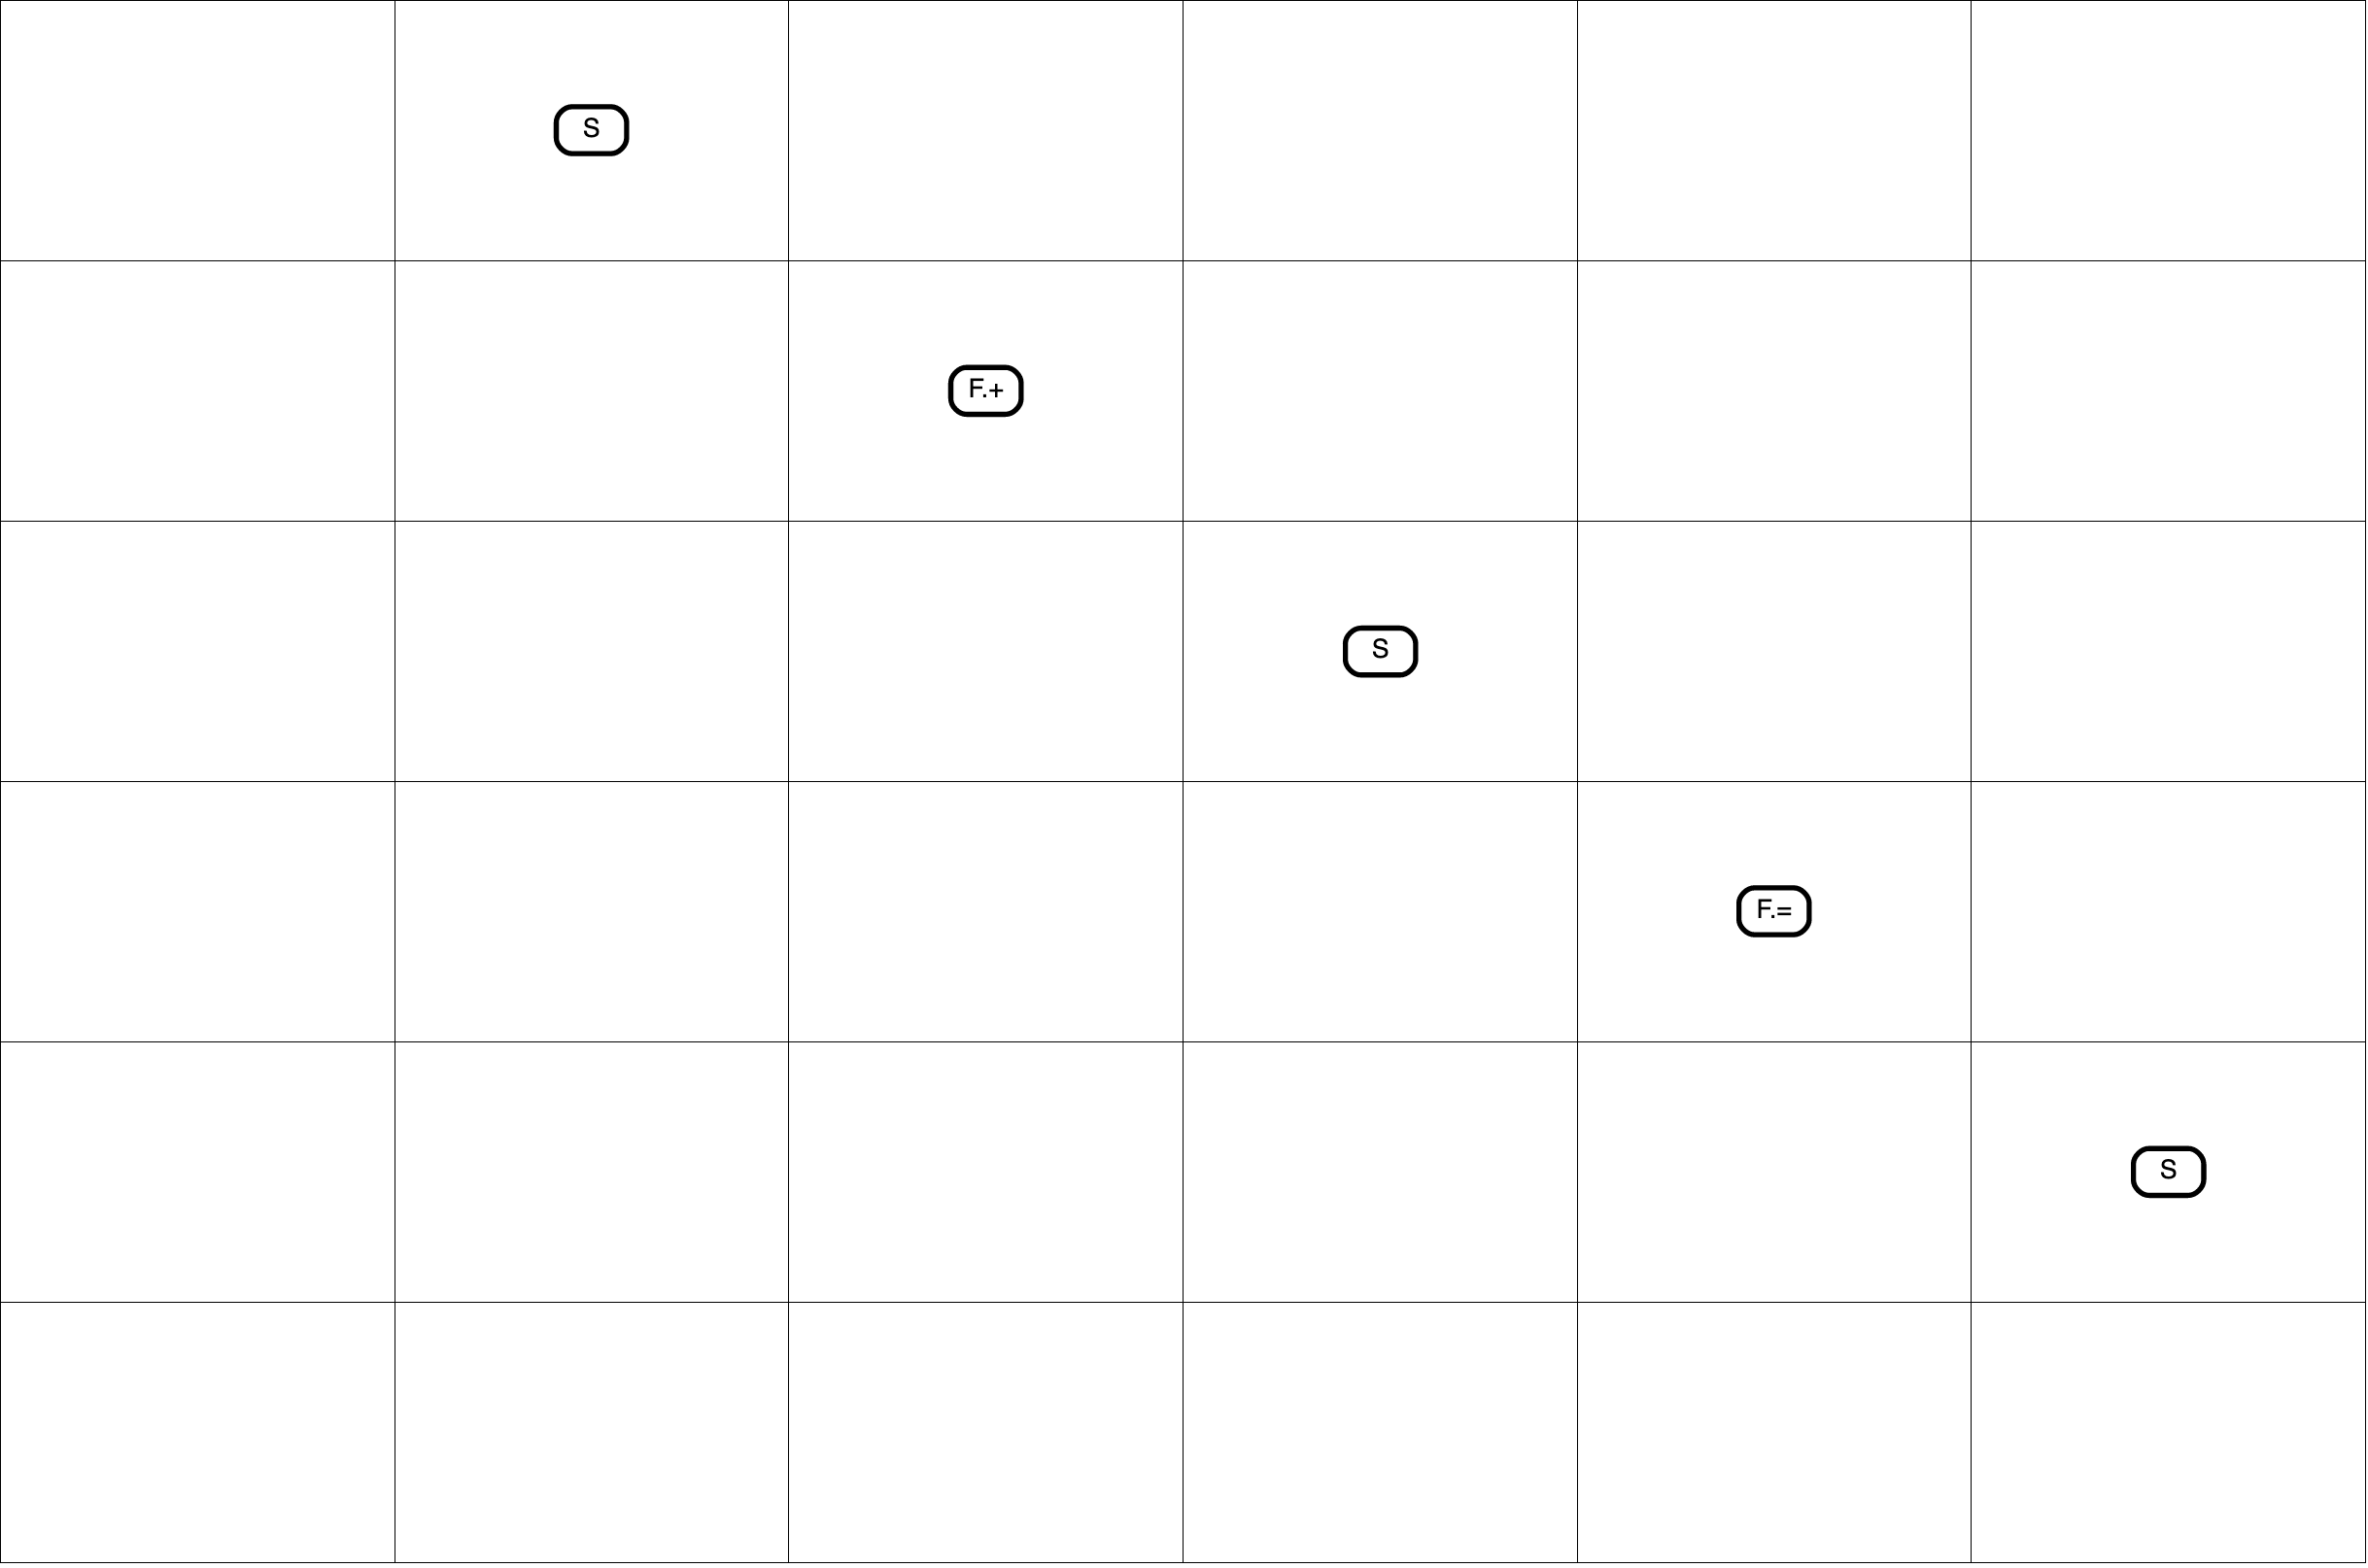
\includegraphics[width=2cm]{../figures/parse1.png}
%    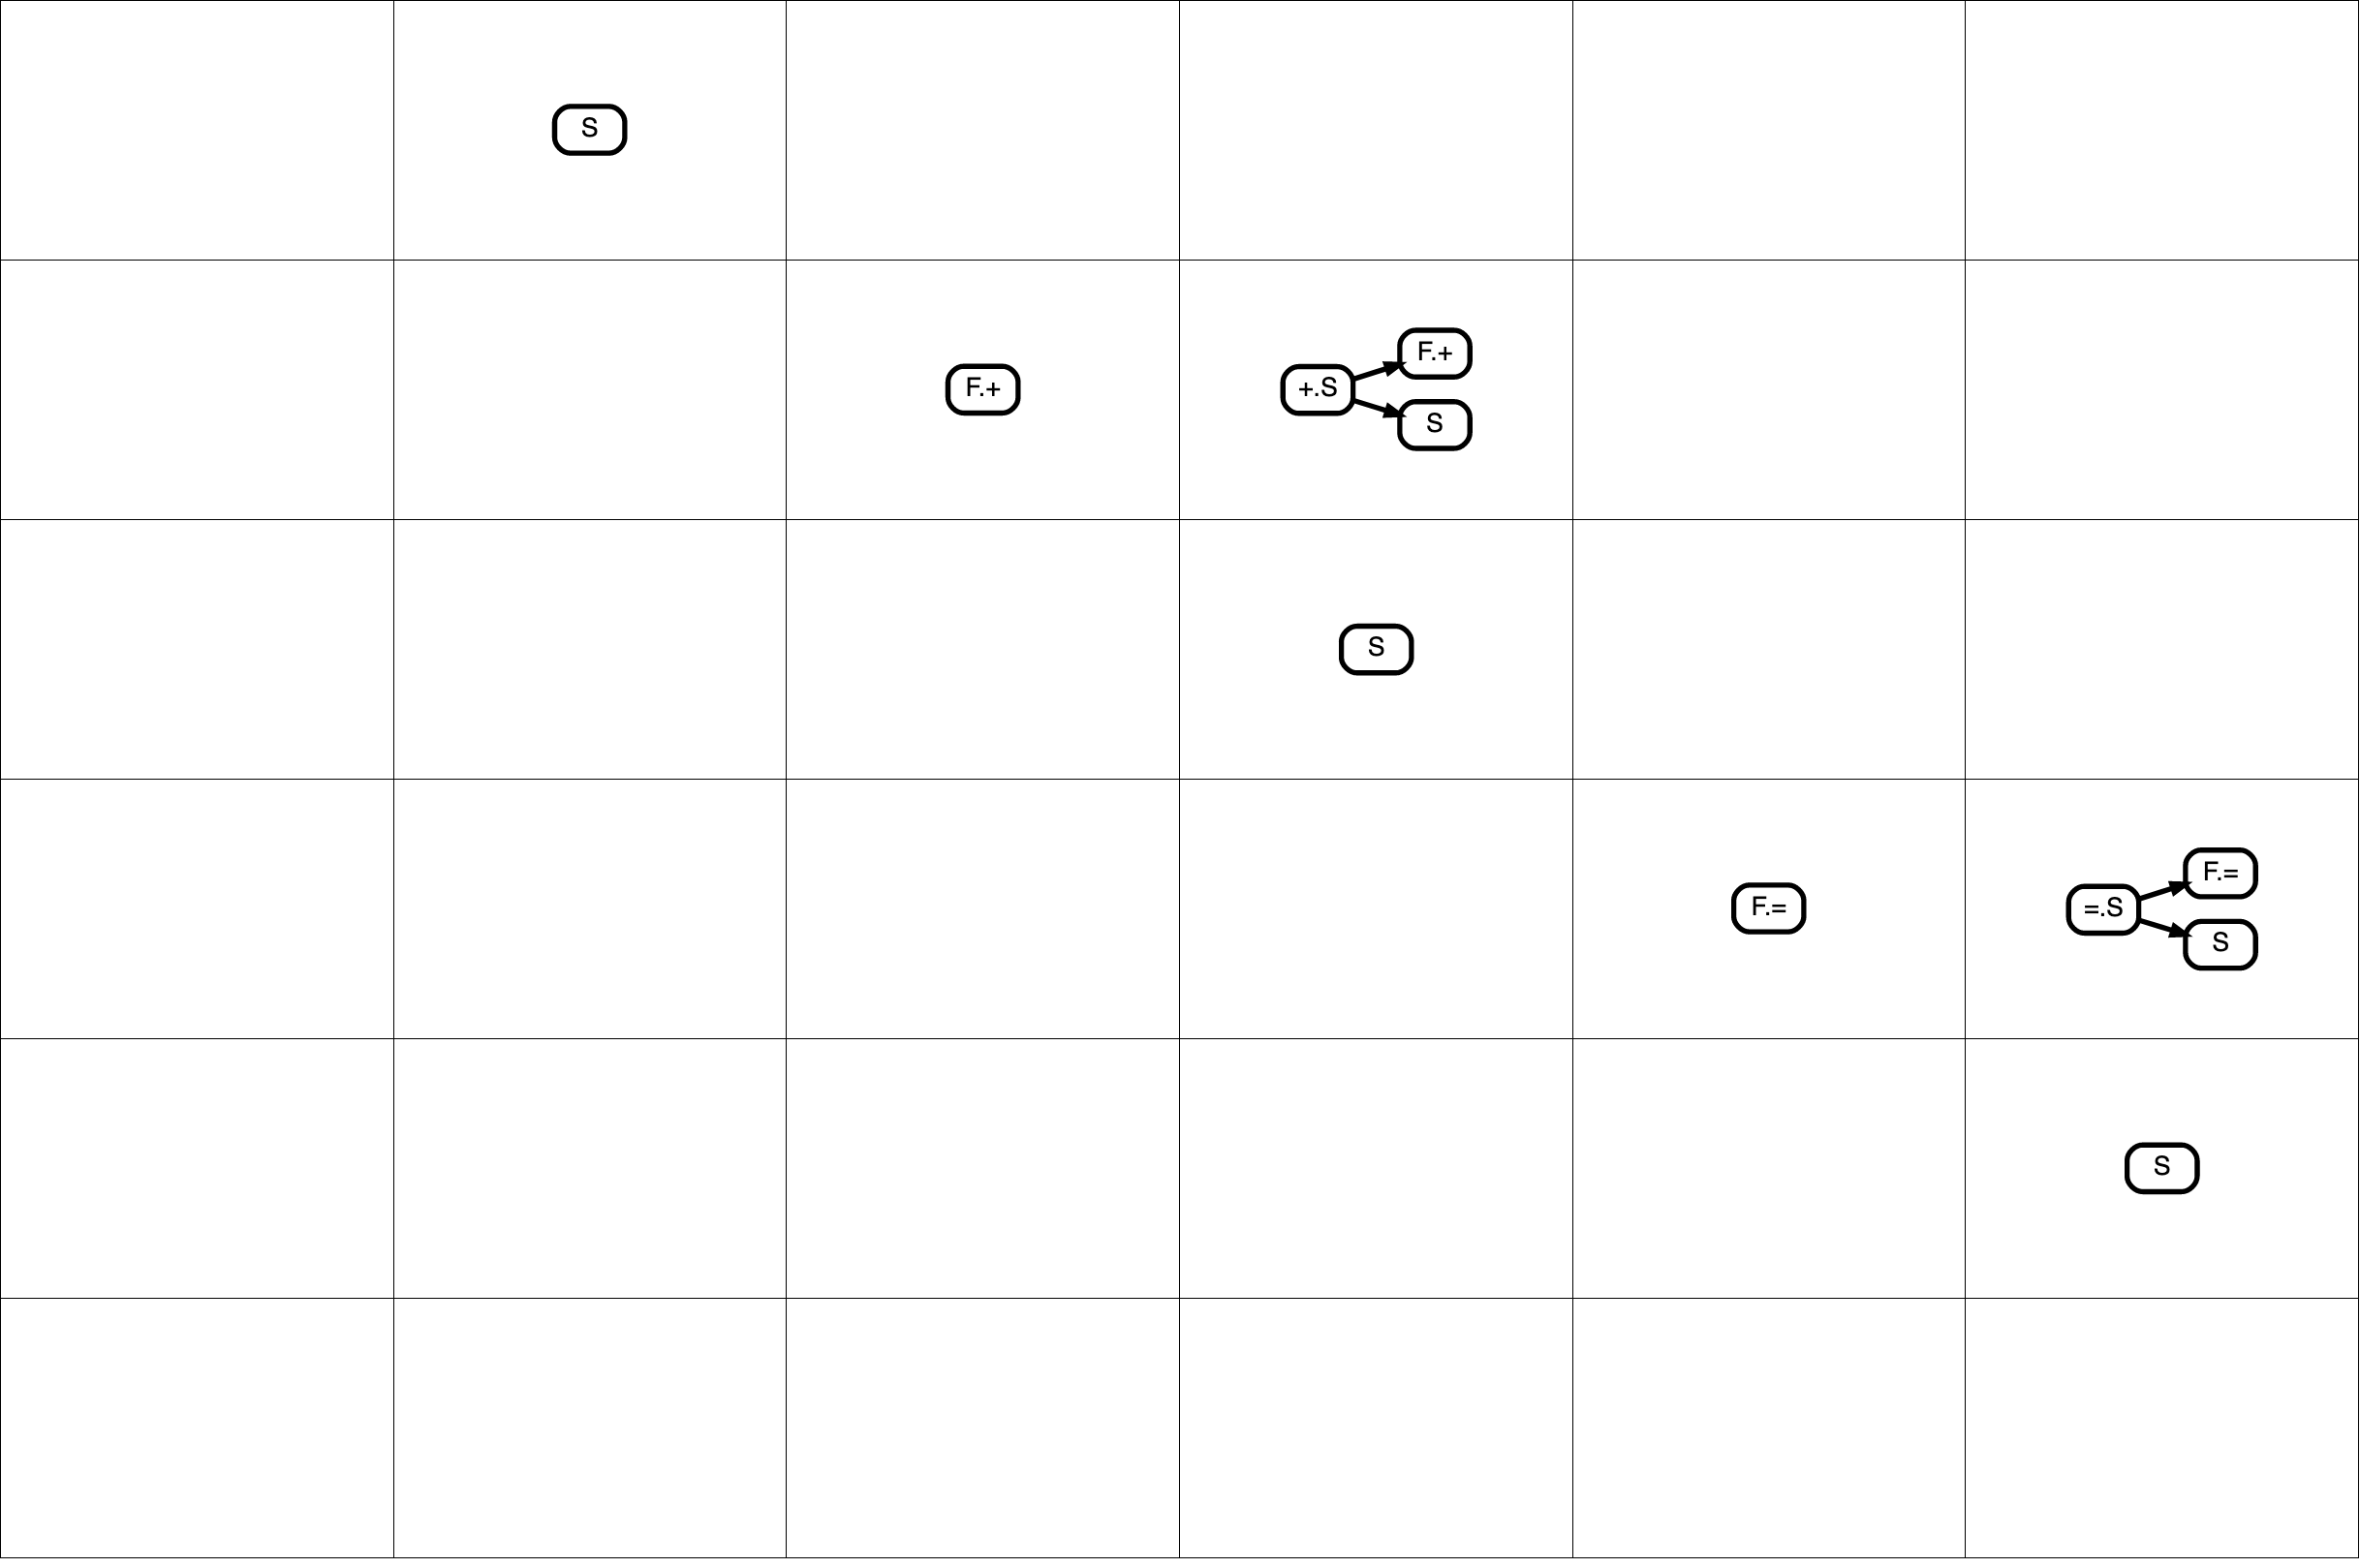
\includegraphics[width=2cm]{../figures/parse2.png}
%    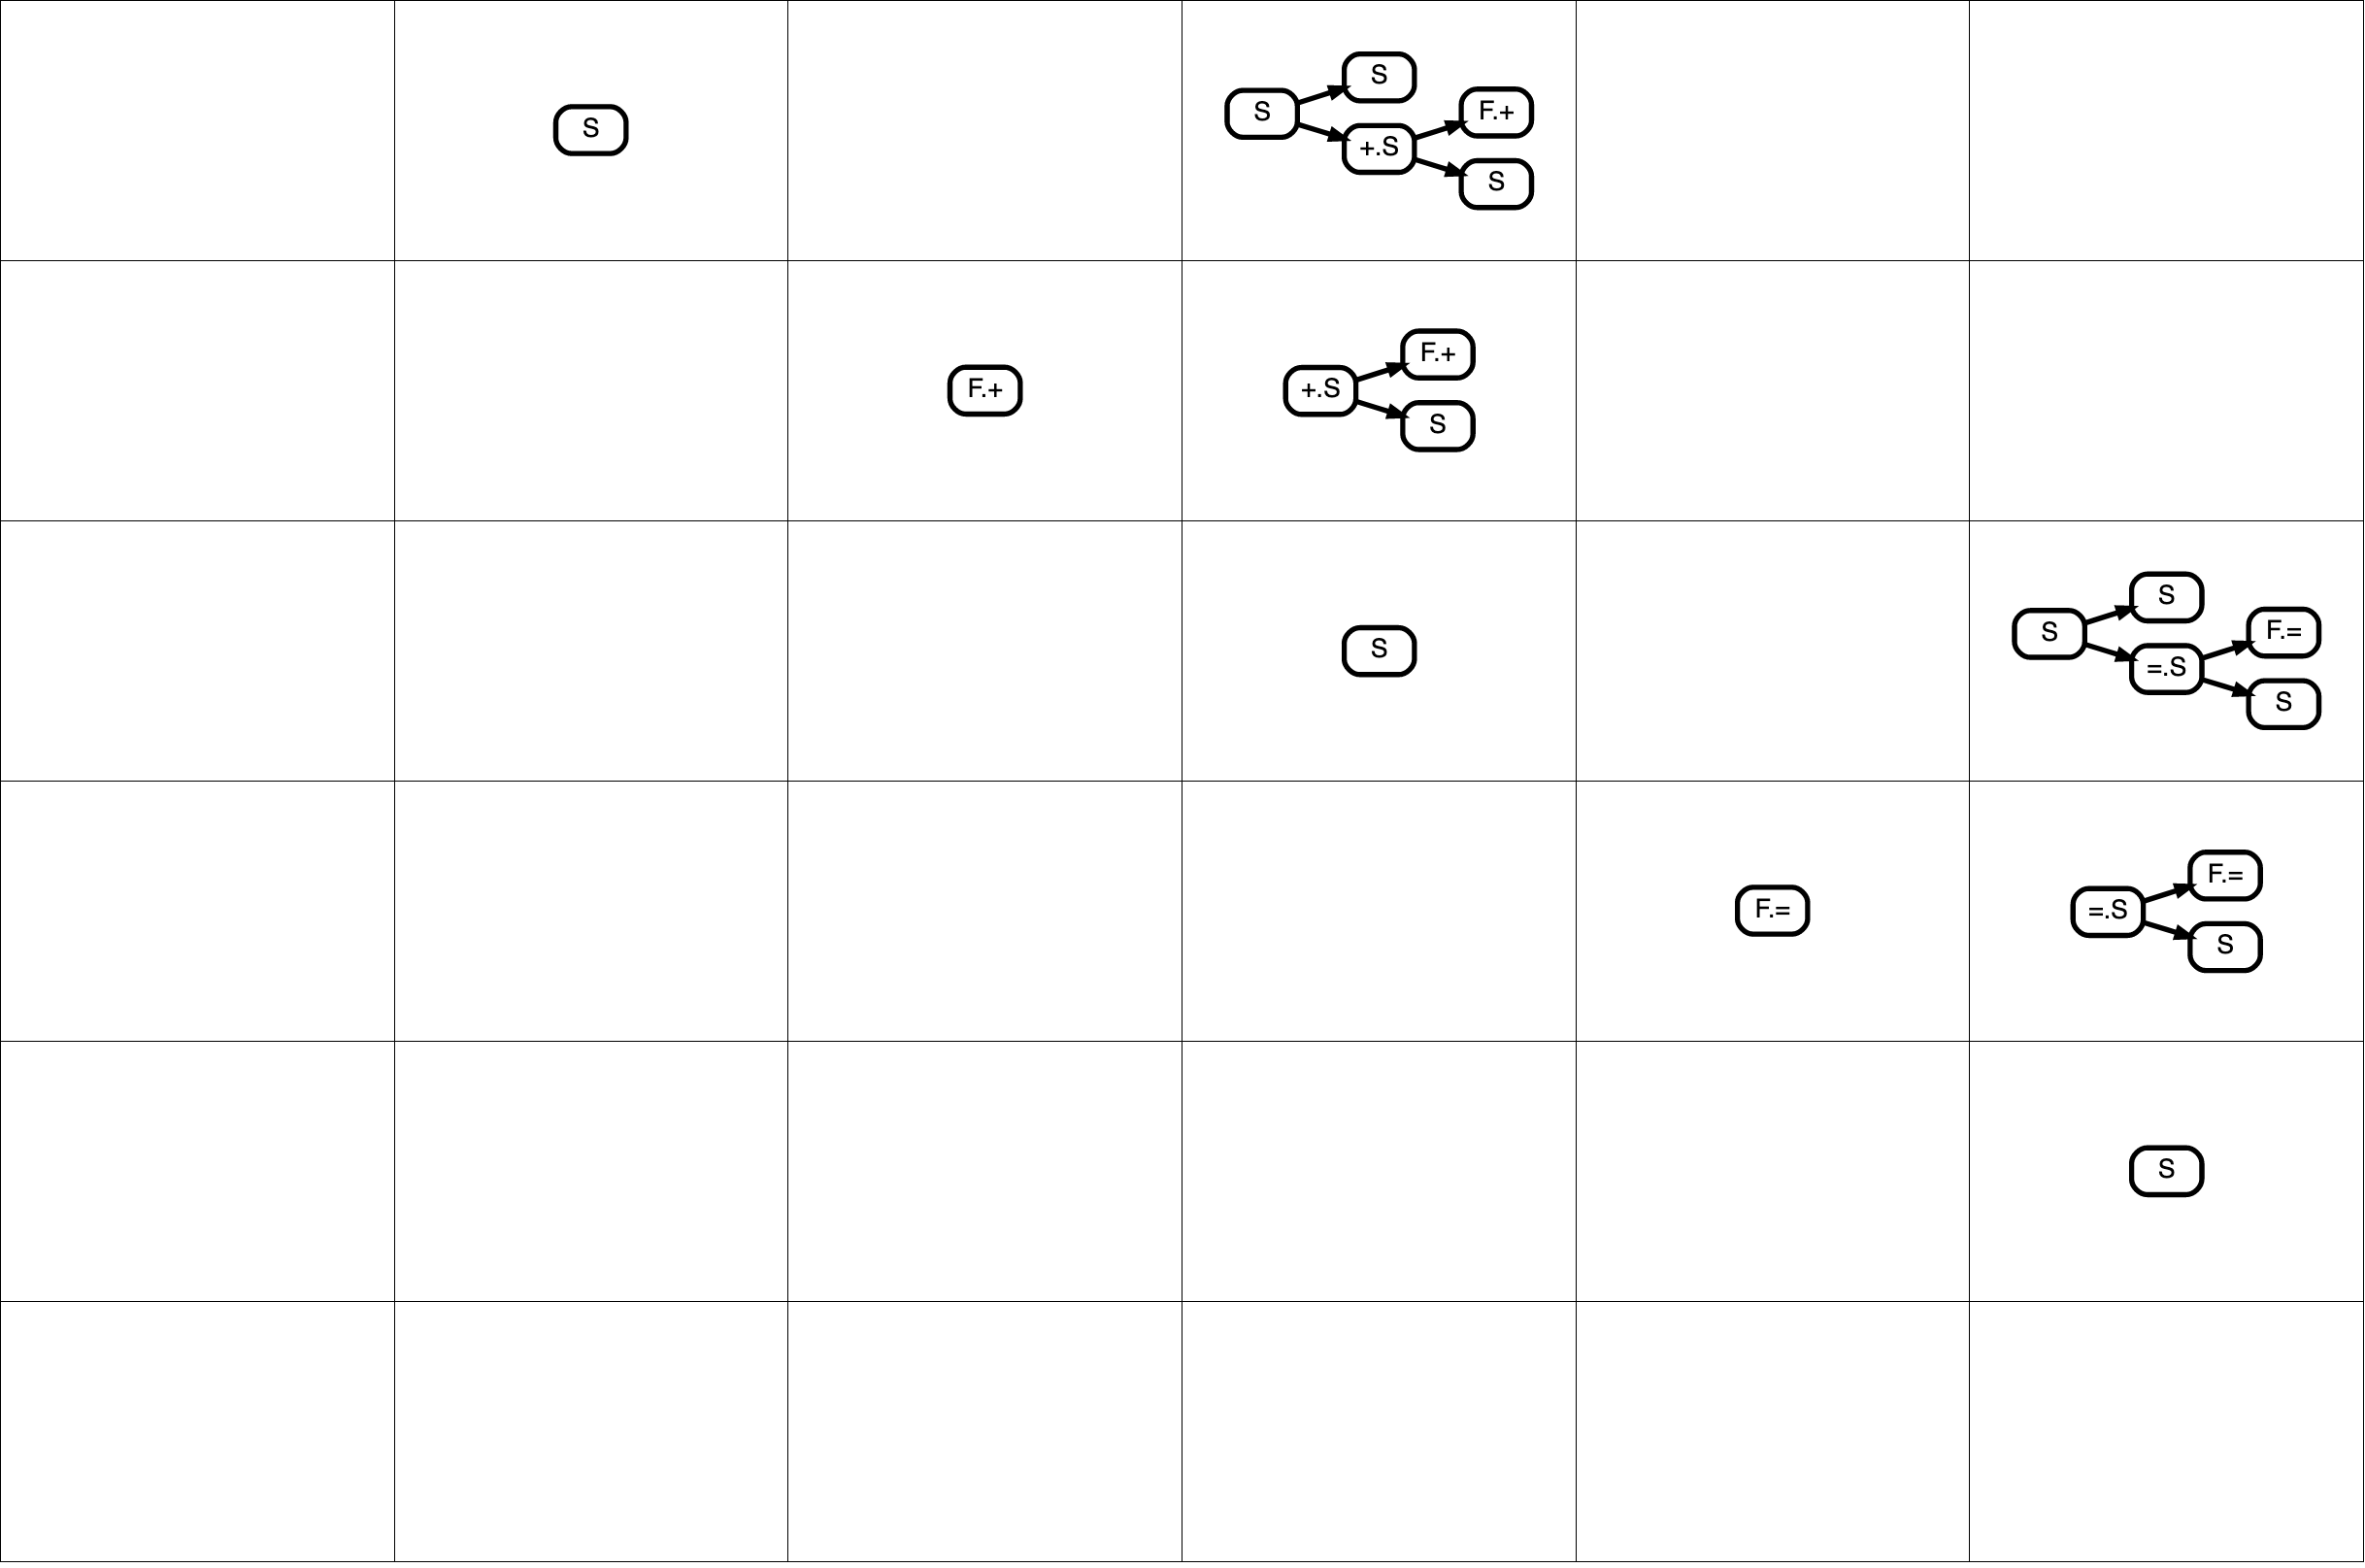
\includegraphics[width=2cm]{../figures/parse3.png}
%    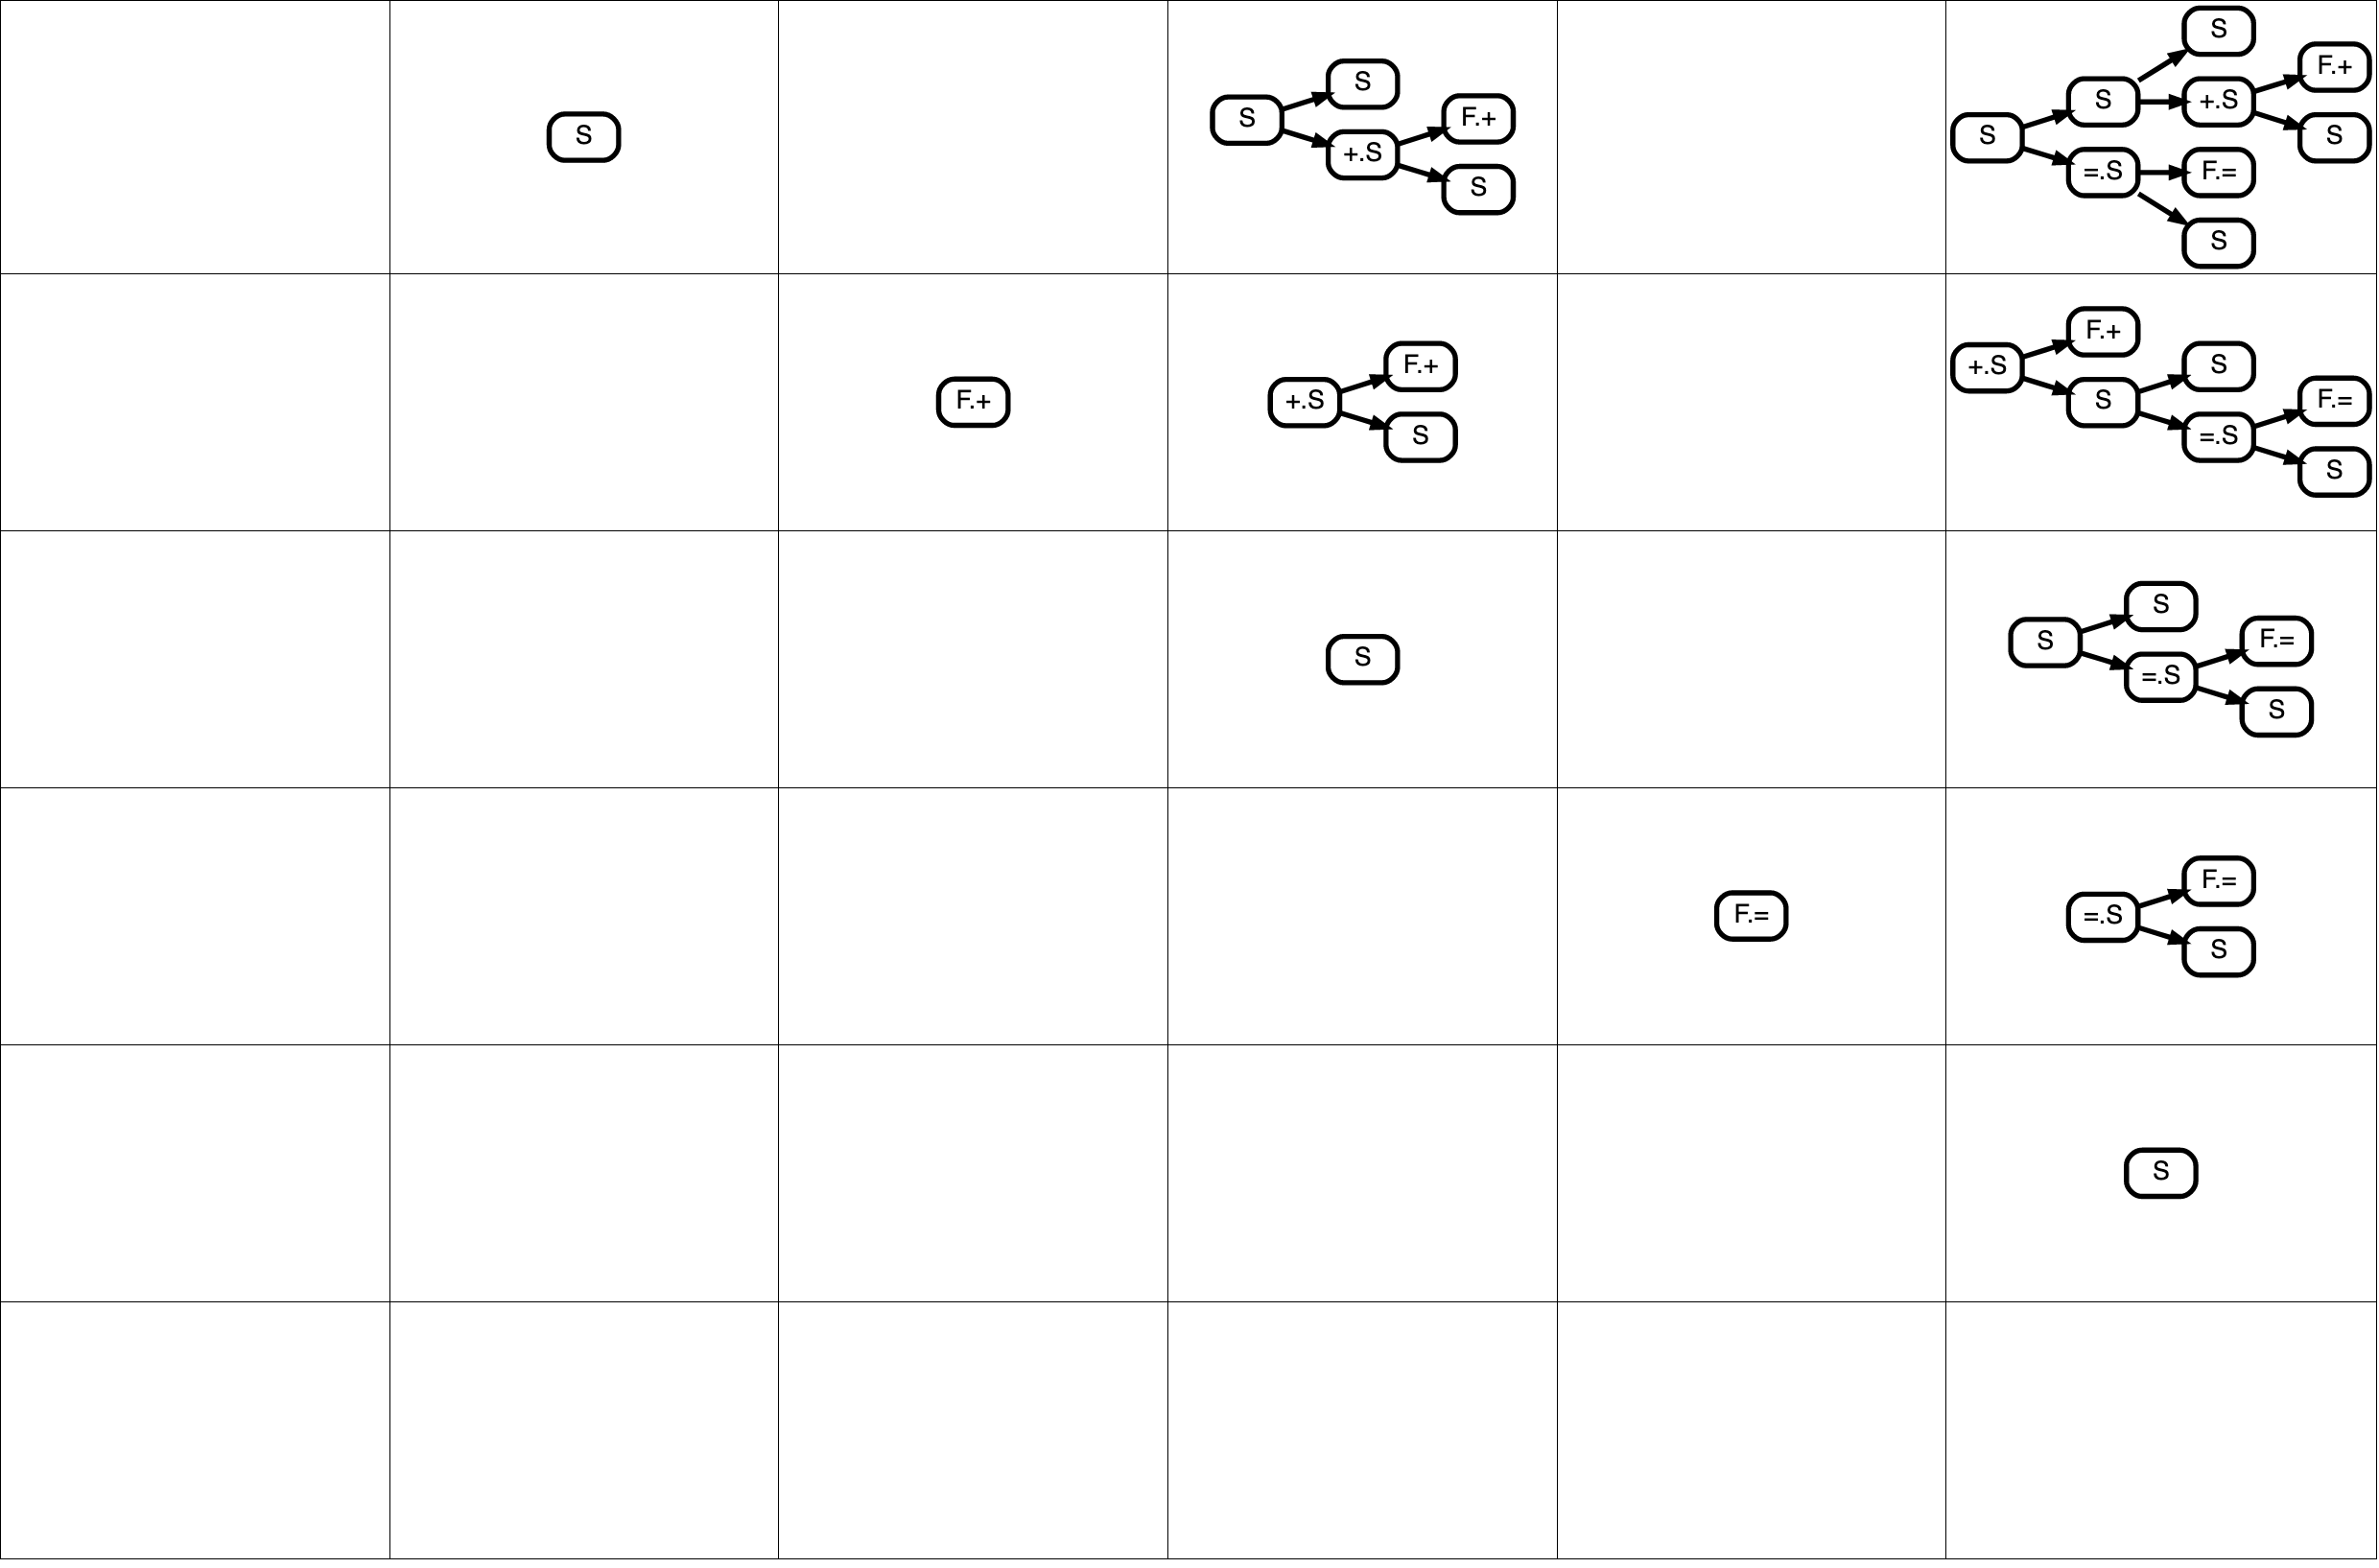
\includegraphics[width=2cm]{../figures/parse4.png}
%\end{figure}

\newcommand\ddd{\Ddots}
\newcommand\vdd{\Vdots}
\newcommand\cdd{\Cdots}
\newcommand\lds{\ldots}
\newcommand\vno{\varnothing}
\newcommand{\ts}[1]{\textsuperscript{#1}}
\newcommand\non{1\ts{st}}
\newcommand\ntw{2\ts{nd}}
\newcommand\nth{3\ts{rd}}
\newcommand\nfo{4\ts{th}}
\newcommand\nfi{5\ts{th}}
\newcommand\nsi{6\ts{th}}
\newcommand\nse{7\ts{th}}
\newcommand{\vs}[1]{\sigma_{#1}^{\shur}}
\newcommand{\gs}[1]{\gamma_{#1}^{\shur}}
\newcommand{\bs}[1]{\beta_{#1}^{\shur}}
\newcommand{\qs}[1]{\alpha_{#1}^{\shur}}
\newcommand\rcr{\rowcolor{black!15}}
\newcommand\rcw{\rowcolor{white}}
\newcommand\pcd{\cdot}
\newcommand\pcp{\phantom\cdot}
\newcommand\ppp{\phantom{\nse}}
\newcommand\hhg[1]{\tikz[overlay]\node[rectangle,fill=black!15,draw=none,text opacity =1] {$#1$};}

Our algorithm produces set of concrete syntax trees (CSTs) for a given valid string. Otherwise, if the string is invalid, the algorithm generates a set of admissible corrections, alongside their CSTs.

\section{Coarsening and simplification of subexpressions}

Depicted below is a SAT tensor representing \hlgray{$\sigma_1\:\sigma_2\:\sigma_3$}$\:\_\:\ldots\:\_$ where shaded regions demarcate known bitvector literals $\mathcal{L}_{r,c}$ (i.e., representing established nonterminal forests) and unshaded regions correspond to bitvector variables $\mathcal{V}_{r,c}$ (i.e., representing seeded nonterminal forests to be solved) for an incomplete string. Since $\mathcal{L}_{r,c}$ are fixed, we precompute them outside the SAT solver.

Clearly, solving complexity is highly dependent on the string length. For the sake of complexity, it would be convenient if well-formed subexpressions could be collapsed into a single nonterminal, or multiple nonterminals (in case of ambiguity). Naturally, this raises the question of when can partial derivations be simplified, i.e., under what circumstances is the following reduction admissible?

\begin{figure}[H]
\[
\mathbf{M}^* = \begin{pNiceArray}{ccccccc}[margin, extra-margin=2pt,colortbl-like, xdots/line-style=loosely dotted]
\vno & \rcr \vs{1} & \mathcal{L}_{1,3} & \mathcal{L}_{1,3} & \rcw \mathcal{V}_{1,4} & \cdd & \mathcal{V}_{1,n} \\
\vdd & \ddd        & \rcr\vs{2}        & \mathcal{L}_{2,3} & \rcw\vdd               &      & \vdd \\
     &             &                   & \rcr\vs{3}        & \rcw                   &      & \\
     &             &                   &                   & \mathcal{V}_{4,4}      &      & \\
     &             &                   &                   &                        & \ddd & \\
     &             &                   &                   &                        &      & \mathcal{V}_{n,n} \\
\vno & \cdd        &                   &                   &                        &      & \vno
\end{pNiceArray} \equiv
\begin{pNiceArray}{ccccc}[margin, extra-margin=2pt,colortbl-like, xdots/line-style=loosely dotted]
\vno & \rcr\mathcal{L}_{1,3} & \rcw\mathcal{V}_{1,4} & \cdd & \mathcal{V}_{1,n} \\
\vdd & \ddd                  & \mathcal{V}_{2,4}     &      & \vdd \\
     &                       &                       & \ddd & \\
     &                       &                       &      & \mathcal{V}_{n,n} \\
\vno & \cdd                  &                       &      & \vno
\end{pNiceArray}
\]
\end{figure}

This transformation is admissible when the subexpression is ``complete'', i.e., its derivation cannot be altered by appending or prepending text. For example, the string \texttt{( - b )} is morally \textit{complete} in the sense that inserting adjacent text should not alter the interior derivation, while \texttt{- b} is not, as introducing adjacent text (e.g., \texttt{a - b}) may alter the derivation of its contents depending on the structure of the CFG. This question can be reduced to a quotient: Does there exist another nonterminal, when so adjoined that will ``strip away'' any tokens, leading to another derivation?

More formally, given an arbitrary (potentially ambiguous) context free grammar $\mathcal{G}: \mathbb{G}$, and string $\alpha: \Sigma^\ast$, is there a decision procedure that returns whether appending and/or prepending symbols can alter the parse forest of $\alpha$? In other words, we want a function $F: (\mathbb{G} \times \Sigma^\ast) \rightarrow \mathbb{B}$ that returns whether $\alpha$'s parse forest according to $\mathcal{G}$ is unique over $\beta\alpha\gamma$, for all $\beta, \gamma: \Sigma^\ast$.

Specifically, let $\Lambda_\alpha$ denote the set of all parse trees that are generated by the string $\alpha$ using $\mathcal{G}$, and consider $\bm\Lambda_{\alpha}$, the union of all parse trees and their subtrees that (1) can be generated by $\beta\alpha\gamma$ using $\mathcal{G}$ for arbitrary $\beta, \gamma \in \Sigma^\ast$, and (2) have a leaf in $\alpha$. We call the parse forest $\Lambda_\alpha$ \textit{unique} iff $\forall t \in \bm\Lambda_{\alpha}\exists t' \in \Lambda_\alpha$, such that $t$ is either a subtree of $t'$, or $t'$ is a proper subtree of $t$.

\begin{equation*}
  M^*(\mathcal{G}, \beta\alpha\gamma)=
\begin{tikzpicture}[
  scale=0.4,
  baseline,
  label distance=10pt % added
]

\matrix [matrix of math nodes,left delimiter=(,right delimiter=),row sep=0.1cm,column sep=0.1cm] (m) {
\varnothing & \beta_1^\shri & \phantom{\cdots} & \,\Lambda_{\beta}\,  &        &                      & \phantom{\qs{|\alpha|}} &        &                      & \smash{\Lambda_{\beta\alpha\gamma}^*}      \\
            &               & \phantom{\ddots} & \phantom{\vdots}     &        & \bm\Lambda_\alpha^\shup &                  &        &                      &        \\
            &               &                  & \bs{|\beta|}         &        &                      &                  &        &                      & \phantom{\bs{|\beta|}}       \\
            &               &                  &                      & \qs{1} & \phantom{\cdots}     & \Lambda_{\alpha} &        &                      & \phantom{\vs{j}} \\
            &               &                  &                      &        & \phantom{\ddots}     & \phantom{\vdots} &        & \bm\Lambda_\alpha^\shri &        \\
            &               &                  &                      &        &                      & \qs{|\alpha|}           &        &                      & \phantom{\qs{|\alpha|}}      \\
            &               &                  &                      &        &                      &                  & \gs{1} & \phantom{\cdots}     & \Lambda_{\gamma}\vphantom{\gs{1}} \\
            &               &                  &                      &        &                      &                  &        & \phantom{\ddots}     & \phantom{\vdots} \\
            &               &                  &                      &        &                      &                  &        &                      & \gamma_{|\gamma|}^\shup      \\
\varnothing &               &                  &                      &        &                      &                  &        &                      & \varnothing\\
};

\draw[loosely dotted] (m-1-1.south) -- (m-10-1.north);
\draw[loosely dotted] (m-1-1.south east) -- (m-10-10.north west);
\draw[loosely dotted] (m-10-1.east) -- (m-10-10.west);

% β
\draw[loosely dotted] (m-1-2.south east) -- ([xshift=0.3cm]m-3-4.north west);
\draw[loosely dotted] (m-1-2.east) -- (m-1-4.west);
\draw[loosely dotted] (m-1-4.south) -- (m-3-4.north);

\draw[dashed] (m-1-4.north east) -- (m-3-4.south east);
\draw[dashed] (m-3-4.south east) -- (m-3-10.south east);
\draw[dashed] (m-1-7.north east) -- (m-6-7.south east);
\draw[dashed] (m-6-7.south east) -- (m-6-10.south east);

% α
\draw[loosely dotted] (m-4-5.south east) -- ([xshift=0.45cm,yshift=-0.2cm]m-6-7.north west);
\draw[loosely dotted] (m-4-5.east) -- (m-4-7.west);
\draw[loosely dotted] (m-4-7.south) -- (m-6-7.north);

% γ
\draw[loosely dotted] (m-7-8.south east) -- ([xshift=-0.1cm,yshift=-0.3cm]m-9-10.north west);
\draw[loosely dotted] (m-7-8.east) -- (m-7-10.west);
\draw[loosely dotted] (m-7-10.south) -- (m-9-10.north);
\node[
    fit=(m-1-2)(m-1-4),
    inner xsep=0,inner ysep=10pt,
    above delimiter=\{,
    label=above:$\beta$
] {};

\node[
    fit=(m-7-10)(m-9-10),
    inner xsep=14pt,inner ysep=0,
    right delimiter=\},
    label=right:$\gamma$
] {};

\end{tikzpicture}
\end{equation*}

Let $\bm\Lambda_{\alpha}^{\shur}$ be defined as $\bm\Lambda_{\alpha}^{\shur}:=\bm\Lambda_{\alpha}^\shup\cup\bm\Lambda_{\alpha}^\shri$, the union of all right- and left-quotients of $\alpha$.

Claim #1: The parse forest for $\alpha$ is unique when $\bm\Lambda_{\alpha}^{\shur} = \varnothing$.

Question: Claim #1 is sufficient, but is it necessary?

\pagebreak\section{Backpropagation of error}

%    Although holes may occur anywhere, let us consider two cases in which $\Sigma^+$ is strictly left- or right-constrained, i.e., $\highlight{x}z, x\highlight{z}: \Sigma^{|x|+|z|}$.

Valiant's $\otimes$-operator, which yields the set of productions unifying known factors in a binary CFG, naturally implies the existence of a left- and right-quotient, which yield the set of nonterminals that may appear the right or left side of a known factor and its corresponding root. In other words, a known factor not only implicates subsequent expressions that can be derived from it, but also adjacent factors that may be composed with it to form a given derivation.

\begin{table}[H]
\resizebox{\textwidth}{!}{
  \begin{tabular}{ccccc}
    Valiant's $\otimes$-operator && Left Quotient && Right Quotient \\\\
    $x \otimes z := \big\{\;w \mid (w \rightarrow x z)\in P\;\big\}$ &&
    $\frac{\partial w}{\partial \cev{x}} := \big\{\;z \mid (w \rightarrow x z)\in P\;\big\}$ &&
    $\frac{\partial w}{\partial \vec{z}} := \big\{\;x \mid (w \rightarrow x z)\in P\;\big\}$ \\\\
    \begin{tabular}{|c|c|}
      \hline
      \cellcolor{black!15}\hspace{-0.5mm}$x$\hspace{-0.5mm} & \hspace{-0.95mm}$w$\hspace{-0.95mm} \\ \hline
      \multicolumn{1}{c|}{~} & \cellcolor{black!15}\hspace{-0.95mm}$z$\hspace{-0.95mm} \\
      \cline{2-2}
    \end{tabular} &&
    \begin{tabular}{|c|c|}
      \hline
      \cellcolor{black!15}\hspace{-0.5mm}$x$\hspace{-0.5mm} & \cellcolor{black!15}\hspace{-0.95mm}$w$\hspace{-0.95mm} \\ \hline
      \multicolumn{1}{c|}{~} & \hspace{-0.95mm}$z$\hspace{-0.95mm} \\
      \cline{2-2}
    \end{tabular} &&
    \begin{tabular}{|c|c|}
      \hline
      \hspace{-0.5mm}$x$\hspace{-0.5mm} & \cellcolor{black!15}\hspace{-0.95mm}$w$\hspace{-0.95mm} \\ \hline
      \multicolumn{1}{c|}{~} & \cellcolor{black!15}\hspace{-0.95mm}$z$\hspace{-0.95mm} \\
      \cline{2-2}
    \end{tabular}
  \end{tabular}
}
\end{table}

\noindent The left quotient coincides with the derivative operator first proposed by Brzozowski~\cite{brzozowski1964derivatives} and Antimirov~\cite{antimirov1996partial} over regular languages, lifted into the context-free setting (our work). When the root and LHS are fixed, e.g., $\frac{\partial S}{\partial \cev{x}}: (\cev{V} \rightarrow S) \rightarrow \vec{\mathcal{V}}$ returns the set of admissible nonterminals to the RHS. One may also consider a gradient operator, $\cev{\nabla} S: (\cev{\mathcal{V}} \rightarrow S) \rightarrow \vec{\mathcal{V}}$, which simultaneously tracks the partials with respect to a set of multiple LHS nonterminals produced by a fixed root.

%  These operators in the context-free setting respect linearity. The $\oplus$ case is trivial. For $\otimes$, let us consider the left quotient. Its symmetric case is left as an exercise for the reader:
%
%  $\frac{\partial}{\partial x}(f\otimes g) = \frac{\partial f}{\partial x}\otimes g \oplus f\otimes\frac{\partial g}{\partial x}$
%
%  TODO: prove the product rule holds for CFG reachability.

If the root itself is unknown, we can define an operator, $\mathcal{H}_{\mathcal{W}\subseteq\mathcal{V}}: (\cev{\mathcal{V}}\times\vec{\mathcal{V}}\times\mathcal{W}) \rightarrow (\vec{\mathcal{V}}\times\vec{\mathcal{V}}\rightarrow\mathcal{W})$, which tracks second-order partial derivatives for all roots in $\mathcal{W}$. Unlike differential calculus on smooth manifolds, partials in this calculus do not necessarily commute depending on the CFG.

\definecolor{R}{RGB}{202,65,55}
\definecolor{G}{RGB}{151,216,56}
\definecolor{W}{RGB}{255,255,255}
\definecolor{X}{RGB}{65,65,65}

\newcommand{\TikZRubikFaceLeft}[9]{\def\myarrayL{#1,#2,#3,#4,#5,#6,#7,#8,#9}}
\newcommand{\TikZRubikFaceRight}[9]{\def\myarrayR{#1,#2,#3,#4,#5,#6,#7,#8,#9}}
\newcommand{\TikZRubikFaceTop}[9]{\def\myarrayT{#1,#2,#3,#4,#5,#6,#7,#8,#9}}
\newcommand{\BuildArray}{\foreach \X [count=\Y] in \myarrayL%
{\ifnum\Y=1%
\xdef\myarray{"\X"}%
\else%
\xdef\myarray{\myarray,"\X"}%
\fi}%
\foreach \X in \myarrayR%
{\xdef\myarray{\myarray,"\X"}}%
\foreach \X in \myarrayT%
{\xdef\myarray{\myarray,"\X"}}%
\xdef\myarray{{\myarray}}%
}
\TikZRubikFaceLeft
{LA}{W}{W}
{W}{LB}{LC}
{LD}{W}{W}
\TikZRubikFaceRight
{W}{LK}{W}
{LC}{W}{LG}
{W}{LH}{W}
\TikZRubikFaceTop
{LA}{W}{LI}
{W}{W}{LJ}
{W}{LK}{W}
\BuildArray
\pgfmathsetmacro\radius{0.1}
\tdplotsetmaincoords{55}{135}

\showcellnumberfalse

\begin{figure}
  \[
  \begin{align*}
    o &\rightarrow \hiliD{so} \mid \hiliC{rs} \mid \hiliB{rr}\hspace{0.5pt} \mid \hiliA{oo}\\
    r &\rightarrow \hiliE{so} \mid \hiliH{ss}\hspace{0.4pt}\mid \hiliF{rr}\hspace{0.5pt} \mid \hiliK{os}\\
    s &\rightarrow \hiliL{so} \mid \hiliG{rs} \mid \hiliJ{or} \mid \hiliI{oo}
  \end{align*} \phantom{=} \mathcal{H}_{\{o\}} = \begin{pmatrix}
        \hiliA{\pder{^2 o}{\cev{o}\partial\vec{o}}} & \pder{^2 o}{\cev{o}\partial\vec{r}} & \pder{^2 o}{\cev{o}\partial\vec{s}}\\
        \pder{^2 o}{\cev{r}\partial\vec{o}} & \hiliB{\pder{^2 o}{\cev{r}\partial\vec{r}}} & \hiliC{\pder{^2 o}{\cev{r}\partial\vec{s}}}\\
        \hiliD{\pder{^2 o}{\cev{s}\partial\vec{o}}} & \pder{^2 o}{\cev{s}\partial\vec{r}} & \pder{^2 o}{\cev{s}\partial\vec{s}}
      \end{pmatrix}
%    \mathcal{J} = \begin{pmatrix}
%       \pder{o}{o} & \pder{o}{r} & \pder{o}{s}\\
%       \pder{r}{o} & \pder{r}{r} & \pder{r}{s}\\
%       \pder{s}{o} & \pder{s}{r} & \pder{s}{s}
%    \end{pmatrix}
  \]
  \hspace{-0.5cm}\begin{minipage}[l]{4.3cm}
  \scalebox{0.8}{\begin{tikzpicture}
    \clip (-3,-2.5) rectangle (3,2.5);
    \begin{scope}[tdplot_main_coords]
      \filldraw [canvas is yz plane at x=1.5] (-1.5,-1.5) rectangle (1.5,1.5);
      \filldraw [canvas is xz plane at y=1.5] (-1.5,-1.5) rectangle (1.5,1.5);
      \filldraw [canvas is yx plane at z=1.5] (-1.5,-1.5) rectangle (1.5,1.5);
      \foreach \X [count=\XX starting from 0] in {-1.5,-0.5,0.5}{
        \foreach \Y [count=\YY starting from 0] in {-1.5,-0.5,0.5}{
          \pgfmathtruncatemacro{\Z}{\XX+3*(2-\YY)}
          \pgfmathsetmacro{\mycolor}{\myarray[\Z]}
          \draw [thick,canvas is yz plane at x=1.5,shift={(\X,\Y)},fill=\mycolor] (0.5,0) -- ({1-\radius},0) arc (-90:0:\radius) -- (1,{1-\radius}) arc (0:90:\radius) -- (\radius,1) arc (90:180:\radius) -- (0,\radius) arc (180:270:\radius) -- cycle;
          \ifshowcellnumber
          \node[canvas is yz plane at x=1.5,shift={(\X+0.5,\Y+0.5)}] {\Z};
          \fi
          \pgfmathtruncatemacro{\Z}{2-\XX+3*(2-\YY)+9}
          \pgfmathsetmacro{\mycolor}{\myarray[\Z]}
          \draw [thick,canvas is xz plane at y=1.5,shift={(\X,\Y)},fill=\mycolor] (0.5,0) -- ({1-\radius},0) arc (-90:0:\radius) -- (1,{1-\radius}) arc (0:90:\radius) -- (\radius,1) arc (90:180:\radius) -- (0,\radius) arc (180:270:\radius) -- cycle;
          \ifshowcellnumber
          \node[canvas is xz plane at y=1.5,shift={(\X+0.5,\Y+0.5)},xscale=-1] {\Z};
          \fi
          \pgfmathtruncatemacro{\Z}{2-\YY+3*\XX+18}
          \pgfmathsetmacro{\mycolor}{\myarray[\Z]}
          \draw [thick,canvas is yx plane at z=1.5,shift={(\X,\Y)},fill=\mycolor] (0.5,0) -- ({1-\radius},0) arc (-90:0:\radius) -- (1,{1-\radius}) arc (0:90:\radius) -- (\radius,1) arc (90:180:\radius) -- (0,\radius) arc (180:270:\radius) -- cycle;
          \ifshowcellnumber
          \node[canvas is yx plane at z=1.5,shift={(\X+0.5,\Y+0.5)},xscale=-1,rotate=-90] {\Z};
          \fi
        }
      }
      \draw [decorate,decoration={calligraphic brace,amplitude=10pt,mirror},yshift=0pt, line width=1.25pt]
      (3,0) -- (3,3) node [black,midway,xshift=-8pt, yshift=-14pt] {\footnotesize $V_x$};
      \draw [decorate,decoration={calligraphic brace,amplitude=10pt},yshift=0pt, line width=1.25pt]
      (3,0) -- (0,-3) node [black,midway,xshift=-16pt, yshift=0pt] {\footnotesize $V_z$};
      \draw [decorate,decoration={calligraphic brace,amplitude=10pt},yshift=0pt, line width=1.25pt]
      (0,-3) -- (-3,-3) node [black,midway,xshift=-8pt, yshift=14pt] {\footnotesize $V_w$};
    \end{scope}
  \end{tikzpicture}}
  \end{minipage}
  \begin{minipage}[c]{3.5cm}
    \begin{align*}
      \mathcal{H}_{\{r\}} = & \begin{pmatrix}
         \pder{^2 r}{\cev{o}\partial\vec{o}} & \pder{^2 r}{\cev{o}\partial\vec{r}} & \hiliK{\pder{^2 r}{\cev{o}\partial\vec{s}}}\\
         \pder{^2 r}{\cev{r}\partial\vec{o}} & \hiliF{\pder{^2 r}{\cev{r}\partial\vec{r}}} & \pder{^2 r}{\cev{r}\partial\vec{s}}\\
         \hiliE{\pder{^2 r}{\cev{s}\partial\vec{o}}} & \pder{^2 r}{\cev{s}\partial\vec{r}} & \hiliH{\pder{^2 r}{\cev{s}\partial\vec{s}}}
      \end{pmatrix}
    \end{align*}
      \begin{align*}
      \mathcal{H}_{\{s\}} = & \begin{pmatrix}
         \hiliI{\pder{^2 s}{\cev{o}\partial\vec{o}}} & \hiliJ{\pder{^2 s}{\cev{o}\partial\vec{r}}} & \pder{^2 s}{\cev{o}\partial\vec{s}}\\
         \pder{^2 s}{\cev{r}\partial\vec{o}} & \pder{^2 s}{\cev{r}\partial\vec{r}} & \hiliG{\pder{^2 s}{\cev{r}\partial\vec{s}}}\\
         \hiliL{\pder{^2 s}{\cev{s}\partial\vec{o}}} & \pder{^2 s}{\cev{s}\partial\vec{r}} & \pder{^2 s}{\cev{s}\partial\vec{s}}
      \end{pmatrix}
    \end{align*}
  \end{minipage}
  \caption{CFGs are witnessed by a rank-3 tensor, whose inhabitants indicate CNF productions. Gradients in this setting effectively condition the parse tensor M by constraining the superposition of admissible parse forests.\vspace{-10pt}}
\end{figure}

\noindent By allowing the matrix $\mathcal{M}^*$ to contain bitvector variables representing holes in $\sigma$, we obtain a set of multilinear equations whose solutions exactly correspond to the set of admissible repairs and their corresponding parse forests. Specifically, the repairs coincide with holes in the superdiagonal $\mathcal{M}^*_{r+1 = c}$, and the parse forests occur along upper-triangular entries $\mathcal{M}^*_{r + 1 < c}$.
%
%%We precompute the shadow of fully-resolved substrings before feeding it to the SAT solver. If the substring is known, we can simply compute this directly outside the SAT solver. Shaded regions are bitvector literals and light regions correspond to bitvector variables.
%
%%We illustrate this fact in \S\ref{sec:error}:
%%
%%\begin{figure}[H]
%%    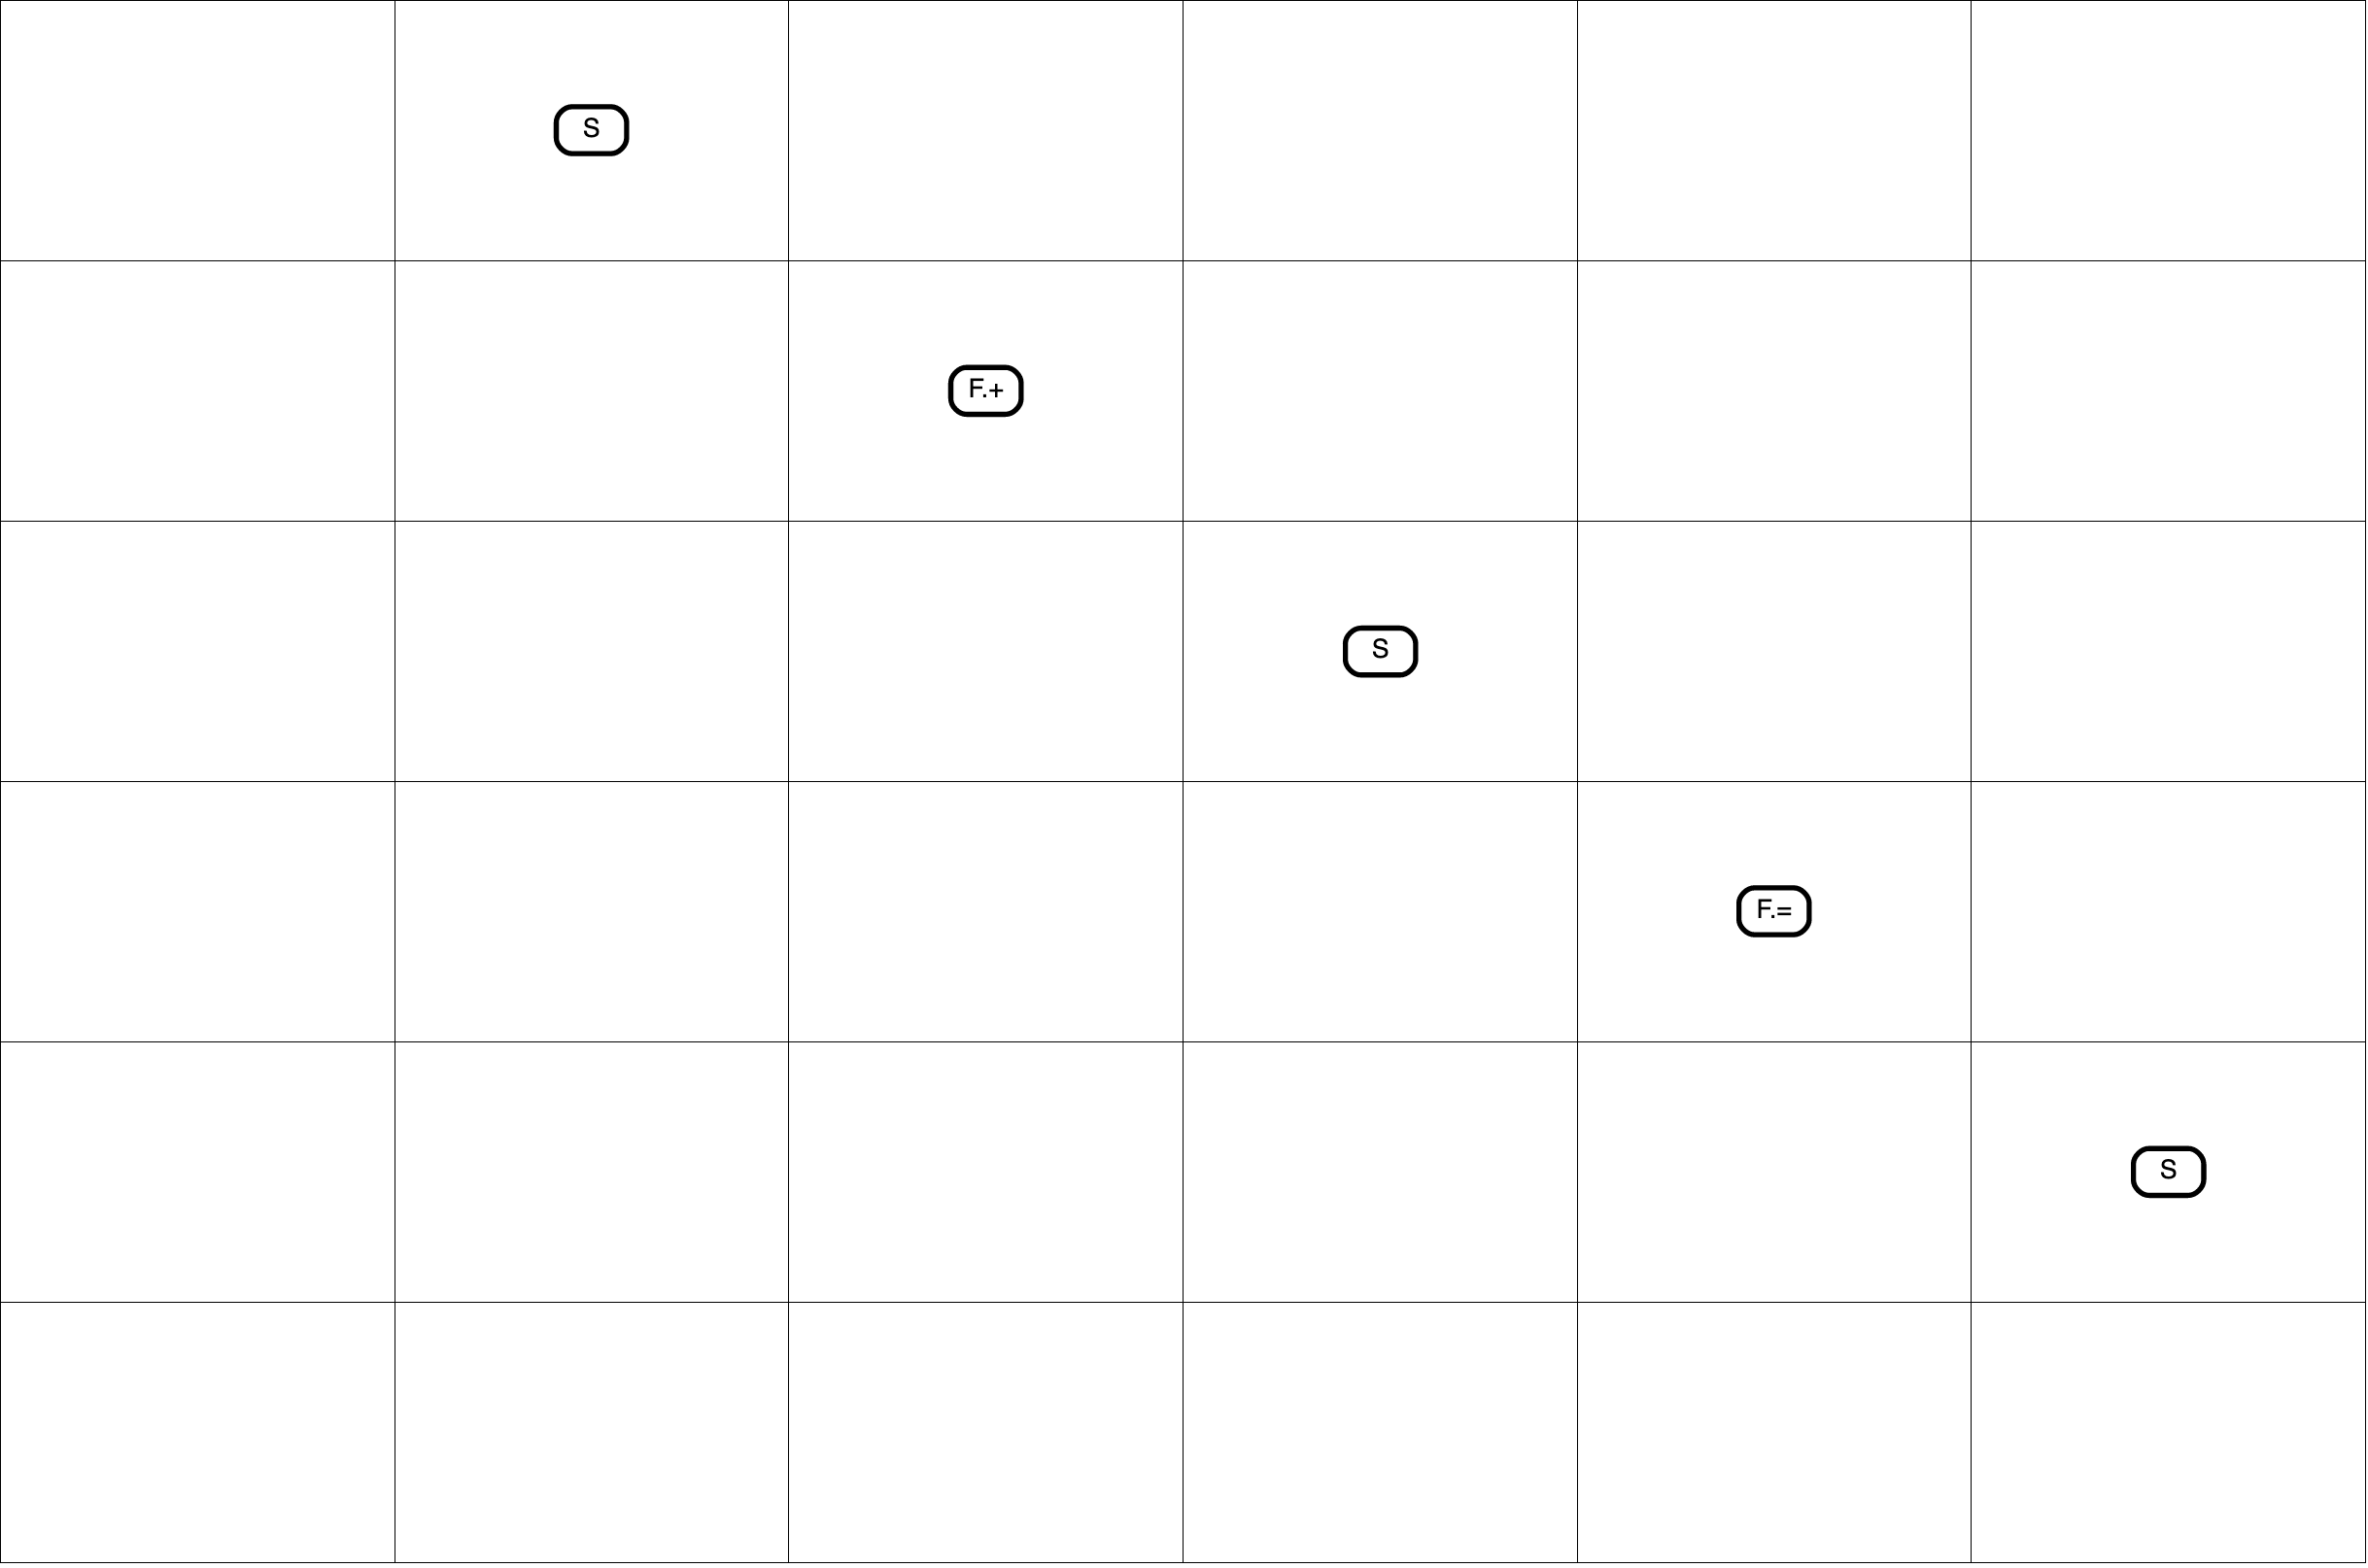
\includegraphics[width=2cm]{../figures/parse1.png}
%%    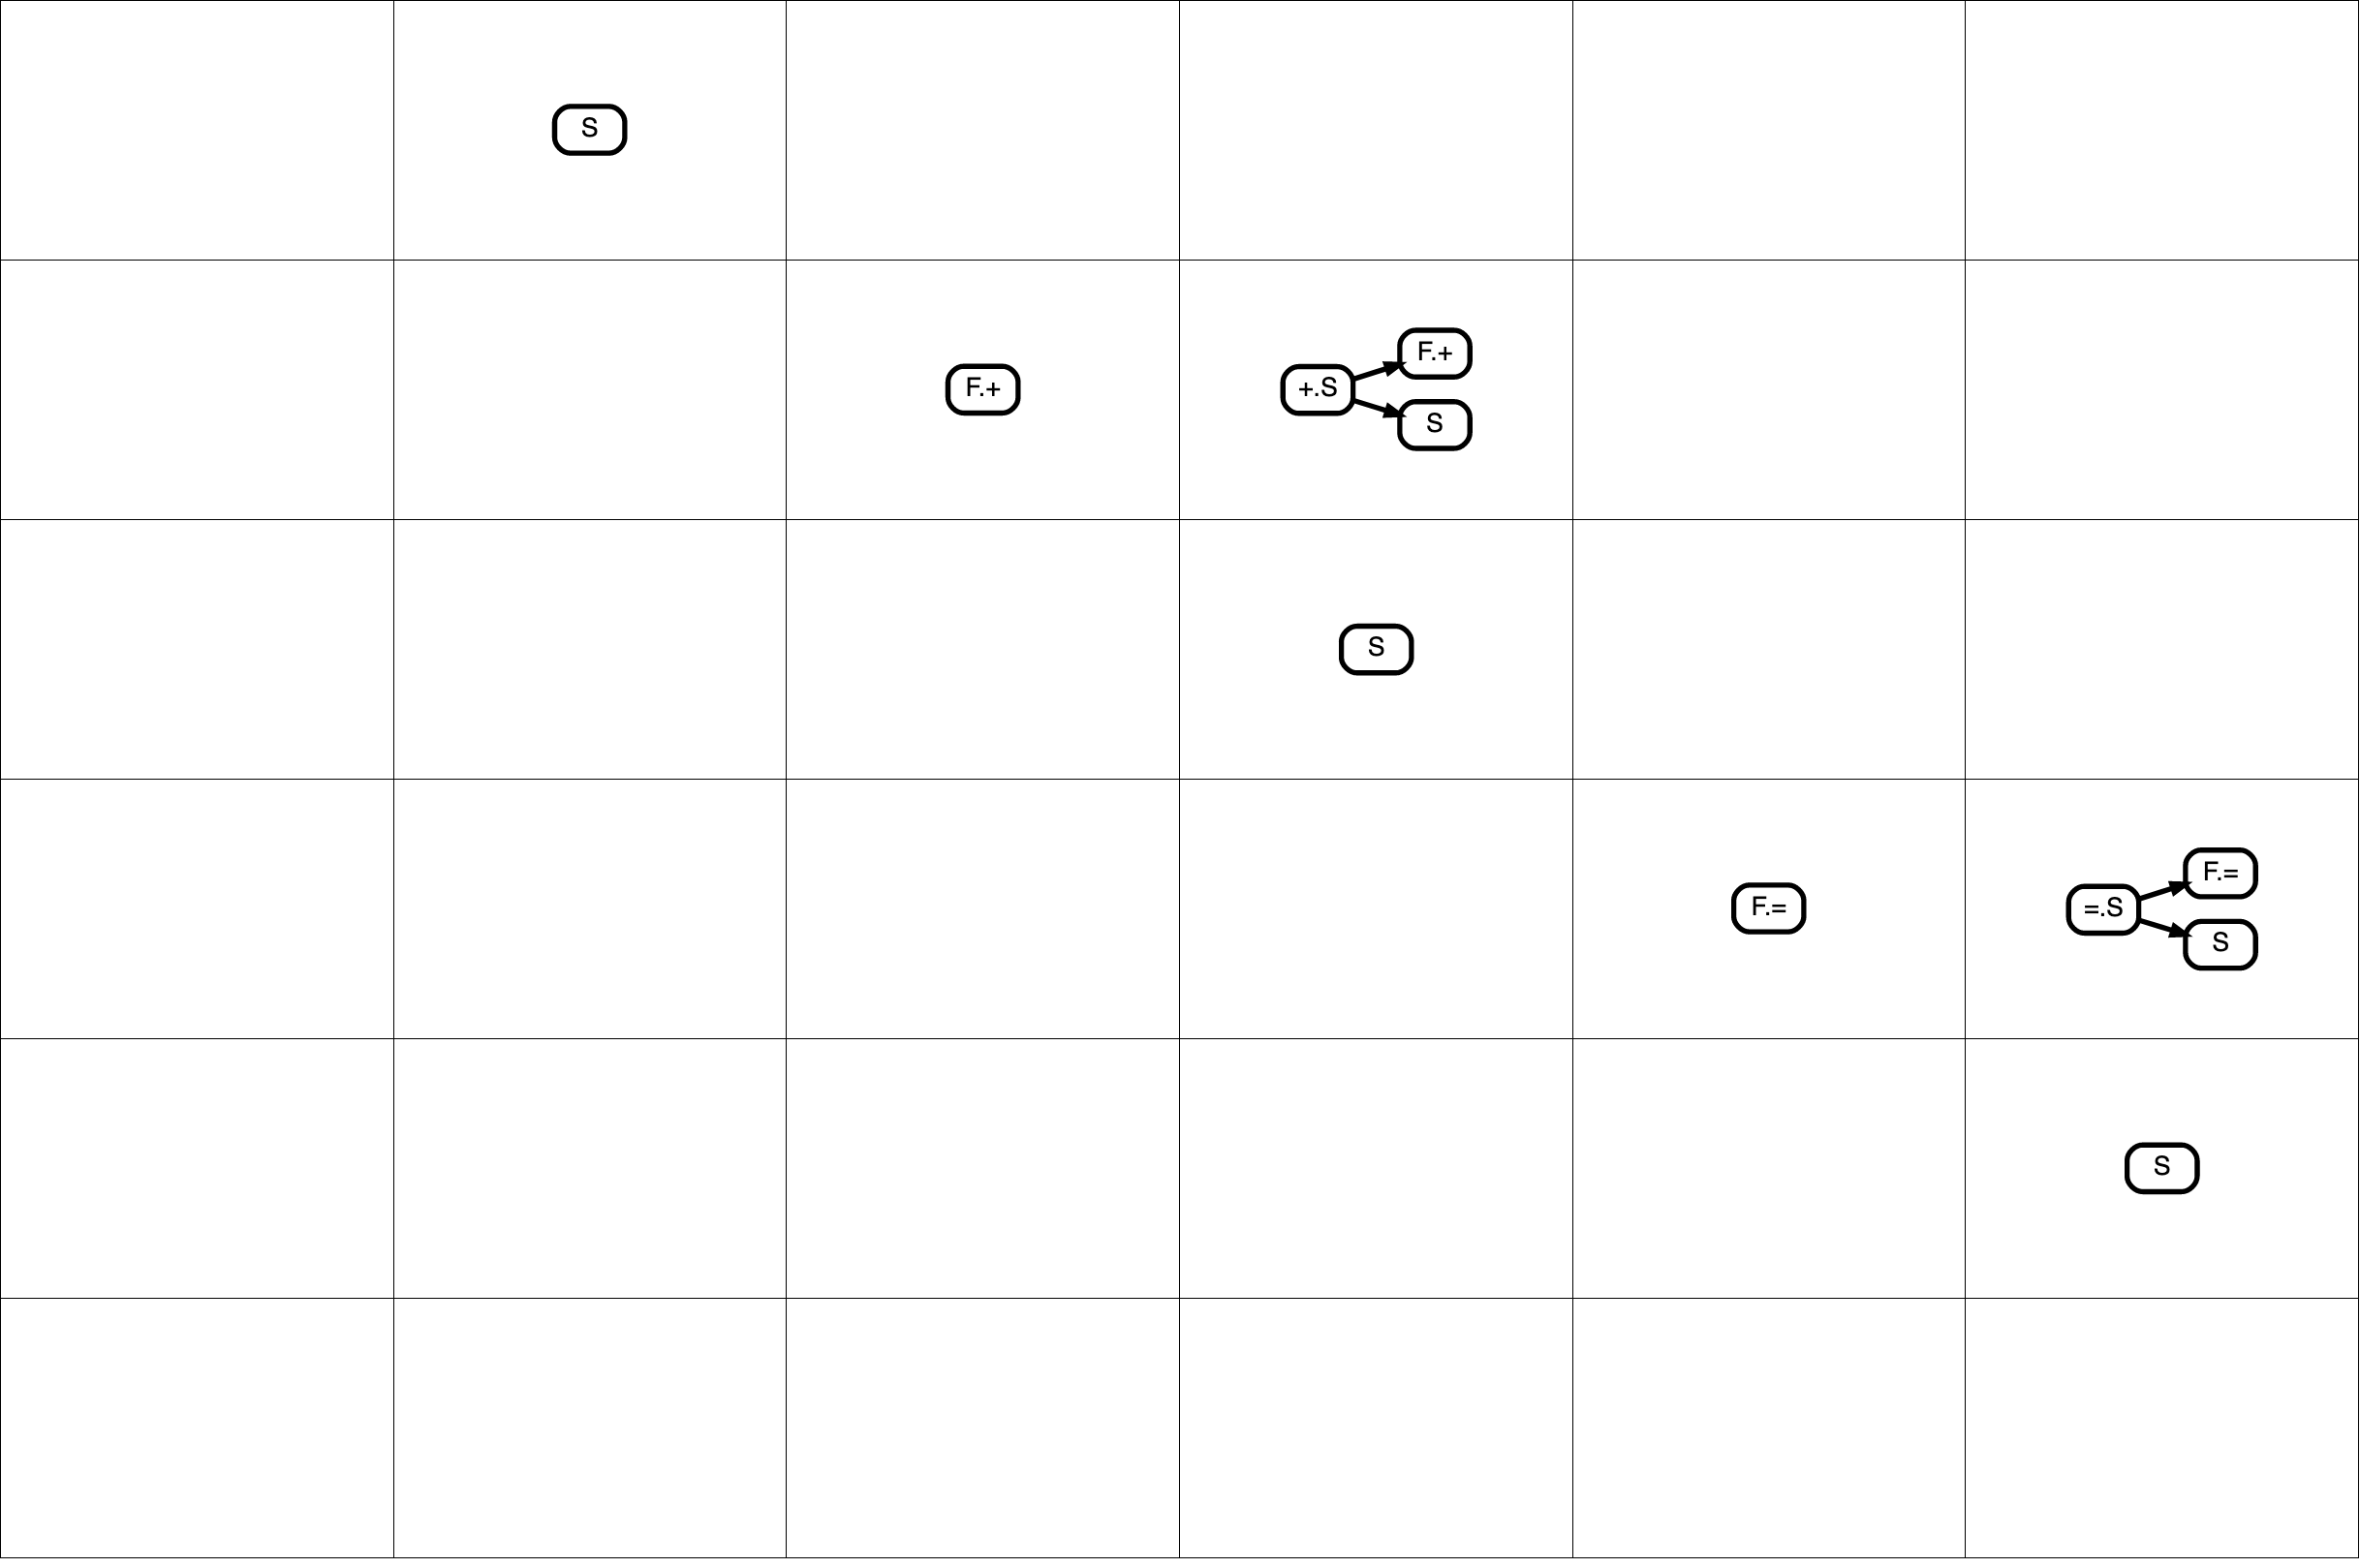
\includegraphics[width=2cm]{../figures/parse2.png}
%%    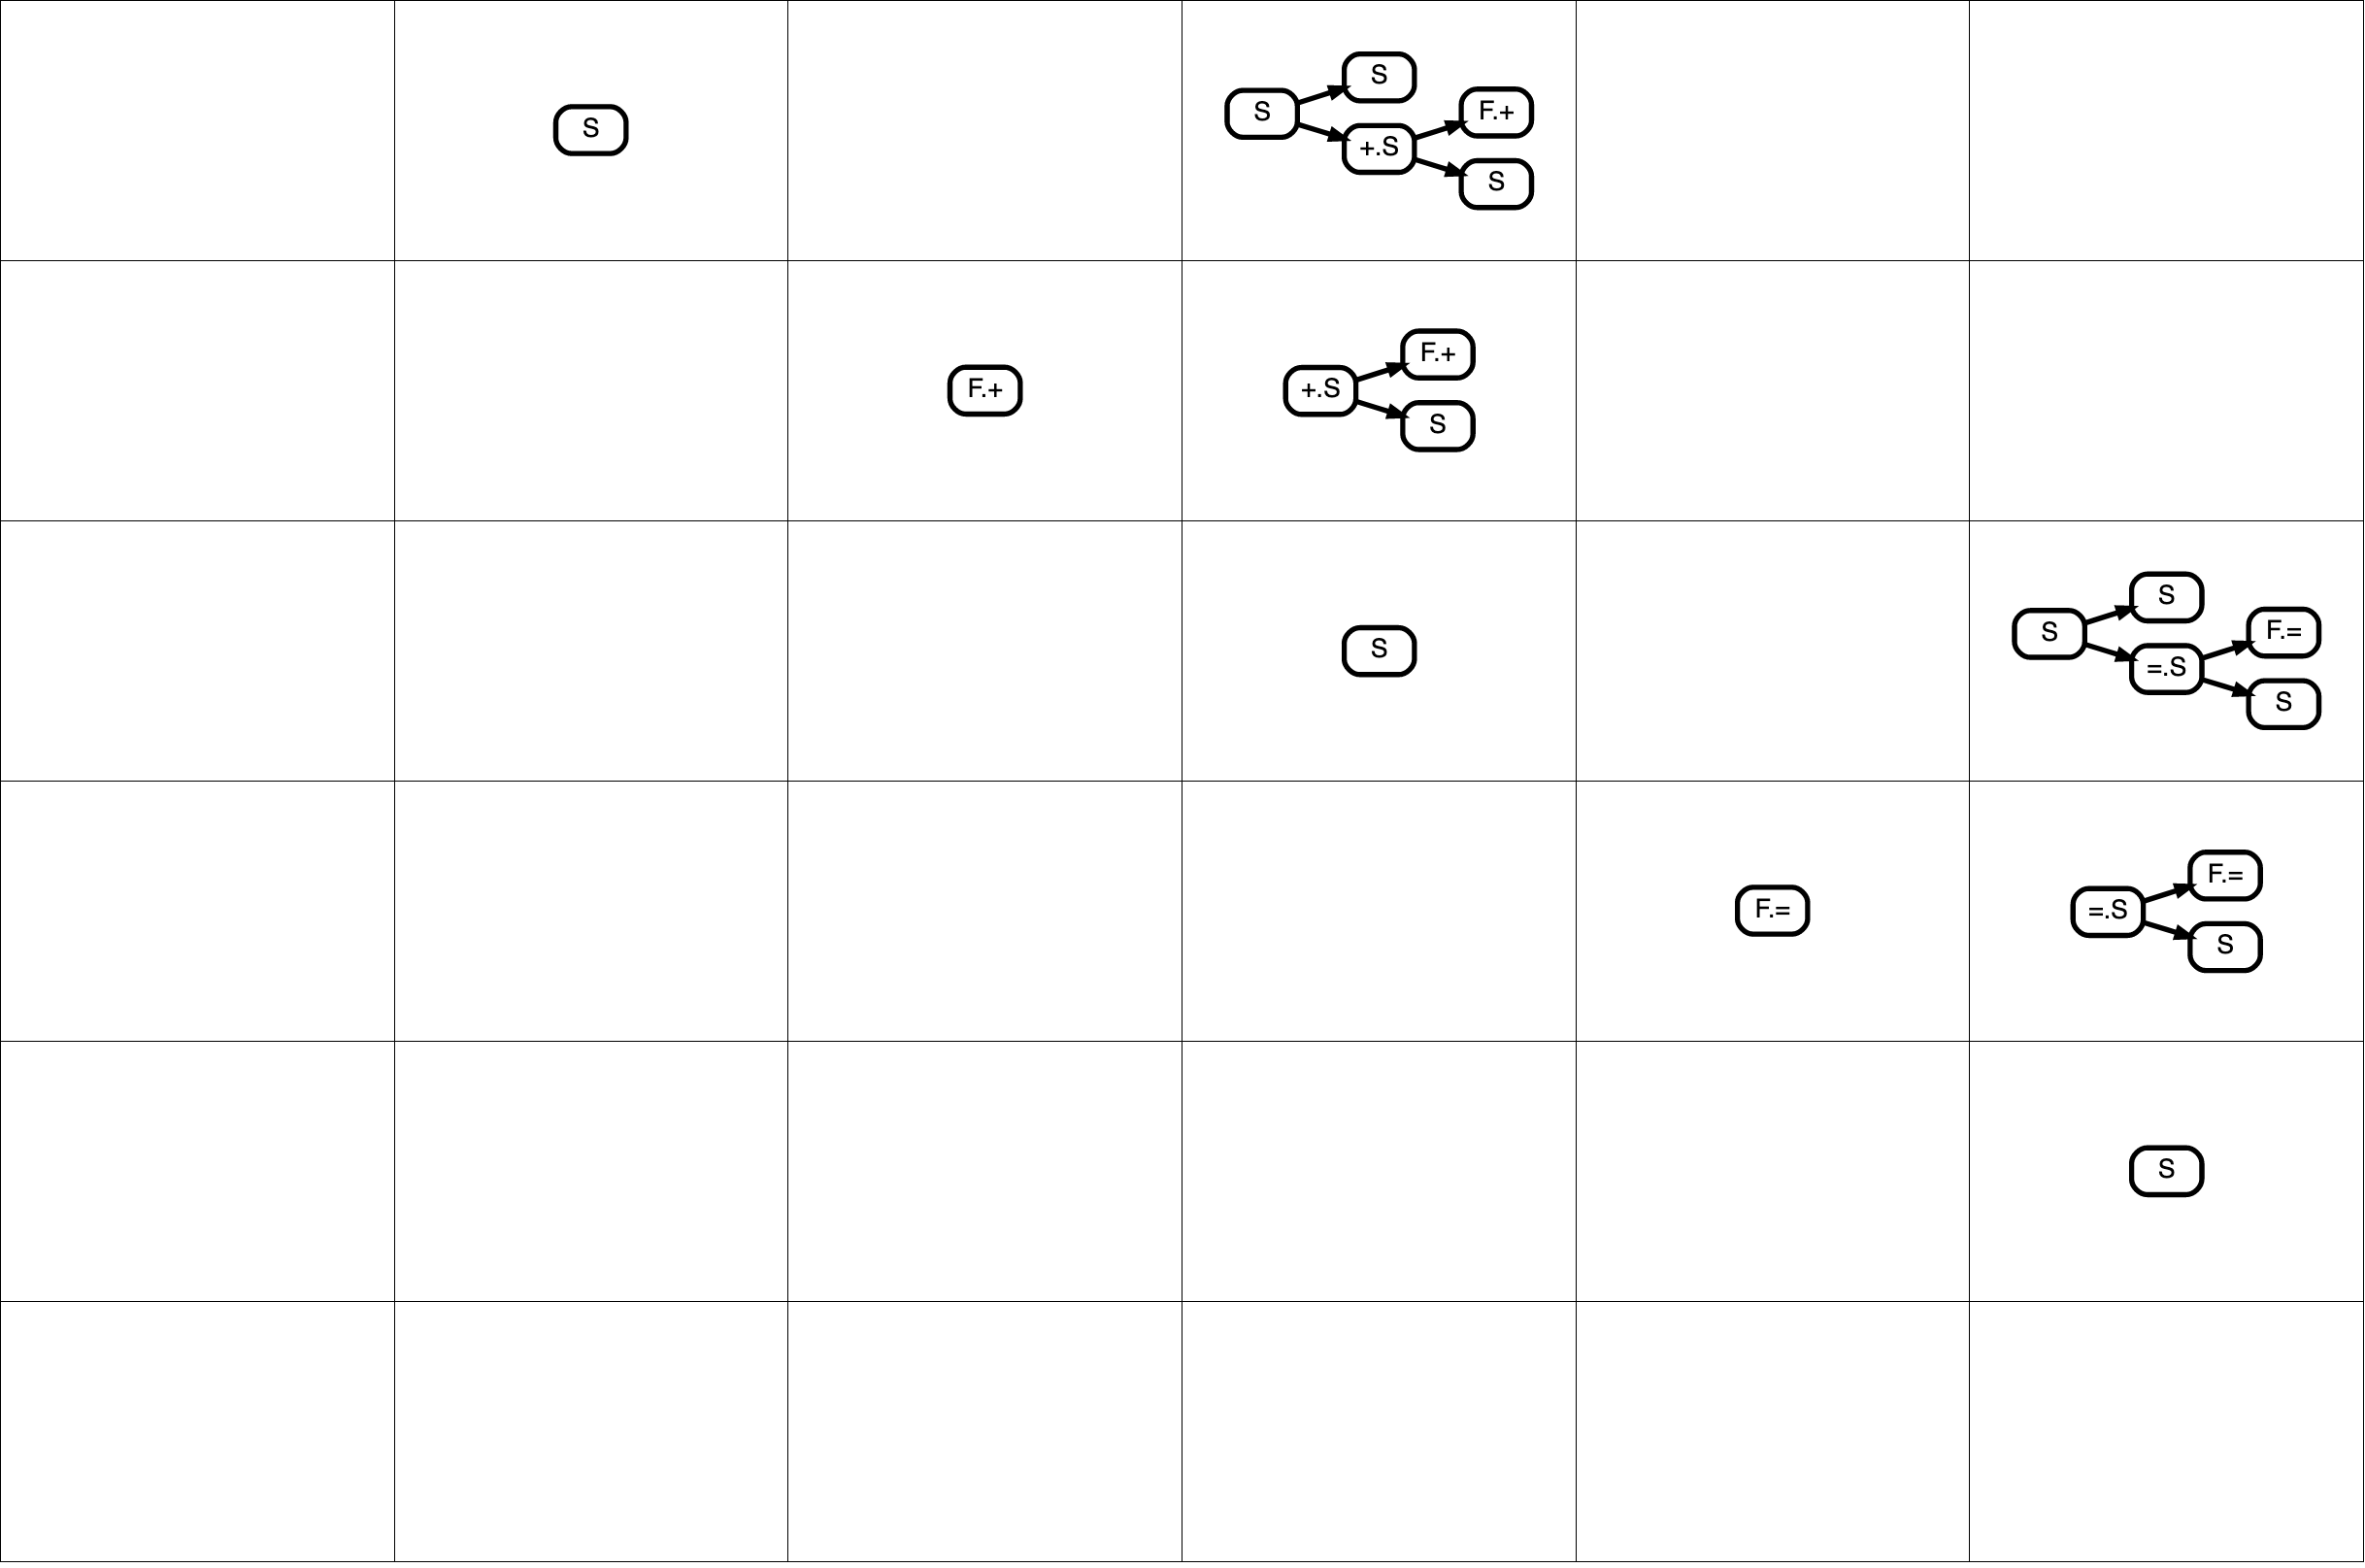
\includegraphics[width=2cm]{../figures/parse3.png}
%%    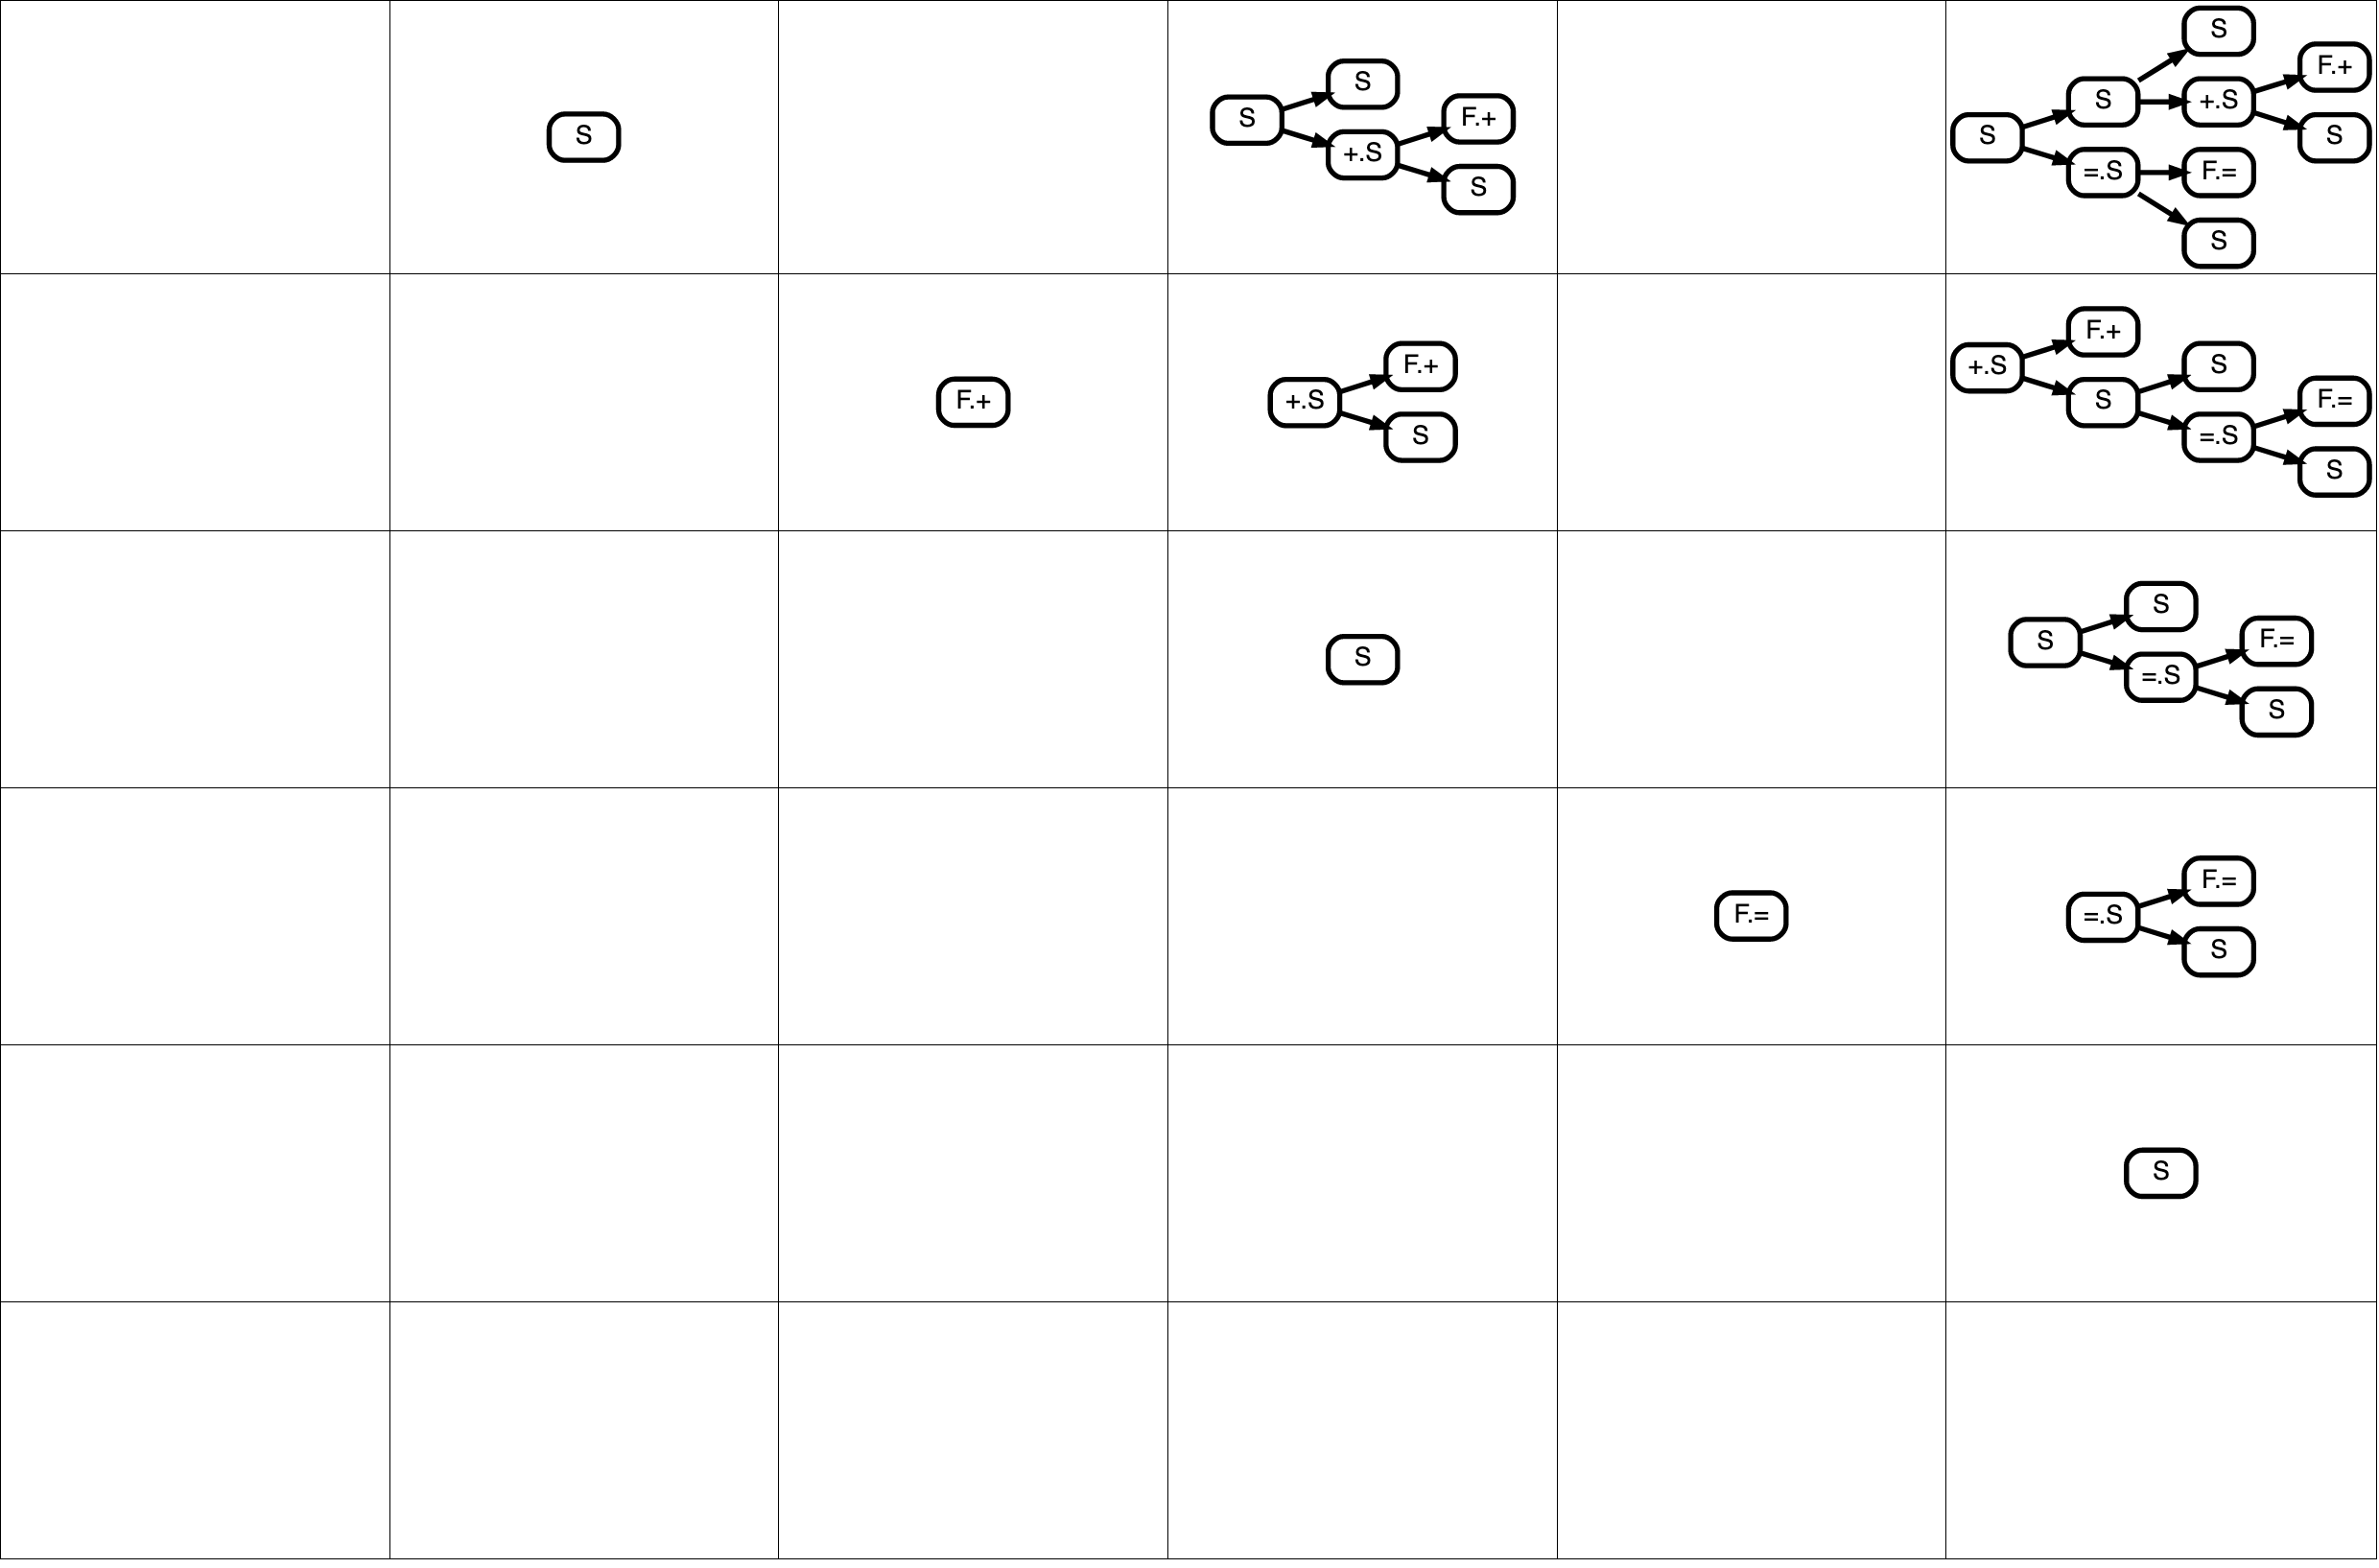
\includegraphics[width=2cm]{../figures/parse4.png}
%%\end{figure}
%
%  \begin{figure}[H]
%    \[
%      \mathcal{M}^* = \begin{pNiceArray}{ccccccc}[margin, extra-margin=2pt,colortbl-like, xdots/line-style=loosely dotted]
%          \vno & \rcr \shup x_1 &  \Cdots      & \mathcal{V}_{1,|x|} & \rcw \mathcal{V}_{1,4} & \cdd & \mathcal{V}^* \\
%          \vdd & \ddd           &  \Ddots      & \rcr\Vdots          & \rcw\vdd               &      & \vdd \\
%               &                &              & \rcr\shup x_{|x|}   & \rcw                   &      & \\
%               &                &              &                     & \mathcal{V}_{4,4}      &      & \\
%               &                &              &                     &                        & \ddd & \\
%               &                &              &                     &                        &      & \mathcal{V}_{n,n} \\
%          \vno & \cdd           &              &                     &                        &      & \vno
%      \end{pNiceArray}
%    \]
%  \end{figure}

%We also need the constraint that no two conflicting nonterminals may be active at any given time... TODO: describe uniqueness constraint
%  \noindent Depicted above is a SAT tensor representing \hlgray{$\sigma_1\:\sigma_2\:\sigma_3$}$\:\_\:\ldots\:\_$ where shaded regions demarcate known bitvector literals $\mathcal{L}_{r,c}$ (i.e., representing established nonterminal forests) and unshaded regions correspond to bitvector variables $\mathcal{V}_{r,c}$ (i.e., representing seeded nonterminal forests to be grown). Since $\mathcal{L}_{r,c}$ are fixed, we precompute them outside the SAT solver.

\pagebreak
\subsection{Gradient estimation}\label{sec:dsi}

Now that we have a reliable method to synthesize admissible completions for strings containing holes, i.e., fix \textit{localized} errors, $S: \mathcal{G} \times (\Sigma\cup\{\varepsilon, \texttt{\_}\})^n \rightarrow \{\Sigma^n\}\subseteq \mathcal{L}_\mathcal{G}$, how can we use $S$ to repair some unparseable string, i.e., $\err{\sigma_1\ldots\:\sigma_n}: \highlight{\Sigma}^n \cap\mathcal{L}_\mathcal{G}^\complement$ where the holes' locations are unknown? Three questions stand out in particular: how many holes are needed to repair the string, where should we put those holes, and how ought we fill them to obtain a parseable $\tilde{\sigma} \in \mathcal{L}_\mathcal{G}$?

One plausible approach would be to draw samples with a PCFG, minimizing tree-edit distance, however these are computationally expensive metrics and approximations may converge poorly. A more efficient strategy is to sample string perturbations, $\bm{\sigma}\sim\Sigma^{n\pm q}\cap\Delta_{q}(\err{\sigma})$, from the Levenshtein q-ball centered on $\err{\sigma}$, i.e., the space of all admissible edits with Levenshtein distance $\leq q$, loosely analogous to a finite difference approximation over words in a finite language.

To implement this strategy, we carefully construct a bijection between Levenshtein edits to a known string and the integers, sample integer vectors without replacement using a characteristic polynomial over a finite field, then decode vectors into repairs using a combinatorial indexing scheme that puts integer vectors into one-to-one correspondence with Levenshtein edits. We find this approach computationally more tractable while yielding a steady stream of admissible edits throughout the solving process, regardless of the grammar or string under repair.

More specifically, we employ a pair of [un]tupling functions $\kappa, \rho: \mathbb{N}^k \leftrightarrow \mathbb{N}$ which are (1) bijective (2) maximally compact (3) computationally tractable (i.e., closed form inverses). $\kappa$ will be used to index $\stirlingii{n}{k}$\footnote[2]{\text{We use the notation $\stirlingii{n}{d}$ to denote the set of all $d$-element subsets of $\{1,\ldots, n\}$.}}-combinations via the Maculay representation. $\rho$ will index $\Sigma^k$ tuples, but is slightly more tricky to define. To maximize compactness, there is an elegant pairing function courtesy of Szudzik~\cite{szudzik2006elegant}, which enumerates concentric square shells over the plane $\mathbb{N}^2$ and can be generalized to hypercubic shells in $\mathbb{N}^k$. For our purposes, this generalization will suffice.

Although $\langle\kappa, \rho\rangle$ could be used directly to exhaustively search the Levenshtein hypersphere, they are temporally biased samplers. Rather, we would prefer a path that uniformly visits every fertile subspace of the Levenshtein hypersphere over time regardless of the grammar or string in question: subsequences of $\langle\kappa, \rho\rangle$ should discover valid repairs with frequency roughly proportional to the ratio of admissible edits over all possible edits within a fixed distance of the original string. These additional constraints give rise to two more criteria: (1) ergodicity and (2) periodicity.

To achieve ergodicity, we permute the elements of $\stirlingii{n}{k}\times\Sigma^k$ using a finite field with a characteristic polynomial $C$ of degree $m:=\lceil \log_p {n \choose k}|\Sigma|^k \rceil$. By choosing $C$ to be some irreducible polynomial, one ensures the path is fully periodic while guaranteeing the mixing properties we desire, i.e., suppose $U: \mathbb{Z}_2^{m\times m}$ is a matrix whose structure is shown in Eq.~\ref{eq:lfsr}, wherein $C$ is a primitive polynomial over $\mathbb{Z}_2^m$ with coefficients $C_{1\ldots m}$ and semiring operators $\oplus := \veebar, \otimes := \land, \top := 1, \circ:=0$.\vspace{-5pt}

\begin{align}
    U^tV = \begin{pNiceMatrix}[nullify-dots,xdots/line-style=loosely dotted]
               C_1    & \cdd  &       &       & C_m \\
               \top   & \circ & \cdd  &       & \circ \\
               \circ  & \ddd  & \ddd  &       & \vdd \\
               \vdd   & \ddd  &       &       & \\
               \circ  & \cdd  & \circ & \top  & \circ
    \end{pNiceMatrix}^t
    \begin{pNiceMatrix}[nullify-dots,xdots/line-style=loosely dotted]
        V_1 \\
        \vdd\\
        \\
        \\
        V_m
    \end{pNiceMatrix}\label{eq:lfsr}
\end{align}

\noindent Since $C$ is primitive, the sequence $\mathbf{S} = (U^{0 \ldots 2^m-1}V)$ must have \textit{full periodicity}, i.e., for all $i, j \in[0, 2^m)$, ${\mathbf{S}_i = \mathbf{S}_j \Rightarrow i = j}$. To uniformly sample $\bm\sigma$ without replacement, we form an injection $\mathbb{Z}_2^m\rightharpoonup\stirlingii{n}{d}\times\Sigma_\varepsilon^{2d}$ using a combinatorial number system, cycle over $\mathbf{S}$, then discard samples which have no witness in $\stirlingii{n}{d}\times\Sigma_\varepsilon^{2d}$. This requires $\widetilde{\mathcal O}(1)$ per sample and $\widetilde{\mathcal O}\left({n \choose d}|\Sigma + 1|^{2d}\right)$ to exhaustively search $\stirlingii{n}{d}\times\Sigma_\varepsilon^{2d}$.

In addition to its statistically desirable properties, our sampler has the practical benefit of being trivially parallelizable using the leapfrog method, i.e., given $p$ independent processors, each one can independently check $\langle\kappa, \rho\rangle^{-1}(\mathbf{S}_{i}) \in \mathcal{L}(\mathcal{G})?$ where $i \equiv p_j \pmod p$. This procedure linearly scales with the number of processors, exhaustively searching $\Delta_{q}(\err{\sigma})$ in $p^{-1}$ of the time required by a single processor, or alternately drawing $p$ times as many samples in the same amount of time.

To admit variable-length edits, we first define a $\varepsilon^+$-production and introduce it to the right- and left-hand side of each terminal in a unit production:\vspace{5pt}

\begin{prooftree}
  \AxiomC{$\mathcal{G} \vdash \varepsilon \in \Sigma$}
  \RightLabel{$\varepsilon\textsc{-dup}$}
  \UnaryInfC{$\mathcal{G} \vdash (\varepsilon^+ \rightarrow \varepsilon \mid \varepsilon\:\varepsilon^+) \in P$}
  \DisplayProof
  \hskip 1.5em
  \AxiomC{$\mathcal{G} \vdash (A \rightarrow B) \in P$}
  \RightLabel{$\varepsilon^+\textsc{-int}$}
  \UnaryInfC{$\mathcal{G} \vdash (A \rightarrow B\:\varepsilon^+ \mid \varepsilon^+\:B \mid B) \in P$}
\end{prooftree}

Finally, to sample $\bm{\sigma}\sim\Delta_{q}(\err{\sigma})$, we enumerate templates $H(\sigma, i) = \sigma_{1\ldots i-1}\:\text{\_ \_}\:\sigma_{i+1\ldots n}$ for each $i \in \cdot \in \stirlingii{n}{d}$ and $d \in 1\ldots q$, then solve for $\mathcal{M}_{\bm\sigma}^*$. If $S \in \Lambda^*_{\bm\sigma}?$ has a solution, each edit in each $\tilde{\sigma} \in \bm\sigma$ will match one of the following seven patterns:\vspace{-10pt}

\begin{align*}
    \text{Deletion}&=\begin{cases}
                         \,\ldots\sigma_{i-1}\:\text{\hlred{$\gamma_1$}\:\hlred{$\gamma_2$}}\:\sigma_{i+1}\ldots\hspace{0.2cm}\gamma_{1, 2} = \varepsilon\label{eq:del}
    \end{cases}\\
    \text{Substitution}&=\begin{cases}
                             \ldots\sigma_{i-1}\:\text{\hlorange{$\gamma_1$}\:\hlred{$\gamma_2$}}\:\sigma_{i+1}\ldots\hspace{0.2cm}\gamma_1 \neq \varepsilon \land \gamma_2 = \varepsilon\\
                             \ldots\sigma_{i-1}\:\text{\hlred{$\gamma_1$}\:\hlorange{$\gamma_2$}}\:\sigma_{i+1}\ldots\hspace{0.2cm}\gamma_1 = \varepsilon \land \gamma_2 \neq \varepsilon\\
                             \ldots\sigma_{i-1}\:\text{\hlorange{$\gamma_1$}\:\hlorange{$\gamma_2$}}\:\sigma_{i+1}\ldots\hspace{0.2cm}\{\gamma_1, \gamma_2\}\cap\{\varepsilon, \sigma_i\} = \varnothing
    \end{cases}\\
    \text{Insertion}&=\begin{cases}
                          \ldots\sigma_{i-1}\:\text{\hlgreen{$\gamma_1$}\:\hlorange{$\gamma_2$}}\:\sigma_{i+1}\ldots\hspace{0.2cm}\gamma_1 = \sigma_i \land \gamma_2 \notin \{\varepsilon,  \sigma_i\}\label{eq:ins2}\\
                          \ldots\sigma_{i-1}\:\text{\hlorange{$\gamma_1$}\:\hlgreen{$\gamma_2$}}\:\sigma_{i+1}\ldots\hspace{0.2cm}\gamma_1 \notin \{\varepsilon, \sigma_i\} \land \gamma_2 = \sigma_i\label{eq:ins1}\\
                          \ldots\sigma_{i-1}\:\text{\hlgreen{$\gamma_1$}\:\hlgreen{$\gamma_2$}}\:\sigma_{i+1}\ldots\hspace{0.2cm}\gamma_{1,2} = \sigma_i\label{eq:copy}
    \end{cases}
\end{align*}

\noindent This approach is tractable for $n \lesssim 100, q \lesssim 3$, however more complex repairs require a more efficient gradient estimator. We will discuss two alternate approaches, one using an adaptive sampler (Sec.~\ref{sec:holes}) and another based on Levenshtein reachability (Sec.~\ref{sec:levenshtein}).

\pagebreak\section{Probabilistic reachability}\label{sec:holes}

Since there are $\Sigma_{d=1}^q{n \choose d}$ total sketch templates, each with $(|\Sigma| + 1)^{2d}$ individual edits to check, if $n$ and $q$ are large, this space can be intractable to exhaustively search and a uniform prior may be highly sample-inefficient. Furthermore, na\"ively sampling $\bm{\sigma}_i\sim\Sigma^{n\pm q}\cap\Delta_{q}(\err{\sigma})$ is likely to produce a large number of unnatural edits. To provide rapid and relevant suggestions, we prioritize candidate repairs according to the following seven-step procedure:

\begin{enumerate}
    \item Retrieve the most recent grammar, $\mathcal{G}$, and string, $\err{\sigma}$, from the editor.
%    \item Lazily enumerate edit templates, $i_{1\ldots d} \in \stirlingii{n}{d}$, for increasing values of $d \geq 1$.
%    \item Rerank edit templates according to the distribution $\int\mathcal{F}_\theta(\cdot \mid i_{1\ldots d})d\theta$.
    \item Sample completions for each template from $\bm{\sigma}_i\sim \stirlingii{n}{d}\times\Sigma^{n\pm q}\cap\Delta_{q}(\err{\sigma})$ WoR using Eq.~\ref{eq:lfsr}.
    \item Filter completions by admissibility with respect to the grammar, $\bm{\sigma}_i \cap \mathcal{L}_{\mathcal{G}}$.
    \item Rerank admissible repairs by the edit cost model, $C(\err{\sigma}, \tilde{\sigma})$.
    \item Display the top-k repairs by edit cost found within p-seconds to the user.
\end{enumerate}

Suppose we are given an invalid string, $\err{\sigma}: \Sigma^{90}$ and $\mathcal{F}_\theta$, a distribution over possible edits locations provided by a probabilistic or neural language model, which we can use to localize admissible repairs. For example, by marginalizing onto $\err{\sigma}$, the distribution $\mathcal{F}_\theta$ could take the following form:

\begin{figure}[H]
    \hspace{-0.3cm}\begin{tikzpicture}[scale=0.4]
        \begin{axis}[x=2cm, y=2cm, every axis plot post/.append style={mark=none,domain=-2:7.5,samples=50,smooth},
            axis x line*=bottom, % no box around the plot, only x and y axis
            ticks=none,
            y axis line style={draw=none},
            xticklabels={,,},
            enlargelimits=upper] % extend the axes a bit to the right and top
            \addplot[name path=F] {gauss(0.0,0.4)};
            \addplot[name path=G] {gauss(3.0,0.5)};
            \addplot[name path=H] {gauss(6.0,0.3)};
            \addplot[name path=N] {nil(0)};
            \addplot[pattern=vertical lines, pattern color=gray!50]fill between[of=F and N, soft clip={domain=-3:1}];
            \addplot[pattern=vertical lines, pattern color=gray!50]fill between[of=G and N, soft clip={domain=1:5}];
            \addplot[pattern=vertical lines, pattern color=gray!50]fill between[of=H and N, soft clip={domain=4:7.5}];
        \end{axis}
        \node [xshift=4.1cm, yshift=-7pt] {\footnotesize $\sigma_1\hspace{0.5cm}\sigma_{10}\err{\hspace{0.5cm}\sigma_{20}}\hspace{0.5cm}\sigma_{30}\hspace{0.5cm}\err{\sigma_{40}\hspace{0.5cm}\sigma_{50}}\hspace{0.5cm}\sigma_{60}\hspace{0.5cm}\err{\sigma_{70}\hspace{0.3cm}}\hspace{0.2cm}\sigma_{80}\hspace{0.5cm}\sigma_{90}$};
%  \node [xshift=142pt, yshift=7pt] {\footnotesize $P_2(X)$};
%  \node [xshift=227pt, yshift=7pt] {\footnotesize $P_3(X)$};
    \end{tikzpicture}
    \caption{The distribution $\int\mathcal{F}_{\theta}(\cdot \mid i_{1\ldots d})d\theta$, projected onto the invalid string, suggests edit locations most likely to yield admissible repairs, from which we draw subsets of size $d$.}
\end{figure}

Morally, we would prefer sketch templates likely to yield repairs that are (1) admissible (i.e., grammatically correct) and (2) plausible (i.e., likely to have been written by a human author). To do so, we draw holes and rank admissible repairs using a distance metric over $\Delta_q(\err{\sigma})$. One such metric, the Kantorovich--Rubinstein (KR) metric, $\delta_{KR}$, can be viewed as an optimal transport problem minimizing $\Pi(\mu, \nu)$, the set of all mass-conserving transportation plans between two probability distributions $\mu$ and $\nu$ over a metric space $\Omega$:

\begin{align}
    \delta_{\textsc{KR}}(\mu, \nu) := \inf_{\pi\in \Pi(\mu, \nu)}\int_{\Omega\times \Omega} \delta(x, y)d\pi(x, y)
\end{align}

More specifically in our setting, $\Omega$ is a discrete product space that factorizes into (1) the specific edit locations (e.g., informed by caret position, historical edit locations, or a static analyzer), (2) probable completions (e.g., from a Markov chain or neural language model) and (3) an accompanying \textit{cost model}, $C: (\Sigma^* \times \Sigma^*) \rightarrow \mathbb{R}$, which may be any number of suitable distance metrics, such as language edit distance, finger travel distance on a physical keyboard, weighted Levenshtein distance, or stochastic contextual edit distance~\cite{cotterell+al.acl14} in the case of probabilistic edits. Our goal then, is to discover repairs which minimize $C(\err{\sigma}, \tilde{\sigma})$, subject to the given grammar and latency constraints.

In the following section, we will give a more efficient construction for generating and accepting $\Delta_{q}(\err{\sigma})$ that incorporates (1) and (3), but does not explicitly require enumerating hole configurations.%As SAT encoding incurs a fixed penalty, for small repairs, we have observed it is more efficient to enumerate all sketch templates and solve for admissible repairs outside the SAT solver.

%  This constitutes to a top-down inference procedure, in which, following the tradition of Bird and Meertens, we define the exponential of a forest as a nested datatype called a \textit{taiga}:
%
%  \begin{align*}
%    \text{\textbf{data} \textit{Tree} } a &= \varnothing \mid \langle a, \langle\textit{Tree a, Tree a}\rangle\rangle\\
%    \text{\textbf{data} \textit{Forest} } a &= \varnothing \mid \langle \{a\}, \{\langle\textit{Forest a,  Forest a}\rangle\}\rangle\\
%    \text{\textbf{data} \textit{Taiga} } a &= \varnothing \mid \langle a, [\langle\textit{Taiga (Taiga a)}\rangle^2]\rangle
%  \end{align*}
%
%  This is needed because of the doubly-ambiguous nature of tree search: a single string may have a parse forest, and an incomplete string simultaneously occupies a superposition of possible parse forests. When we encounter two adjacent parse forests which cannot be joined, we know that either (1) the left derivation must change (2) the right derivation must change or (3) there must be a hole in the middle which joins the two together. When recursing over the state space, we must simultaneously consider all three possibilities.

\pagebreak
\section{Levenshtein reachability}\label{sec:levenshtein}

Levenshtein reachability is recognized by the nondeterministic infinite automaton (NIA) whose topology $\mathcal{L} = \knightkingarrow$ can be factored into a product of (a) the monotone Chebyshev topology $\kingarrow$, equipped with horizontal transitions accepting $\sigma_{i}$ and vertical transitions accepting Kleene stars, and (b) the monotone knight's topology $\knightarrow$, equipped with transitions accepting $\sigma_{i+2}$. The structure of this space is representable as an acyclic NFA~\cite{schulz2002fast}, populated by accept states within radius $k$ of $q_{n,0}$, or equivalently, a left-linear CFG whose productions finitely instantiate the transition dynamics:

\begin{figure}[H]
\begin{minipage}[c]{0.45\textwidth}
\centering
\underline{NFA}\vspace{10pt}
\resizebox{\textwidth}{!}{
\begin{tikzpicture}[
%->, % makes the edges directed
>=stealth',
node distance=2.5cm, % specifies the minimum distance between two nodes. Change if necessary.
%  every state/.style={thick, fill=gray!10}, % sets the properties for each ’state’ node
initial text=$ $, % sets the text that appears on the start arrow
]
\node[state, initial]                (00) {$q_{0,0}$};
\node[state, right of=00]            (10) {$q_{1,0}$};
\node[state, right of=10]            (20) {$q_{2,0}$};
\node[state, right of=20]            (30) {$q_{3,0}$};
\node[right of=30]                   (40) {$\vphantom{\vdots}\cdots$};
\node[accepting, state, right of=40] (n0) {$q_{n,0}$};

\node[state, above of=00]            (01) {$q_{0,1}$};
\node[state, right of=01]            (11) {$q_{1,1}$};
\node[state, right of=11]            (21) {$q_{2,1}$};
\node[state, right of=21]            (31) {$q_{3,1}$};
\node[right of=31]                   (41) {$\vphantom{\vdots}\cdots$};
\node[accepting, state, right of=41] (n1) {$q_{n,1}$};

\node[above of=01]                   (0j) {$\mathmakebox[\widthof{$\cdots$}]{\vdots}$};
\node[right of=0j]                   (1j) {$\mathmakebox[\widthof{$\cdots$}]{\vdots}$};
\node[right of=1j]                   (2j) {$\mathmakebox[\widthof{$\cdots$}]{\vdots}$};
\node[right of=2j]                   (3j) {$\mathmakebox[\widthof{$\cdots$}]{\vdots}$};
\node[right of=3j]                   (4j) {$\iddots$};
\node[accepting, right of=4j]        (nj) {$\mathmakebox[\widthof{$\cdots$}]{\vdots}$};

\node[state, above of=0j]            (0k) {$q_{0,k}$};
\node[state, right of=0k]            (1k) {$q_{1,k}$};
\node[state, right of=1k]            (2k) {$q_{2,k}$};
\node[state, right of=2k]            (3k) {$q_{3,k}$};
\node[right of=3k]                   (4k) {$\vphantom{\vdots}\cdots$};
\node[accepting, state, right of=4k] (nk) {$q_{n,k}$};

\draw [->] (00) edge[below] node{$\sigma_1$}    (10);
\draw [->] (10) edge[below] node{$\sigma_2$}    (20);
\draw [->] (20) edge[below] node{$\sigma_3$}    (30);
\draw [->] (30) edge[below] node{$\sigma_4$}              (40);
\draw [->] (40) edge[below] node{$\sigma_n$}    (n0);

\draw [->] (01) edge[below] node{$\sigma_1$}    (11);
\draw [->] (11) edge[below] node{$\sigma_2$}    (21);
\draw [->] (21) edge[below] node{$\sigma_3$}    (31);
\draw [->] (31) edge[below] node{$\sigma_4$}              (41);
\draw [->] (41) edge[below] node{$\sigma_n$}    (n1);

\draw [->] (0j) edge[below] node{$\sigma_1$}    (1j);
\draw [->] (1j) edge[below] node{$\sigma_2$}    (2j);
\draw [->] (2j) edge[below] node{$\sigma_3$}    (3j);
\draw [->] (3j) edge[below] node{$\sigma_4$}              (4j);
\draw [->] (4j) edge[below] node{$\sigma_n$}    (nj);

\draw [->] (0k) edge[below] node{$\sigma_1$}    (1k);
\draw [->] (1k) edge[below] node{$\sigma_2$}    (2k);
\draw [->] (2k) edge[below] node{$\sigma_3$}    (3k);
\draw [->] (3k) edge[below] node{$\sigma_4$}              (4k);
\draw [->] (4k) edge[below] node{$\sigma_n$}    (nk);

\draw [->] (00) edge[left] node{$*$}            (11);
\draw [->] (10) edge[left] node{$*$}            (21);
\draw [->] (20) edge[left] node{$*$}            (31);
\draw [->] (30) edge[left] node{$*$}            (41);
\draw [->] (30) edge[bend right, below] node{$\sigma_5$}            (41);
\draw [->] (40) edge[           right] node{$\sigma_n$}            (n1);
\draw [->] (40) edge[bend right, left] node{$*$}            (n1);

\draw [->] (01) edge[left] node{$*$}            (1j);
\draw [->] (11) edge[left] node{$*$}            (2j);
\draw [->] (21) edge[left] node{$*$}            (3j);
\draw [->] (31) edge[left] node{$*$}            (4j);
\draw [->] (31) edge[bend right, below] node{$\sigma_5$}            (4j);
\draw [->] (41) edge[           right] node{$\sigma_n$}            (nj);
\draw [->] (41) edge[bend right, left] node{$*$}            (nj);

\draw [->] (0j) edge[left] node{$*$}            (1k);
\draw [->] (1j) edge[left] node{$*$}            (2k);
\draw [->] (2j) edge[left] node{$*$}            (3k);
\draw [->] (3j) edge[left] node{$*$}            (4k);
\draw [->] (3j) edge[bend right, below] node{$\sigma_5$}            (4k);
\draw [->] (4j) edge[           right] node{$\sigma_n$}            (nk);
\draw [->] (4j) edge[bend right, left] node{$*$}            (nk);

\draw [->] (00) edge[bend left, left] node{$*$} (01);
\draw [->] (10) edge[bend left, left] node{$*$} (11);
\draw [->] (20) edge[bend left, left] node{$*$} (21);
\draw [->] (30) edge[bend left, left] node{$*$} (31);
\draw [->] (40) edge[right] node{$*$} (41);
\draw [->] (n0) edge[bend right, right] node{$*$} (n1);

\draw [->] (01) edge[bend left, left] node{$*$} (0j);
\draw [->] (11) edge[bend left, left] node{$*$} (1j);
\draw [->] (21) edge[bend left, left] node{$*$} (2j);
\draw [->] (31) edge[bend left, left] node{$*$} (3j);
\draw [->] (41) edge[right] node{$*$} (4j);
\draw [->] (n1) edge[bend right, right] node{$*$} (nj);

\draw [->] (0j) edge[bend left, left] node{$*$} (0k);
\draw [->] (1j) edge[bend left, left] node{$*$} (1k);
\draw [->] (2j) edge[bend left, left] node{$*$} (2k);
\draw [->] (3j) edge[bend left, left] node{$*$} (3k);
\draw [->] (4j) edge[right] node{$*$} (4k);
\draw [->] (nj) edge[bend right, right] node{$*$} (nk);

\draw [->] (00) edge[below] node{$\sigma_2$}    (21);
\draw [->] (10) edge[below] node{$\sigma_3$}    (31);
\draw [->] (20) edge[below] node{$\sigma_4$}    (41);

\draw [->] (01) edge[below] node{$\sigma_2$}    (2j);
\draw [->] (11) edge[below] node{$\sigma_3$}    (3j);
\draw [->] (21) edge[below] node{$\sigma_4$}    (4j);

\draw [->] (0j) edge[below] node{$\sigma_2$}    (2k);
\draw [->] (1j) edge[below] node{$\sigma_3$}    (3k);
\draw [->] (2j) edge[below] node{$\sigma_4$}    (4k);

%https://tex.stackexchange.com/a/20986/139648
\draw [decorate,decoration={brace,amplitude=10pt,raise=10pt,mirror}] (00.south west) -- (n0.south east) node[midway,yshift=-3em]{\textbf{String length}};
\draw [decorate,decoration={brace,amplitude=10pt,raise=20pt}] (00.south west) -- (0k.north west) node[midway,xshift=-40pt,rotate=90]{\textbf{Levenshtein edit distance}};
\end{tikzpicture}
}
\end{minipage}
\hfill
\begin{minipage}[l]{5 cm}
\centering
\underline{CFG}\vspace{7pt}
\begin{align*}
S &\Rightarrow \{\cdot \in Q \mid \delta(\cdot, q_{n,0}) \leq k\}\\
* &\Rightarrow \{\cdot \in \Sigma\}\\
\big\{q_{i, j} &\Rightarrow \{q_{i, j-1}*\} \mid i, j \in [1, n]\times[1, k]\big\}\\
\big\{q_{i, j} &\Rightarrow \{q_{i-1, j-1}*\}\mid i, j\in[1, n]\times [1, k]\big\}\\
\big\{q_{i, j} &\Rightarrow \{q_{i-1, j} \sigma_i \}\mid i, j \in [1, n]\times[0, k]\big\} \\
\big\{q_{i, j} &\Rightarrow \{q_{i-2, j-1} \sigma_i\} \mid i, j \in [2, n]\times[1, k] \big\}\\
\end{align*}
\end{minipage}
\caption{Levenshtein reachability from $\Sigma^n$ can be described as either an acyclic $\epsilon$-free NFA, or a left-linear CFG.}
\end{figure}

\section{Language Edit Reachability}\label{sec:editreach}

\begin{wrapfigure}{r}{0.33\textwidth}
\begin{minipage}[c]{0.33\textwidth}
\centering
\resizebox{\textwidth}{!}{
\begin{tikzpicture}[
dot/.style = {circle, inner sep=0pt, minimum size=1mm, fill,
node contents={}}
]
\def\firstcircle{(-2.1,0) coordinate (a) circle (2.4cm)}
\def\firstcirclea{(-2.1,0) coordinate (b) circle (0.6cm)}
\def\firstcircleb{(-2.1,0) coordinate (c) circle (1.2cm)}
\def\firstcirclec{(-2.1,0) coordinate (d) circle (1.8cm)}
\def\secondcircle{(1.2,0) coordinate (e) circle (1.5cm)}
\begin{scope}
\clip \secondcircle;
\fill[black!15] \firstcircle;
\end{scope}
\draw \firstcircle node[dot,label=$\err{\sigma}$](z0);
\draw [dashed] \firstcirclea;
\draw [dashed] \firstcircleb;
\draw [dashed] \firstcirclec;
\draw[-stealth] (-2.1,0) -- (-1.5, 0) node[midway,below]{$d_1$};
\draw[-stealth] (-1.5,0) -- (-0.9, 0) node[midway,below]{$d_2$};
\draw[-stealth] (-0.9,0) -- (-0.3, 0) node[midway,below]{$\vphantom{d}\ldots$};
\draw[-stealth] (-0.3,0) -- (0.3, 0) node[midway,below]{$d^*$};
\draw[-stealth] (-0.3,0) -- (0.3, 0) node[midway,above]{$\tilde{\sigma}$};
\draw \secondcircle;
\node [above] at (current bounding box.north -| a) {$\mathcal{L}(G(\err\sigma, d^*))$};
\node [above,yshift=1.5cm] at (e) {$\mathcal{L}(\mathcal{G}')$};
\end{tikzpicture}
}
\end{minipage}
\caption{LED is computed gradually by incrementing $d$ until $\mathcal{L}^\cap_{d}\neq \varnothing$.}
\end{wrapfigure}

Assume a hypothetical $\Phi(\mathcal{G}': \mathbb{G}, \err{\sigma}: \Sigma^*)\mapsto \tilde{\sigma}: \mathcal{L}(\mathcal{G}')$ which takes a CFG, $\mathcal{G}'$, generating an arbitrary nonempty CFL, and an unparseable string, $\err{\sigma}$, and which returns element(s) of $\mathcal{L}(\mathcal{G}')$ most similar to $\err{\sigma}$ according to their Levenshtein distance $\Delta(\err{\sigma}, \cdot)$.

Let $G(\err{\sigma}: \Sigma^*, d: \mathbb{N}^+) \mapsto \mathbb{G}$ be the specific construction described in Sec.~\ref{sec:levenshtein} which accepts a string, $\err{\sigma}$, and an edit distance, $d$, and returns a grammar representing the NFA that recognizes the language of all strings within Levenshtein radius $d$ of $\err{\sigma}$. To find the language edit distance and corresponding least-distance edit, we must find the smallest $d$ such that $\mathcal{L}^\cap_d$ is nonempty, where $\mathcal{L}^\cap_d$ is defined as $\mathcal{L}(G(\err\sigma, d)) \cap \mathcal{L}(\mathcal{G}')$. In other words, we seek $\tilde{\sigma}$ and $d^*$ under which three criteria are equisatisfiable:\linebreak (1) $\tilde{\sigma}\in\mathcal{L}(\mathcal{G}')$, and (2) $\Delta(\err{\sigma}, \tilde{\sigma}) \leq d^* \Longleftrightarrow \tilde{\sigma} \in \mathcal{L}(G(\err{\sigma}, d^*))$, and (3) $\not\exists \sigma' \in \mathcal{L}(\mathcal{G}').[\Delta(\err{\sigma}, \sigma') < d^*]$.
To satisfy these criteria, it suffices to check $d \in (1, d_{\max}]$ by encoding the Levenshtein automata and the original grammar as a single SAT formula, call it, $\varphi_d(\cdot)$ and gradually admitting new acceptance states at increasing radii. If $\varphi_d(\cdot)$ returns UNSAT, $d$ is increased until either (1) a satisfying assignment is found or (2) $d_{\max}$ is attained. This procedure is guaranteed to terminate in at most either (1) the number of steps required to overwrite every symbol in $\err{\sigma}$, or (2) the length of the shortest string in $\mathcal{L}(\mathcal{G}')$, whichever is greater. More precisely:

\begin{equation}
\varphi_{d+1}(\mathcal{G}', \err{\sigma}) := \begin{cases}
\varphi[\tilde{\sigma}\in\mathcal{L}(G(\err\sigma, d)) \land \tilde{\sigma}\in \mathcal{L}(\mathcal{G}')] & \text{if $d=1$ or SAT}.\\
\varphi_{d} \oplus \bigoplus_{\{q \in Q \mid \delta(q, q_{n,0}) = d+1\}}\varphi[S \rightarrow q] & \text{if $d \leq \max(|\err{\sigma}|, \min_{\sigma \in \mathcal{L}(\mathcal{G}')}|\sigma|)$}.
\end{cases}
\end{equation}

\noindent The function $\varphi_{d+1}(\mathcal{G}', \err{\sigma})$ is a realizer of $\Phi$.

%By intersection with a CFG, $\mathcal{G}'$, Bar-Hillel ensures the resulting language will remain context-free.
%
%We then intersect that language with $\Sigma^n$ and $\mathcal{L}(\mathcal{G})$, the original grammar, to obtain a finite set.

\section{Linear conjunctive reachability}\label{sec:lclreach}

It is well-known that the family of CFLs is not closed under intersection. Let us consider the traditional example, $\mathcal{L}_\cap := \mathcal{L}(\mathcal{G}_1) \cap \mathcal{L}(\mathcal{G}_2)$ defined as follows:

\begin{table}[H]
\begin{tabular}{llll}
  $P_1 := \big\{\;S \rightarrow L\:R,$ & $\:L \rightarrow a\:b \mid a\:L\:b,$ & $R \rightarrow c \mid c \:R\;\big\}$\vspace{5pt}\\
  $P_2 := \big\{\;S \rightarrow L\:R,$ & $\:R \rightarrow b\:c \mid b\:R\:c,$ & $L \rightarrow a \mid a \:L\;\big\}$
\end{tabular}
\end{table}

\noindent Note that $\mathcal{L}_\cap$ generates the language $\big\{\;a^d b^d c^d \mid d > 0\;\big\}$, which according to the pumping lemma is not context-free. We can encode $\bigcap_{i=1}^c \mathcal{L}(\mathcal{G}_i)$ as a polygonal prism with upper-triangular matrices adjoined to each rectangular face. More precisely, we intersect all terminals $\Sigma_\cap := \bigcap_{i=1}^c \Sigma_i$, then for each $t_\cap \in \Sigma_\cap$ and CFG, construct an equivalence class $E(t_\cap, \mathcal{G}_i) = \{ w_i \mid (w_i \rightarrow t_\cap) \in P_i\}$ and bind them together using conjunction:\vspace{-5pt}

\begin{align}
  \bigwedge_{t\in\Sigma_\cap}\bigwedge_{j = 1}^{c-1}\bigwedge_{i=1}^{|\sigma|} E(t_{\cap}, \mathcal{G}_j) \equiv_{\sigma_i} E(t_{\cap}, \mathcal{G}_{j+1})
\end{align}
  % Generated by cfl4_intersection.vox, open with https://voxelator.com/
\begin{figure}[H]
  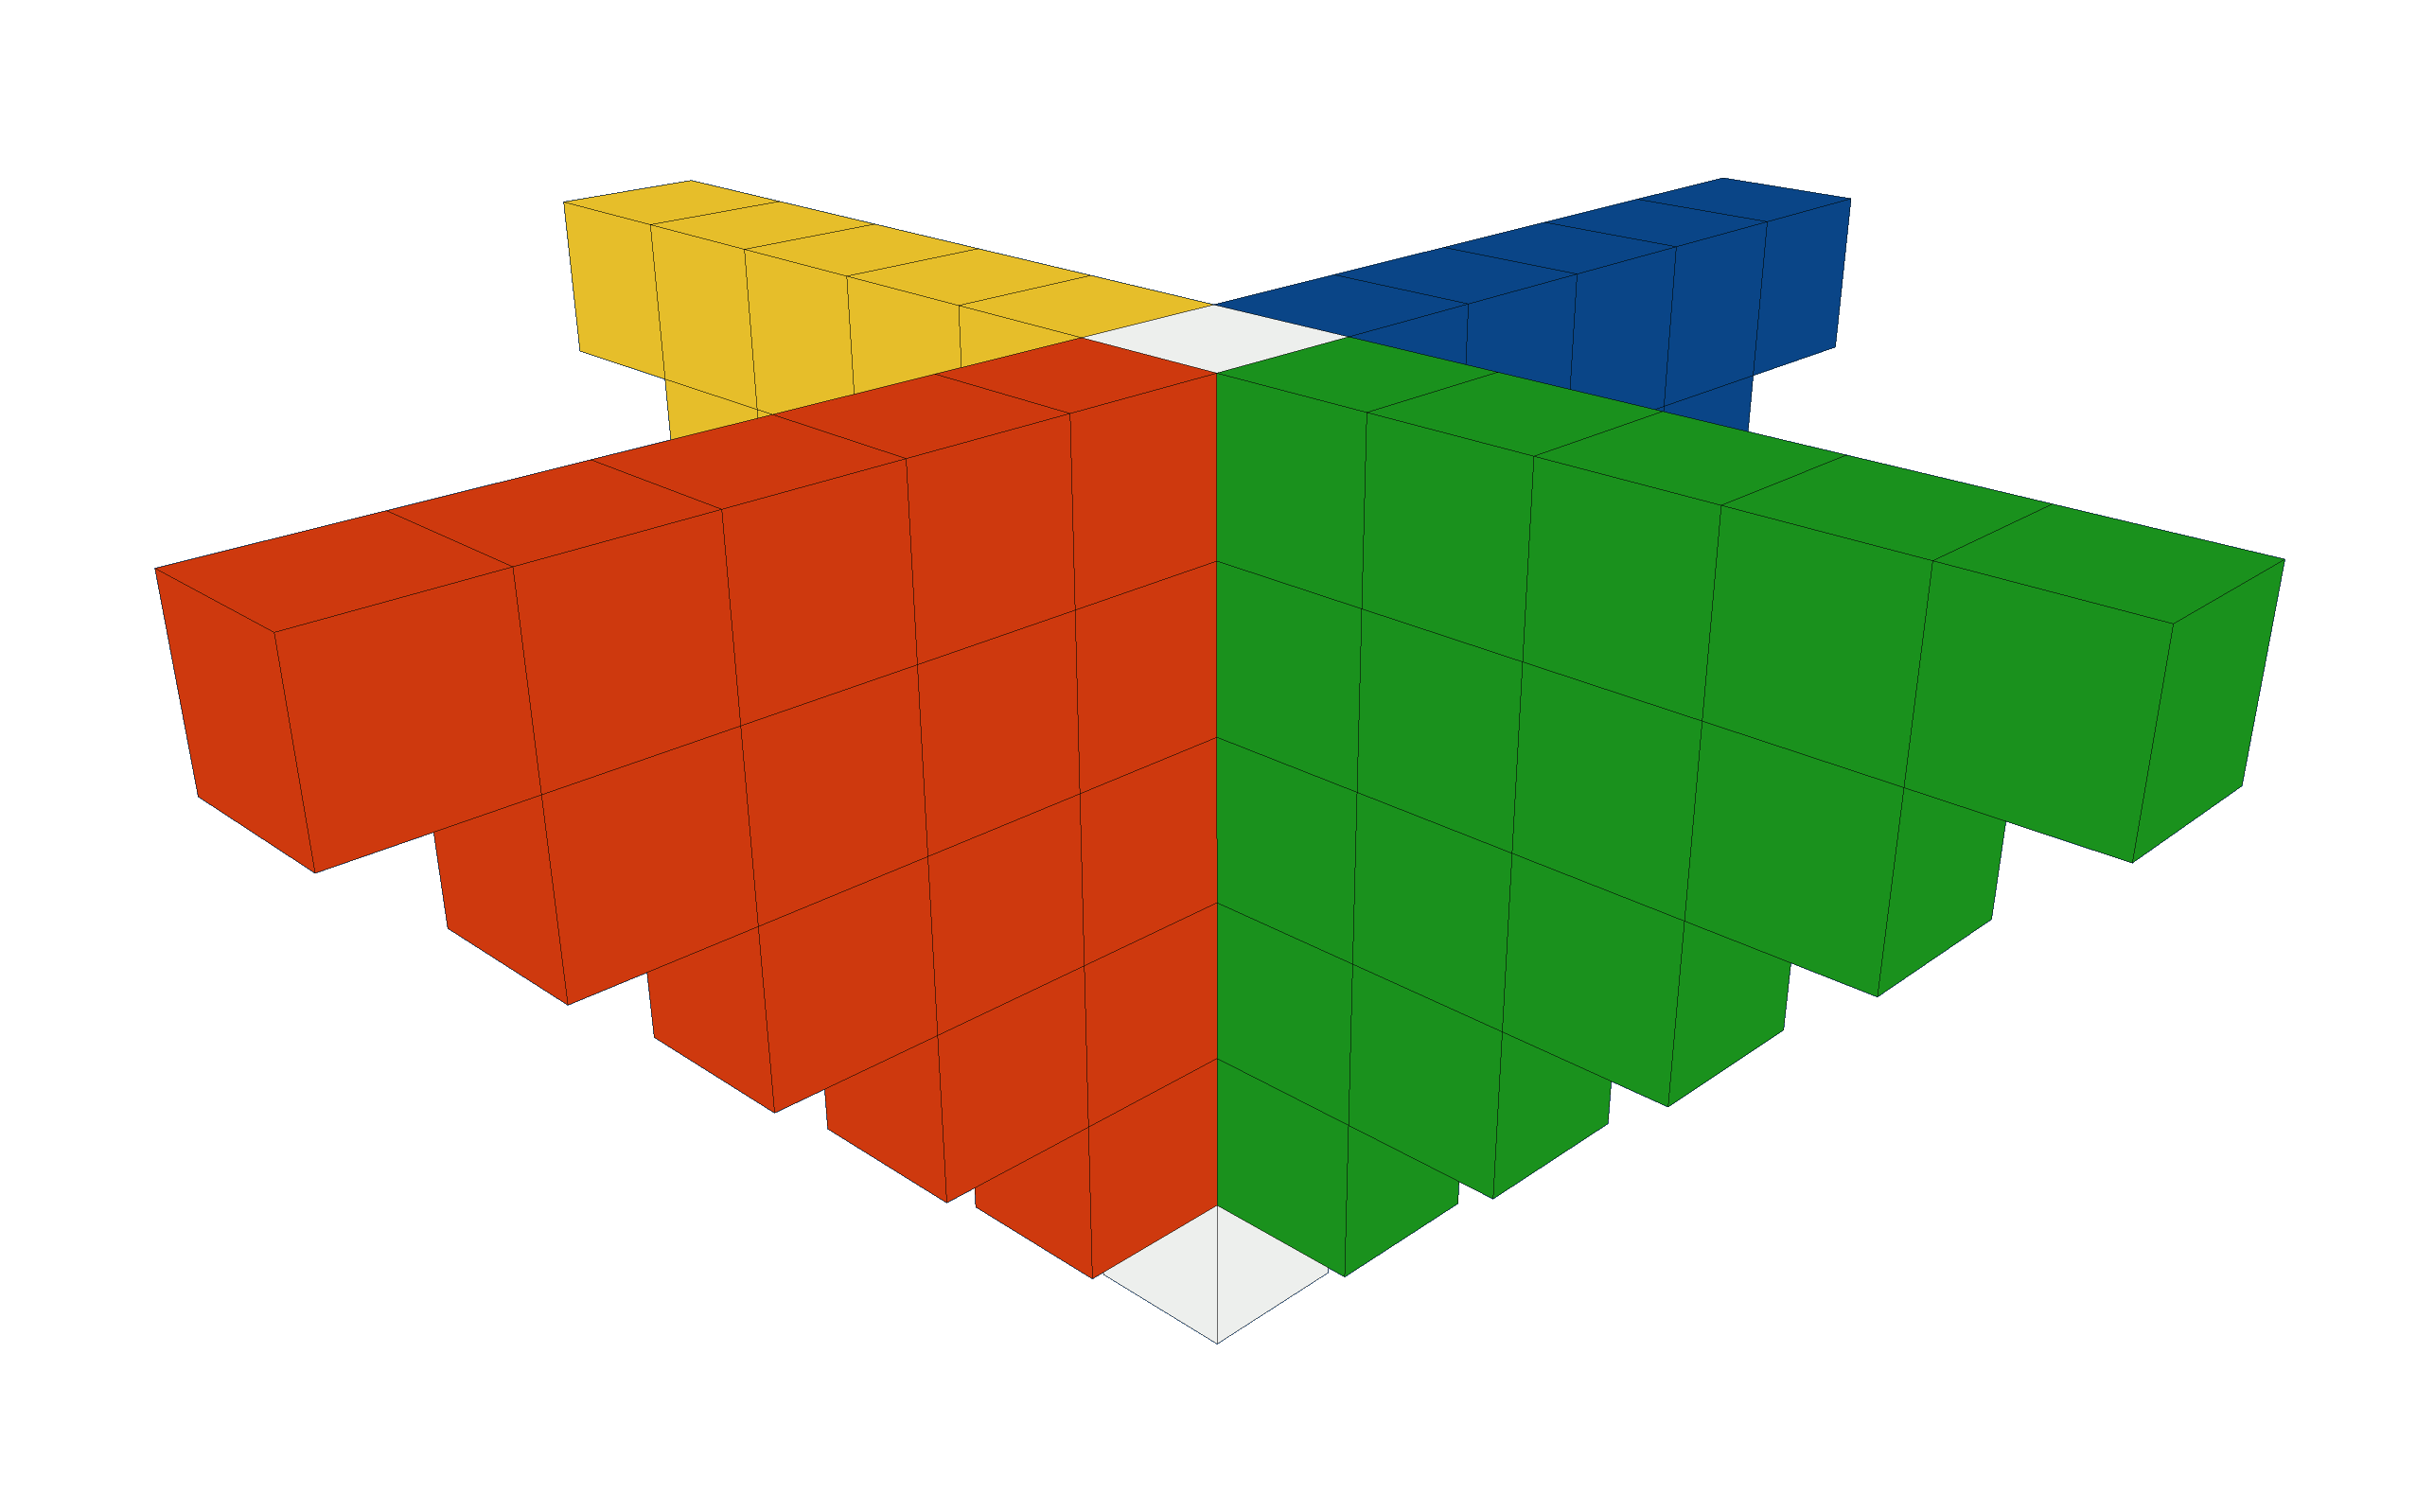
\includegraphics[height=0.1\textwidth]{../figures/angle1.png}\hspace{-5pt}
  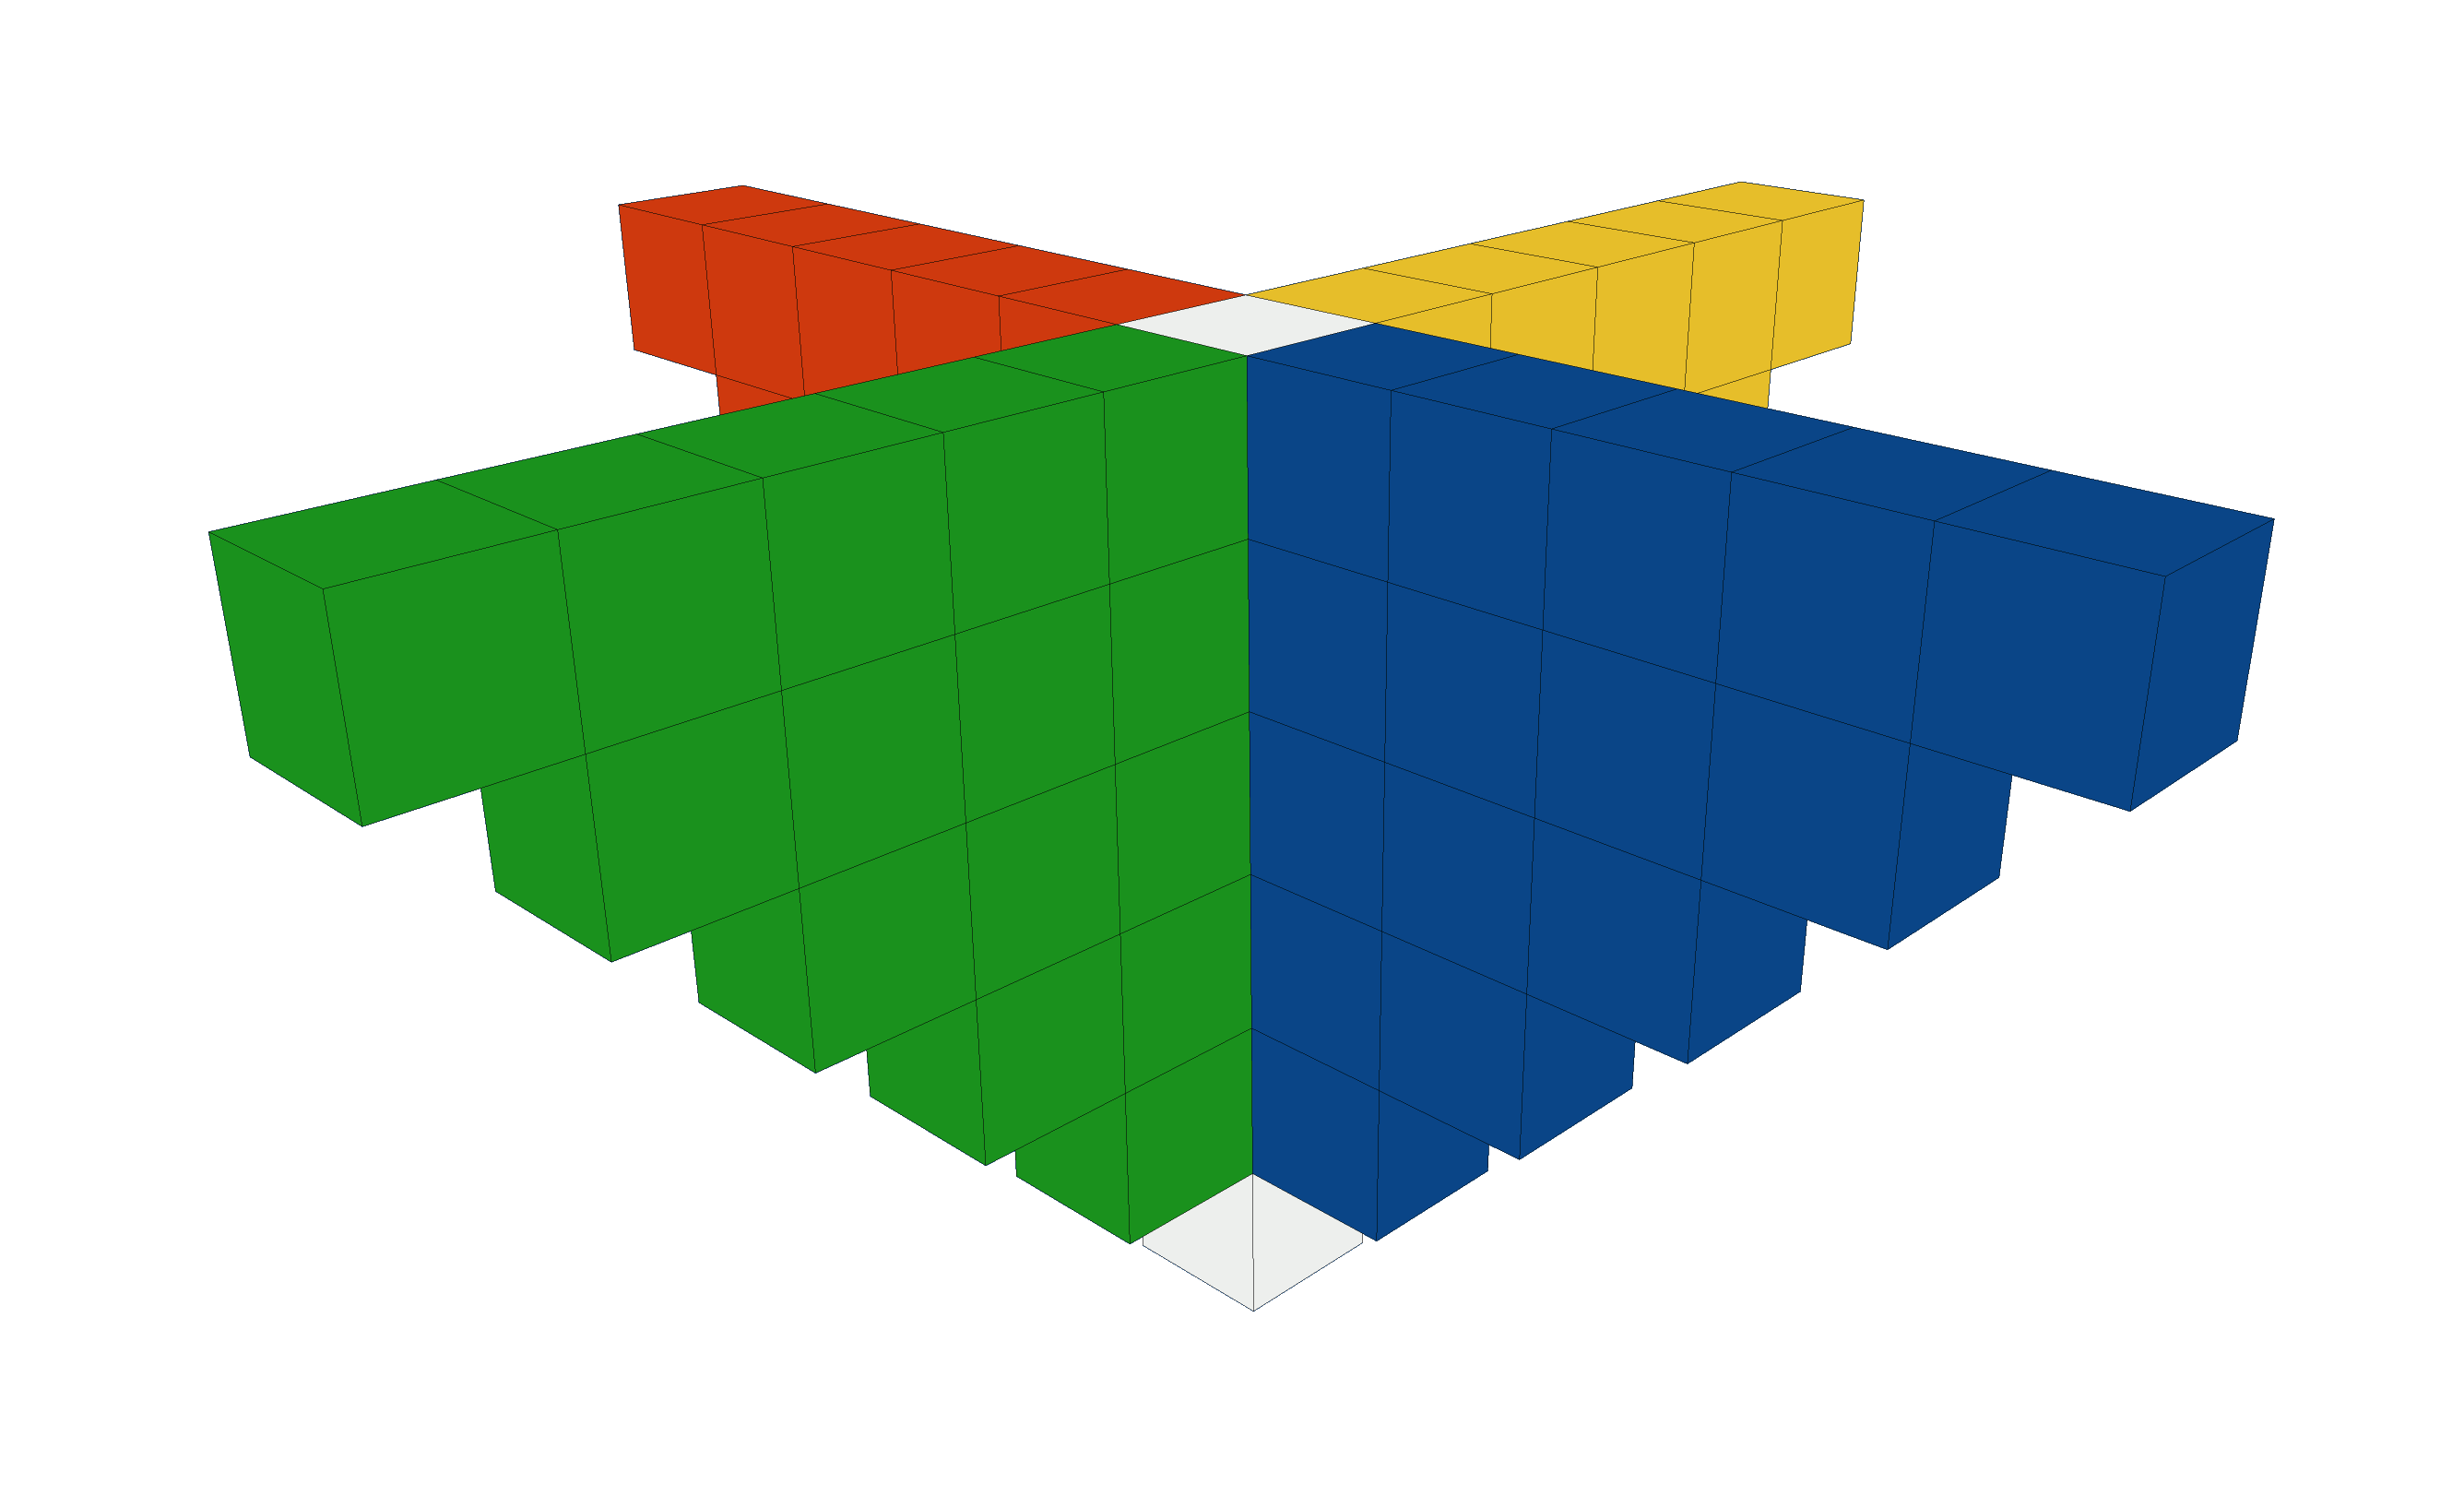
\includegraphics[height=0.1\textwidth]{../figures/angle2.png}\hspace{-5pt}
  
\includegraphics[height=0.1\textwidth]{../figures/angle5.png}\hspace{-5pt}
  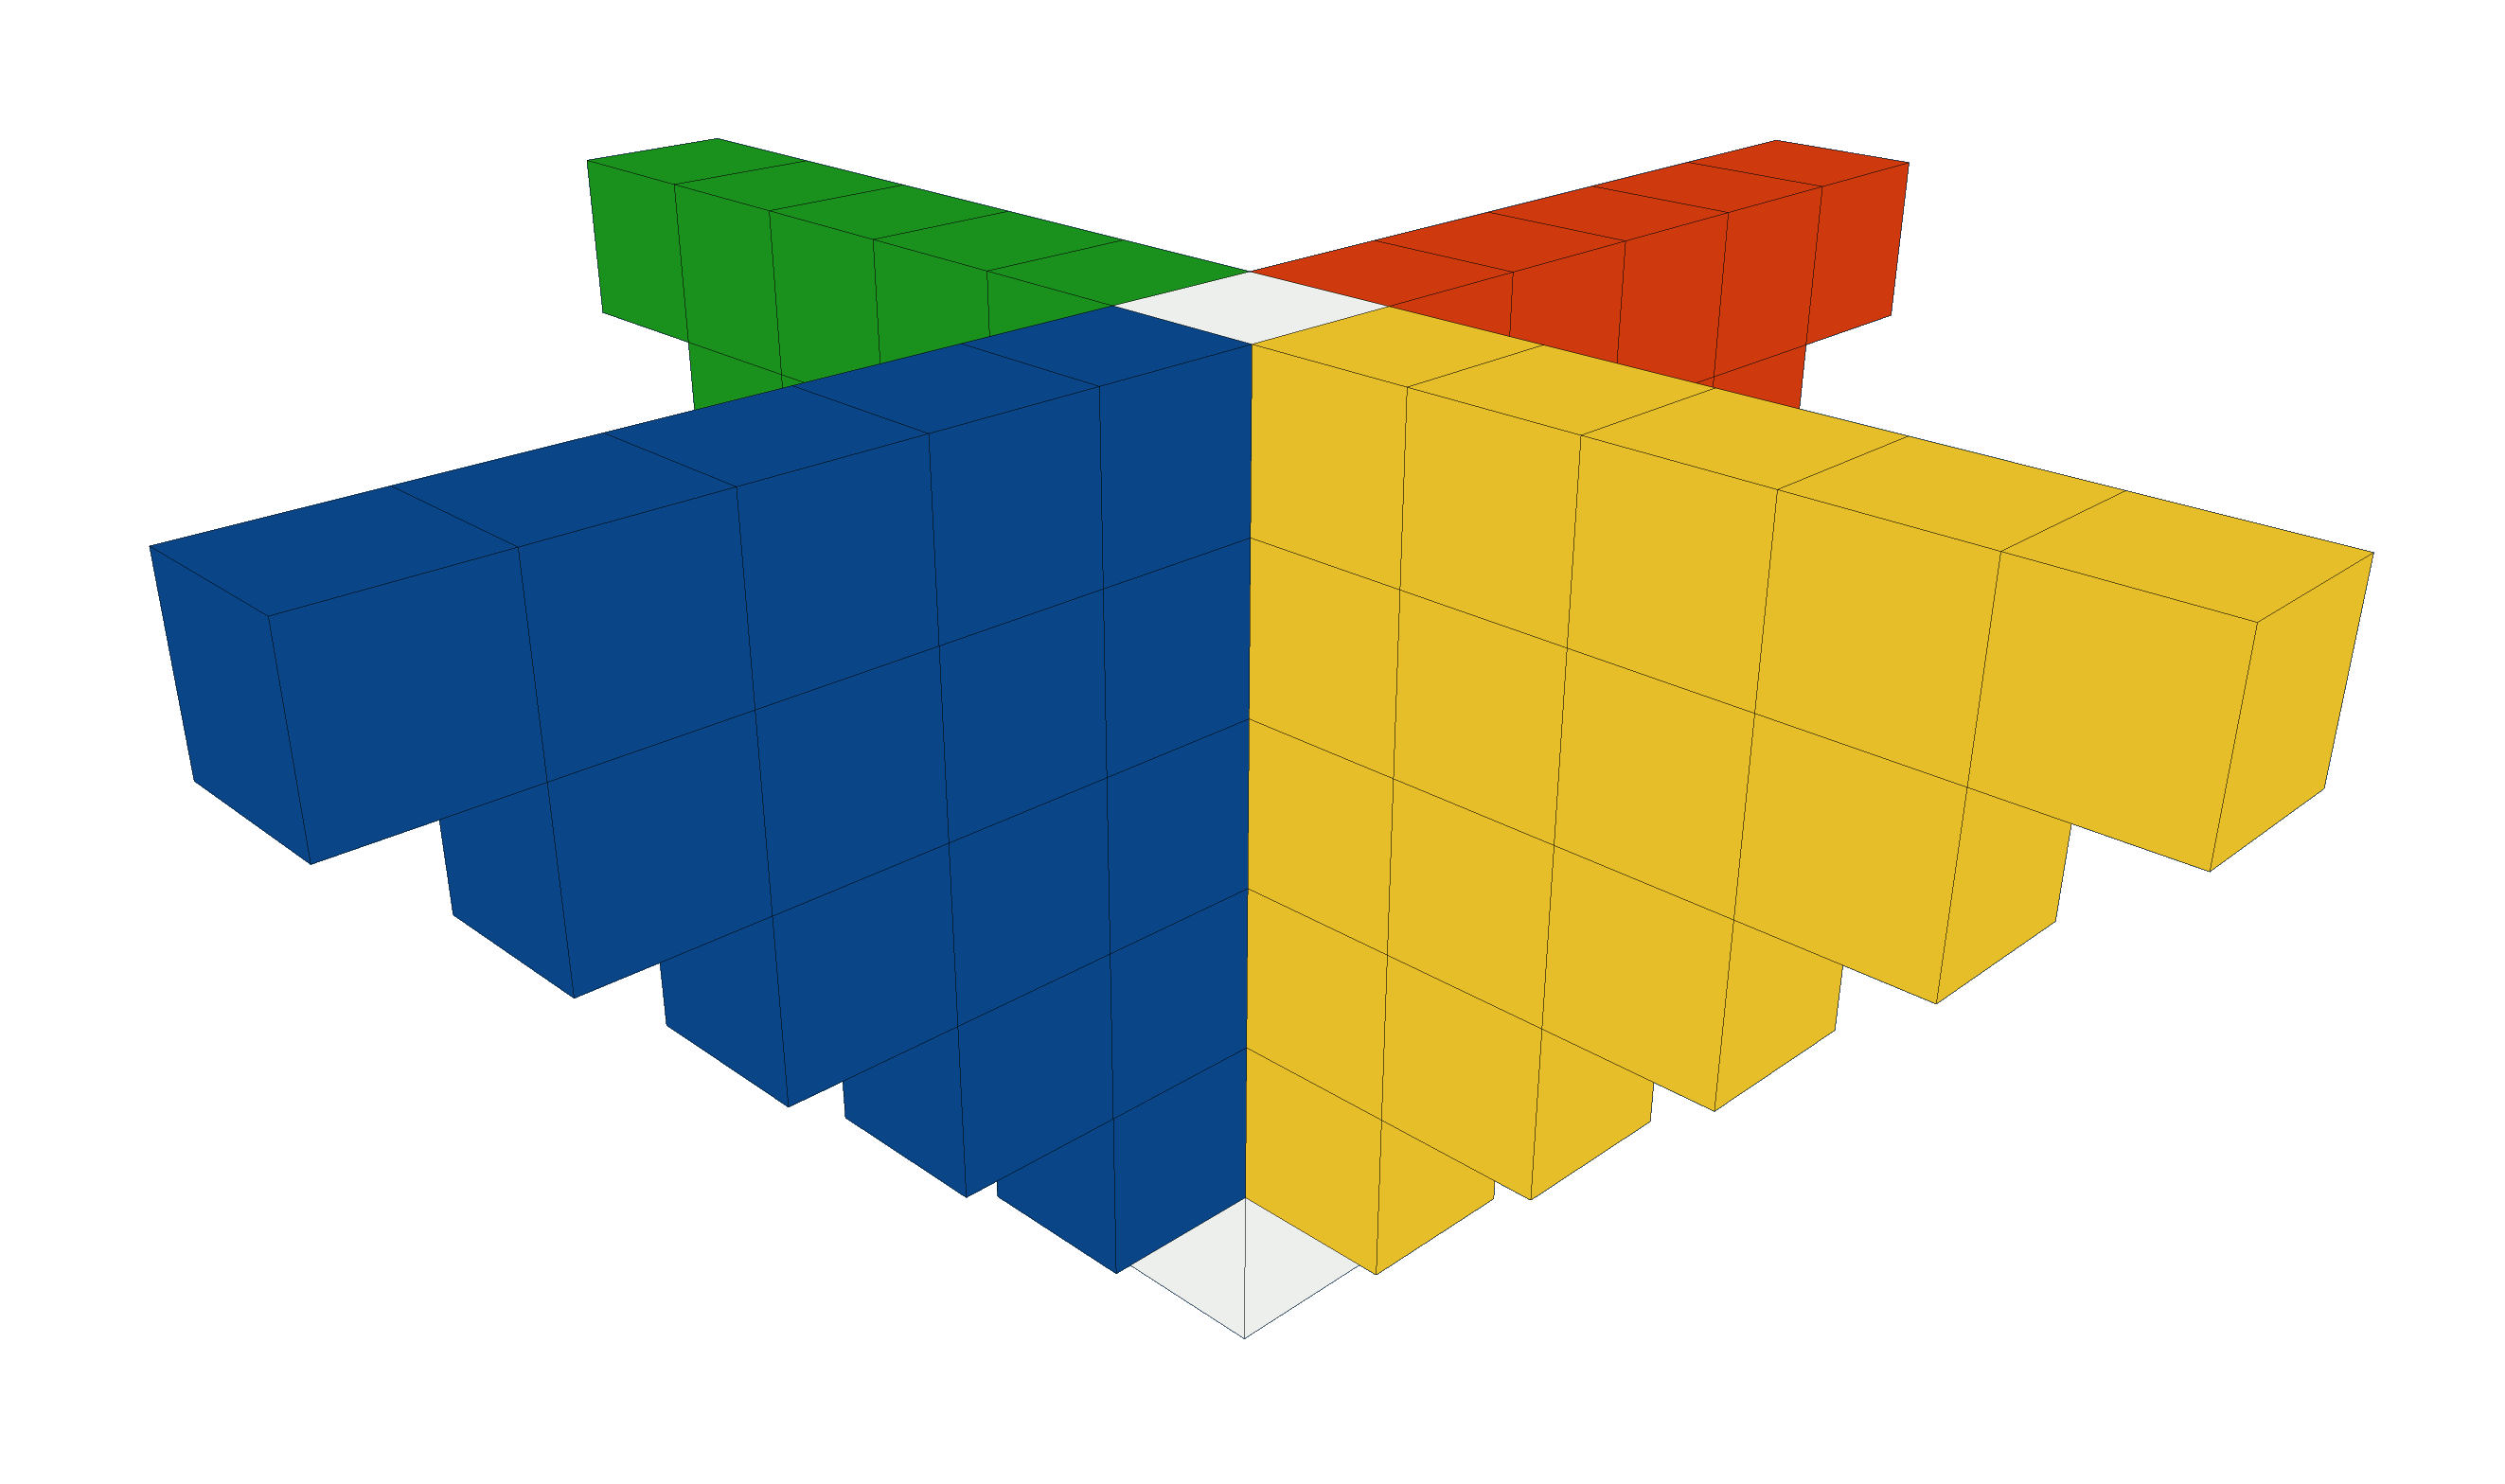
\includegraphics[height=0.1\textwidth]{../figures/angle3.png}\hspace{-3pt}
  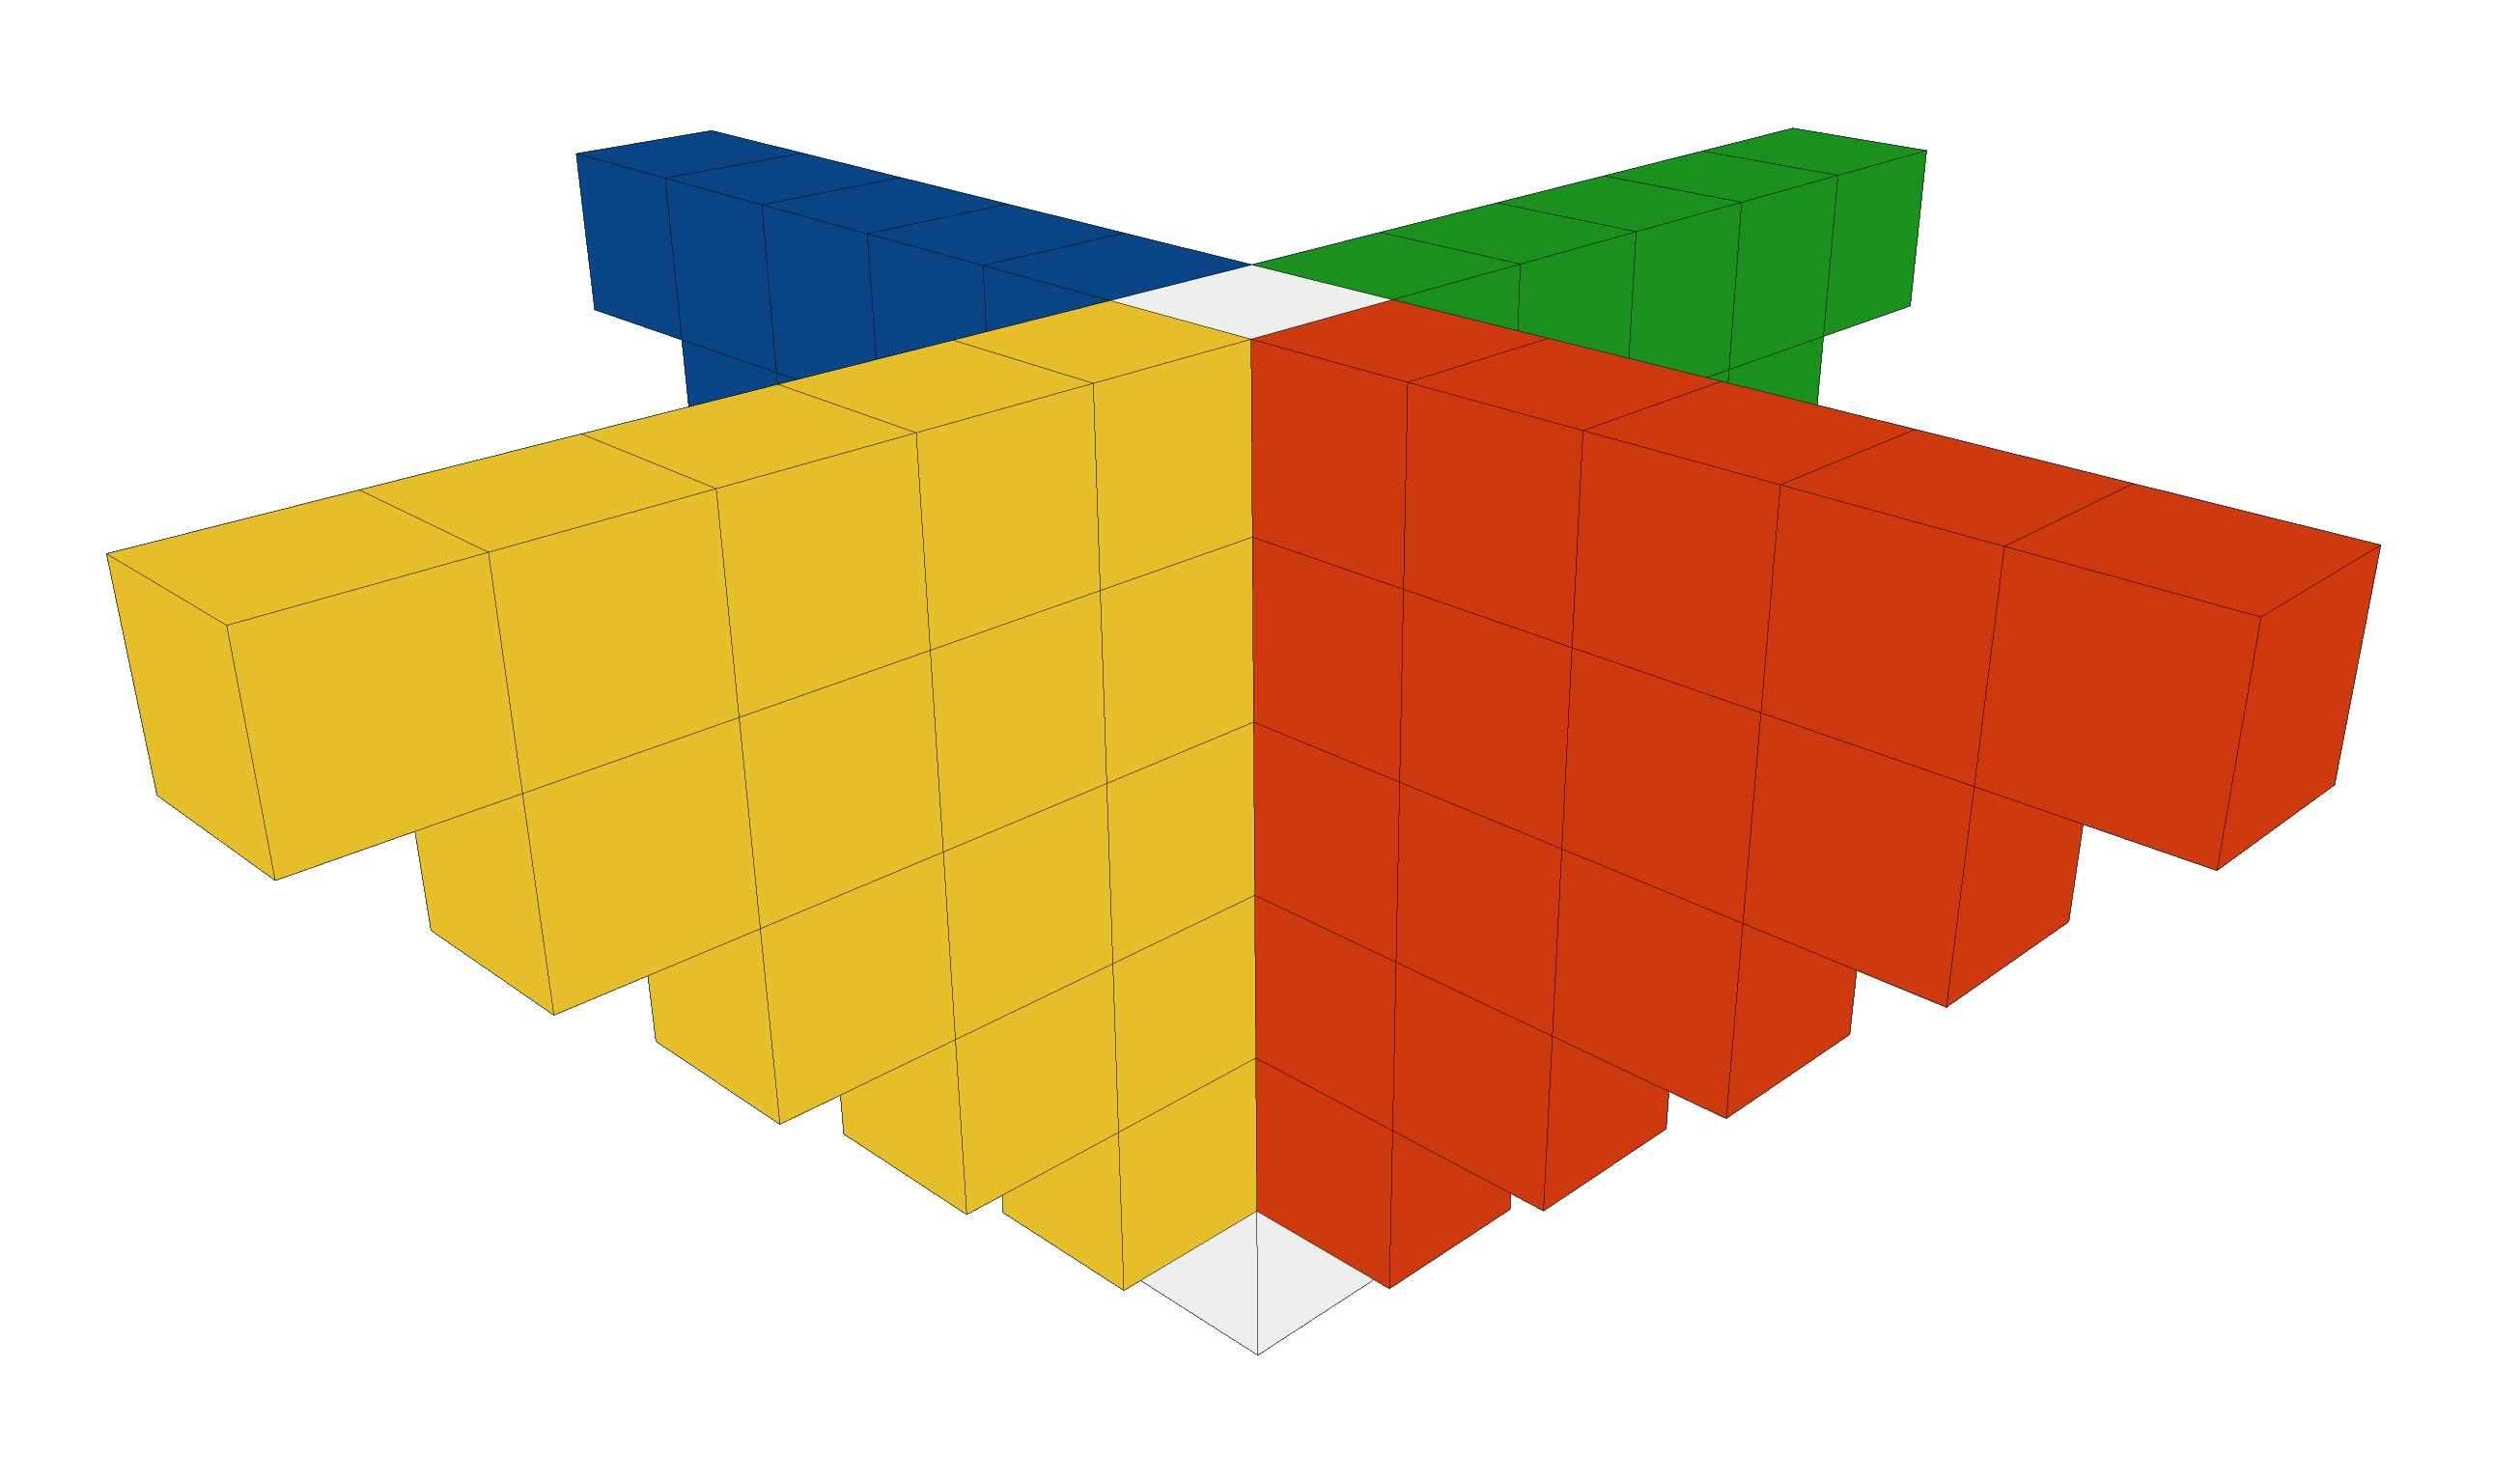
\includegraphics[height=0.1\textwidth]{../figures/angle4.png}
    \caption{Orientations of a $\bigcap_{i = 1}^4 \mathcal{L}(\mathcal{G}_i) \cap \Sigma ^6$ configuration. As $c \rightarrow \infty$, this shape approximates a circular cone whose symmetric axis joins $\sigma_i$ with orthonormal unit productions $w_i \rightarrow t_\cap$, and $S_i \in \Lambda^*_{\sigma}?$ represented by the outermost bitvector inhabitants. Equations of this form are equiexpressive with the family of CSLs realizable by finite CFL intersection.}
\end{figure}

It is a well-known fact in formal language theory that CFLs are closed under union, composition, substitution and intersection with regular languages, and the intersection between two CFLs is decidable. However CFLs are not closed under intersection, which requires a more general formalism. Following Okhotin~\cite{okhotin2001conjunctive}, we define higher-order grammar combinators $\cup, \cap: \mathcal{G}^*\times\mathcal{G}^*\rightarrow\mathcal{G}^*$ where $\mathcal{G}^*$ is a conjunctive grammar, which are basically finite collections of CFGs. Unlike parser combinators which are susceptible to ambiguity errors, our grammar combinators return parse forests in case of syntactic ambiguity, and do not suffer from the same shortcomings.

Given two CFLs $\mathcal{L}_\mathcal{G}, \mathcal{L}_{\mathcal{G}'}$, we can compute the intersection $\mathcal{L}_\mathcal{G}\cap\mathcal{L}_{\mathcal{G}'}\cap\Sigma^d$ by encoding $(\mathbf{M}_\mathcal{G}^*\sigma) = (\mathbf{M}_{\mathcal{G}'}^*\sigma)$. This allows us to build a DSL of grammar combinators to constrain the solution space.

For example, we can solve $\Sigma^d \cap \overline{\mathcal{L}_\mathcal{G}}$ by enumerating $\{\beta\sigma'\gamma \mid \sigma' \in \Sigma^d, \beta = \gamma = \_^k\}$, overapproximating the prefix and suffix (padding left and right), and checking for UNSAT to underapproximate \textit{impossible substrings}, strings which cannot appear in any $\{\sigma \in \mathcal{L}_\mathcal{G}\}$. Precomputing impossible substrings for a given grammar allows us to quickly eliminate inadmissible repairs and localize syntax errors in candidate strings.

Using the technique from Sec.~\ref{sec:levenshtein}, we can also compute language edit distance, the minimum number of Levenshtein edits required to fix a syntactically invalid string. Language intersection is significantly faster than approximating the gradient via sampling.

We can also build a set of grammars of increasing granularity, like a lattice structure. Basically, we can build up a lattice (in the order theoretic sense), consisting of grammars of increasing granularity. All programming languages require balanced parentheses, but some have additional constraints. So we can combine grammars, count and do bounded linear integer arithmetic.

\pagebreak\section{Error Recovery}\label{sec:error}

The matrix $\mathcal{M}^*$ encodes a superposition of all admissible binary trees of a fixed breadth. Consider the string \texttt{\_ ... \_}, which might generate various parse trees:

\begin{figure}[H]
  \resizebox{0.99\textwidth}{!}{
    \[
      \mathbf{M}^* = \begin{pNiceArray}{ccccccc}[margin, extra-margin=2pt,colortbl-like, xdots/line-style=loosely dotted]
         \tikzmark{a} & \tikzmark{k}  & \tikzmark{b} & \tikzmark{m} & \tikzmark{c} & \tikzmark{q} & \tikzmark{d} \\
                 \vno & \tikzmark{l}  &              & \tikzmark{n} &              & \tikzmark{r} & \tikzmark{w} \\
                 \vdd & \ddd          & \tikzmark{e} & \tikzmark{o} & \tikzmark{f} & \tikzmark{s} & \tikzmark{g} \\
                      &               &              & \tikzmark{p} &              & \tikzmark{t} & \tikzmark{x} \\
                      &               &              &              & \tikzmark{h} & \tikzmark{u} & \tikzmark{i} \\
                      &               &              &              &              & \tikzmark{v} &              \\
                 \vno & \cdd          &              &              &              & \vno         & \tikzmark{j}
      \end{pNiceArray}
      \begin{tikzpicture}[overlay, remember picture, blubr/.style={-,blue}, redbr/.style={-,red}, grnbr/.style={-,green}]
        \draw [grnbr] ({pic cs:l}) to ({pic cs:r});
        \draw [grnbr] ({pic cs:v}) to ({pic cs:r});
        \draw [grnbr] ({pic cs:r}) to ({pic cs:w});
        \draw [blubr] ({pic cs:a}) to ({pic cs:b});
        \draw [blubr] ({pic cs:e}) to ({pic cs:b});
        \draw [blubr] ({pic cs:h}) to ({pic cs:c});
        \draw [blubr] ({pic cs:b}) to ({pic cs:c});
        \draw [blubr] ({pic cs:c}) to ({pic cs:d});
        \draw [redbr] ({pic cs:h}) to ({pic cs:i});
        \draw [redbr] ({pic cs:j}) to ({pic cs:i});
        \draw [redbr] ({pic cs:e}) to ({pic cs:g});
        \draw [redbr] ({pic cs:i}) to ({pic cs:g});
        \draw [redbr] ({pic cs:g}) to ({pic cs:d});
      \end{tikzpicture}\Rightarrow
      \left\{\begin{pNiceArray}{ccccccc}[margin, extra-margin=2pt,colortbl-like, xdots/line-style=loosely dotted]
        \tikzmark{a1} & \tikzmark{k1}  & \tikzmark{b1} & \tikzmark{m1} & \tikzmark{c1} & \tikzmark{q1} & \tikzmark{d1} \\
        \vno          & \tikzmark{l1}  &               & \tikzmark{n1} &               & \tikzmark{r1} & \tikzmark{w1} \\
        \vdd          & \ddd           & \tikzmark{e1} & \tikzmark{o1} & \tikzmark{f1} & \tikzmark{s1} & \tikzmark{g1} \\
                      &                &               & \tikzmark{p1} &               & \tikzmark{t1} & \tikzmark{x1} \\
                      &                &               &               & \tikzmark{h1} & \tikzmark{u1} & \tikzmark{i1} \\
                      &                &               &               &               & \tikzmark{v1} &              \\
        \vno          & \cdd           &               &               &               & \vno          & \tikzmark{j1}
      \end{pNiceArray}
      \begin{tikzpicture}[overlay, remember picture, redbr/.style={-,red}]
        \draw [redbr] ({pic cs:a1}) to ({pic cs:d1});
        \draw [redbr] ({pic cs:h1}) to ({pic cs:i1});
        \draw [redbr] ({pic cs:j1}) to ({pic cs:i1});
        \draw [redbr] ({pic cs:e1}) to ({pic cs:g1});
        \draw [redbr] ({pic cs:i1}) to ({pic cs:g1});
        \draw [redbr] ({pic cs:g1}) to ({pic cs:d1});
      \end{tikzpicture}_{\textstyle,}
      \begin{pNiceArray}{ccccccc}[margin, extra-margin=2pt,colortbl-like, xdots/line-style=loosely dotted]
        \tikzmark{a2} & \tikzmark{k2}  & \tikzmark{b2} & \tikzmark{m2} & \tikzmark{c2} & \tikzmark{q2} & \tikzmark{d2} \\
        \vno          & \tikzmark{l2}  &               & \tikzmark{n2} &               & \tikzmark{r2} & \tikzmark{w2} \\
        \vdd          & \ddd           & \tikzmark{e2} & \tikzmark{o2} & \tikzmark{f2} & \tikzmark{s2} & \tikzmark{g2} \\
                      &                &               & \tikzmark{p2} &               & \tikzmark{t2} & \tikzmark{x2} \\
                      &                &               &               & \tikzmark{h2} & \tikzmark{u2} & \tikzmark{i2} \\
                      &                &               &               &               & \tikzmark{v2} &              \\
        \vno          & \cdd           &               &               &               & \vno          & \tikzmark{j2}
      \end{pNiceArray}
      \begin{tikzpicture}[overlay, remember picture, blubr/.style={-,blue}]
        \draw [blubr] ({pic cs:a2}) to ({pic cs:b2});
        \draw [blubr] ({pic cs:e2}) to ({pic cs:b2});
        \draw [blubr] ({pic cs:h2}) to ({pic cs:c2});
        \draw [blubr] ({pic cs:b2}) to ({pic cs:c2});
        \draw [blubr] ({pic cs:c2}) to ({pic cs:d2});
        \draw [blubr] ({pic cs:j2}) to ({pic cs:d2});
      \end{tikzpicture}_{\textstyle,}
      \begin{pNiceArray}{ccccccc}[margin, extra-margin=2pt,colortbl-like, xdots/line-style=loosely dotted]
        \tikzmark{a3} & \tikzmark{k3}  & \tikzmark{b3} & \tikzmark{m3} & \tikzmark{c3} & \tikzmark{q3} & \tikzmark{d3} \\
        \vno          & \tikzmark{l3}  &               & \tikzmark{n3} &               & \tikzmark{r3} & \tikzmark{w3} \\
        \vdd          & \ddd           & \tikzmark{e3} & \tikzmark{o3} & \tikzmark{f3} & \tikzmark{s3} & \tikzmark{g3} \\
                      &                &               & \tikzmark{p3} &               & \tikzmark{t3} & \tikzmark{x3} \\
                      &                &               &               & \tikzmark{h3} & \tikzmark{u3} & \tikzmark{i3} \\
                      &                &               &               &               & \tikzmark{v3} &              \\
        \vno          & \cdd           &               &               &               & \vno          & \tikzmark{j3}
      \end{pNiceArray}
      \begin{tikzpicture}[overlay, remember picture, grnbr/.style={-,green}]
        \draw [grnbr] ({pic cs:l3}) to ({pic cs:r3});
        \draw [grnbr] ({pic cs:n3}) to ({pic cs:p3});
        \draw [grnbr] ({pic cs:v3}) to ({pic cs:r3});
        \draw [grnbr] ({pic cs:r3}) to ({pic cs:w3});
        \draw [grnbr] ({pic cs:j3}) to ({pic cs:d3});
        \draw [grnbr] ({pic cs:a3}) to ({pic cs:d3});
      \end{tikzpicture}\ldots\right\}
    \]
  }
\end{figure}

\noindent Not only is Tidyparse capable of suggesting repairs to invalid strings, it can also return partial trees for those same strings, which is often helpful for debugging purposes. Unlike LL- and LR-style parsers which require special rules for error recovery, Tidyparse can simply analyze the structure of $M^*$ to recover parse branches. If $S \notin  \Lambda^*_\sigma$, the upper triangular entries of $M^*$ will take the form of a jagged-shaped ridge whose peaks signify the roots of maximally-parsable substrings $\hat{\sigma}_{i, j}$.

\begin{figure}[H]
  \hspace{-0.5cm}\begin{minipage}[l]{6cm}
      \[
        \begin{NiceMatrix}
          \leftarrow & \nse & \nsi & \nfi & \nfo & \nth & \ntw & \non & \leftarrow & \ppp \\
                     &      & \ddd & \ddd & \ddd & \ddd & \ddd & \ddd & \ddd & \ppp \\
      \sigma_1^\shri & \cdd &      & A    &      &      &      &      &      & \ppp \\
                \vno & \ddd &  T_A & \vdd &      &      &      &      &      & \ppp \\
                \vdd & \ddd &      & \pcd & \cdd &      & B    &      &      & \ppp \\
                     &      &      &      &      & T_B  & \vdd &      &      & \ppp \\
                     &      &      &      &      &      & \pcd & \cdd &      & C    \\
                     &      &      &      &      &      &      &      & T_C  & \vdd \\
                     &      &      &      &      &      &      &      &      & \\
                     &      &      &      &      &      &      &      &      & \\
                     &      &      &      &      &      &      &      &      & \\
                     &      &      &      &      &      &      &      & \ppp & \sigma_n^\shup \\
                \vno & \cdd &      &      &      &      &      &      & \vno &
        \end{NiceMatrix}
    \]
  \end{minipage}
  \hspace{1cm}
  \begin{minipage}[l]{6cm}
      \begin{halftidyinput}
      (*@\err{\texttt{⊤ and ⊤ ! and ⊥ xor ⊤ ! ⊤ and ⊥}}\caret{ }@*)
      \end{halftidyinput}

      \begin{verbatim}
    Recovered 3 parseable leaves:
      \end{verbatim}
      \noindent\hspace{0.64cm}\emoji{herb}\hspace{1.70cm}\emoji{herb}\hspace{1.98cm}\emoji{herb}\vspace{-5pt}
      \begin{verbatim}
    └── ! [3]   └── and [4]   └── xor [6]
      \end{verbatim}

      \begin{verbatim}
    Recovered 2 parseable branches:
      \end{verbatim}
    \hspace{0.64cm}\emoji{herb}\hspace{2.51cm}\emoji{herb}\vspace{-5pt}
      \begin{verbatim}
    └── S [0..2]     └── S [8..11]
        ├── ⊤ [0]        ├── S [8..9]
        ├── and [1]      │   ├── ! [8]
        └── ⊤ [2]        │   └── ⊤ [9]
                         ├── and [10]
                         └── ⊥ [11]
      \end{verbatim}
    \end{minipage}
  \caption{Peaks along the UT matrix ridge correspond to maximally parseable substrings. By recursing over upper diagonals of decreasing elevation and discarding all subtrees that fall under the shadow of another's canopy, we can recover the partial subtrees. The example depicted above contains three such branches, rooted at nonterminals $C, B, A$.}\label{fig:peaks}
\end{figure}

\noindent These branches are located on peaks of the upper triangular (UT) matrix ridge. As depicted in Fig.~\ref{fig:peaks}, we traverse the peaks by decreasing elevation to collect partial AST branches and display the highest nonoverlapping branches, in this case $T_C$ and $T_A$ to the user, to help them diagnose the parsing error and manually repair it.

\pagebreak\section{Nonterminal Stubs}

Tidyparse augments CFGs with two additional rules, which are desugared into a vanilla CFG before parsing. The first rule, $\alpha\textsc{-sub}$, allows the user to define a nonterminal parameterized by $\alpha$, a non-recursive nonterminal in the same the CFG representing some finite type and its inhabitants. $\alpha\textsc{-sub}$ replaces all productions containing $\langle\alpha\rangle$ with the terminals in their transitive closure, $\alpha \rightarrow^* \beta$. The second rule, $\alpha\textsc{-int}$, introduces homonymous terminals for each user-defined nonterminal.

\begin{figure}[H]
\begin{prooftree}
\AxiomC{$\mathcal{G} \vdash (w\langle\alpha\rangle \rightarrow x z) \in P$}
\AxiomC{$\alpha^* : \{\beta \mid (\alpha \rightarrow^* \beta) \in P\}$}
\RightLabel{$\alpha\textsc{-sub}$}
\BinaryInfC{$\mathcal{G} \vdash \forall \beta \in \alpha^*.(w\langle\alpha\rangle \rightarrow x z)[\beta/\alpha] \in P'$}
\DisplayProof
\hskip 1.5em
\AxiomC{$\mathcal{G} \vdash v \in V$}
\RightLabel{$\langle\cdot\rangle\textsc{-int}$}
\UnaryInfC{$\mathcal{G} \vdash (v \rightarrow \langle v\rangle) \in P$}
\end{prooftree}
\end{figure}

\noindent Some dependently typed programming languages can do parsing in the type checker -- our parser can also perform some form of type checking. Tidyparse automatically expands typed expressions into ordinary nonterminals using the $\alpha\textsc{-sub}$ rule, for example when parsing an expression of the form $x + y$, the grammar will recognize \texttt{true + false} and \texttt{1 + 2}, but not \texttt{1 + true}.

\begin{tcolorbox}[left skip=0.7cm,
top=0.1cm,
middle=0mm,
boxsep=0mm,
underlay unbroken and first={%
\path[draw=none] (interior.north west) rectangle node[white]{
\includegraphics[width=4mm]{../figures/tidyparse_logo.png}} ([xshift=-10mm,yshift=-9mm]interior.north west);
}]
\begin{lstlisting} [language=tidy, basicstyle=\ttfamily\small, escapeinside={(*@}{@*)}]
E<X> -> E<X> + E<X> | E<X> * E<X> | ( E<X> )
X -> Int | Bool
\end{lstlisting}
\tcblower
\begin{lstlisting} [language=tidy, basicstyle=\ttfamily\small, escapeinside={(*@}{@*)}]
E<Int> -> E<Int> + E<Int> | E<Int> * E<Int>
E<Bool> -> E<Bool> + E<Bool> | E<Bool> * E<Bool>
\end{lstlisting}
\end{tcolorbox}

When completing a bounded-width string, one finds it is often convenient to admit nonterminal stubs, representing unexpanded subexpressions. To enable this functionality, we introduce a synthetic production for each $v \in V$ using the $\langle\cdot\rangle\textsc{-int}$ rule. Users can interactively build up a complex expression by placing the caret over a stub, then pressing \keys{\ctrl + \SPACE}:

\begin{tcolorbox}[left skip=0.7cm,
top=0.1cm,
middle=0mm,
boxsep=0mm,
underlay unbroken and first={%
\path[draw=none] (interior.north west) rectangle node[white]{
\includegraphics[width=4mm]{../figures/tidyparse_logo.png}} ([xshift=-10mm,yshift=-9mm]interior.north west);
}]
\begin{lstlisting} [language=tidy, basicstyle=\ttfamily\small, escapeinside={(*@}{@*)}]
false or ! true or <(*@\caret{S}@*)> and <S> or <S>
\end{lstlisting}
\tcblower
\begin{lstlisting} [language=tidy, basicstyle=\ttfamily\small, escapeinside={(*@}{@*)}]
1.) false or ! true or (*@\hlorange{true}@*) and <S> or <S>
2.) false or ! true or (*@\hlorange{false}@*) and <S> or <S>
3.) false or ! true or (*@\hlorange{!}@*) (*@\hlorange{<S>}@*) and <S> or <S>
4.) false or ! true or (*@\hlorange{<S>}@*) (*@\hlorange{and}@*) (*@\hlorange{<S>}@*) and <S> or <S>
5.) false or ! true or (*@\hlorange{<S>}@*) (*@\hlorange{or}@*) (*@\hlorange{<S>}@*) and <S> or <S>
...
\end{lstlisting}
\end{tcolorbox}

\noindent This functionality can also be useful inside a completion, which might be expanded as follows:

\begin{tcolorbox}[left skip=0.7cm,
top=0.1cm,
middle=0mm,
boxsep=0mm,
underlay unbroken and first={%
\path[draw=none] (interior.north west) rectangle node[white]{
\includegraphics[width=4mm]{../figures/tidyparse_logo.png}} ([xshift=-10mm,yshift=-9mm]interior.north west);
}]
\begin{lstlisting} [language=tidy, basicstyle=\ttfamily\small, escapeinside={(*@}{@*)}]
if <Vexp> _ _ _ _ _(*@\caret{ }@*)
\end{lstlisting}
\tcblower
\begin{lstlisting} [language=tidy, basicstyle=\ttfamily\small, escapeinside={(*@}{@*)}]
1.) if (*@\hlorange{map}@*) X then <Vexp> else <Vexp>
2.) if (*@\hlorange{uncurry}@*) X then <Vexp> else <Vexp>
3.) if (*@\hlorange{foldright}@*) X then <Vexp> else <Vexp>
...
\end{lstlisting}
\end{tcolorbox}

\pagebreak\section{Practical Example}

Tidyparse requires a grammar, which can either be provided by the user or ingested from a BNF specification. The following grammar represents a slightly more realistic programming language:

\begin{tcolorbox}[left skip=0.7cm,
top=0.1cm,
middle=0mm,
boxsep=0mm,
underlay unbroken and first={%
\path[draw=none] (interior.north west) rectangle node[white]{
\includegraphics[width=4mm]{../figures/tidyparse_logo.png}} ([xshift=-10mm,yshift=-9mm]interior.north west);
}]
\begin{lstlisting} [language=tidy, basicstyle=\ttfamily\small, escapeinside={(*@}{@*)}]
S -> A | V | ( X , X ) | X X | ( X )
A -> Fun | F | L | L in X
Fun -> fun V (*@`@*)->(*@`@*) X
F -> if X then X else X
L -> let V = X | let rec V = X
V -> Vexp | ( Vexp ) | Vexp Vexp
Vexp -> VarName | FunName | Vexp VO Vexp | ( VarName , VarName ) | Vexp Vexp
VarName -> a | b | c | d | e | ... | z
FunName -> foldright | map | filter | curry | uncurry
VO ->  + | - | * | / | > | = | < | (*@`@*)||(*@`@*) | &&
---
let curry f = ( fun x y -> f ( _ _ _(*@\caret{ }@*)) )
\end{lstlisting}
\tcblower
\begin{lstlisting} [language=tidy, basicstyle=\ttfamily\small, escapeinside={(*@}{@*)}]
let curry f = ( fun x y -> f ( (*@\hlorange{<X>}@*) ) )
let curry f = ( fun x y -> f ( (*@\hlorange{<FunName>}@*) ) )
let curry f = ( fun x y -> f ( (*@\hlorange{curry}@*) (*@\hlorange{<X>}@*) ) )
...
\end{lstlisting}
\end{tcolorbox}

\noindent We can also handle error correction and completion in the untyped \lambda-calculus, as shown below:

\begin{tcolorbox}[left skip=0.7cm,
top=0.1cm,
middle=0mm,
boxsep=0mm,
underlay unbroken and first={%
\path[draw=none] (interior.north west) rectangle node[white]{
\includegraphics[width=4mm]{../figures/tidyparse_logo.png}} ([xshift=-10mm,yshift=-9mm]interior.north west);
}]
\begin{lstlisting} [language=tidy, basicstyle=\ttfamily\small, escapeinside={(*@}{@*)}]
sxp -> λ var . sxp | sxp sxp | var | ( sxp ) | const
const -> 1 | 2 | 3 | 4 | 5 | 6
var -> a | b | c | f | x | y | z
---
( λ f . ( λ x . f ( x x ) ) ( λ x . f ( x x ) (*@\caret{ }@*)
\end{lstlisting}
\tcblower
\begin{lstlisting} [language=tidy, basicstyle=\ttfamily\small, escapeinside={(*@}{@*)}]
1.) ( λ f . ( λ x . f ( x x ) ) (*@\hlorange{)}@*) λ x . f ( x x )
2.) ( λ f . ( λ x . f ( x x ) ) (*@\hlorange{x}@*) (*@\hlgreen{)}@*) λ x . f ( x x )
3.) ( λ f . ( λ x . f ( x x ) ) ( λ x . f ( x(*@\hlred{ }@*)) (*@\hlgreen{)}@*) (*@\hlgreen{)}@*)
...
\end{lstlisting}
\end{tcolorbox}

\pagebreak\subsection{Grammar Assistance}

Tidyparse uses a CFG to parse the CFG, so it can provide assistance while the user is designing the CFG. For example, if the CFG does not parse, it will suggest possible fixes. In the future, we intend to use this functionality to perform example-based codesign and grammar induction.

\begin{tcolorbox}[left skip=0.7cm,
top=0.1cm,
middle=0mm,
boxsep=0mm,
underlay unbroken and first={%
\path[draw=none] (interior.north west) rectangle node[white]{
\includegraphics[width=4mm]{../figures/tidyparse_logo.png}} ([xshift=-10mm,yshift=-9mm]interior.north west);
}]
\begin{lstlisting} [language=tidy, basicstyle=\ttfamily\small, escapeinside={(*@}{@*)}]
B -> true | false | (*@\caret{ }@*)
\end{lstlisting}
\tcblower
\begin{lstlisting} [language=tidy, basicstyle=\ttfamily\small, escapeinside={(*@}{@*)}]
B -> true | false (*@\hlred{ }@*)
B -> true | false (*@\hlorange{<RHS>}@*)
B -> true | false | (*@\hlgreen{<RHS>}@*)
...
\end{lstlisting}
\end{tcolorbox}

\subsection{Interactive Nonterminal Expansion}

Users can interactively build up a complex expression by placing the caret over a stub they wish to expand, then pressing \keys{\ctrl + \SPACE}:

\begin{tcolorbox}[left skip=0.7cm,
top=0.1cm,
middle=0mm,
boxsep=0mm,
underlay unbroken and first={%
\path[draw=none] (interior.north west) rectangle node[white]{
\includegraphics[width=4mm]{../figures/tidyparse_logo.png}} ([xshift=-10mm,yshift=-9mm]interior.north west);
}]
\begin{lstlisting} [language=tidy, basicstyle=\ttfamily\small, escapeinside={(*@}{@*)}]
if <(*@\caret{V}@*)exp> X then <Vexp> else <Vexp>
\end{lstlisting}
\tcblower
\begin{lstlisting} [language=tidy, basicstyle=\ttfamily\small, escapeinside={(*@}{@*)}]
if (*@\hlorange{map}@*) X then <Vexp> else <Vexp>
if (*@\hlorange{uncurry}@*) X then <Vexp> else <Vexp>
if (*@\hlorange{foldright}@*) X then <Vexp> else <Vexp>
...
\end{lstlisting}
\end{tcolorbox}

\subsection{Conjunctive Grammars}

Many natural and programming languages exhibit context-sensitivity, such as Python indentation. Unlike traditional parser-generators, Tidyparse can encode CFL intersection, allowing it to detect and correct errors in a more expressive family of languages than would ordinarily be possible using CFGs alone. For example, consider the grammar from Sec.~\ref{sec:lclreach}:

\begin{tcolorbox}[left skip=0.7cm,
top=0.1cm,
middle=0mm,
boxsep=0mm,
underlay unbroken and first={%
\path[draw=none] (interior.north west) rectangle node[white]{
\includegraphics[width=4mm]{../figures/tidyparse_logo.png}} ([xshift=-10mm,yshift=-9mm]interior.north west);
}]
\begin{lstlisting} [language=tidy, basicstyle=\ttfamily\small, escapeinside={(*@}{@*)}]
S -> L R    L -> a b | a L b    R -> c | c R    &&&
S -> L R    R -> b c | b R c    L -> a | a L
---
_ _ _ _ _ _ _ _ _ _ _ _ _ _ _ _ _ _ _ _(*@\caret{ }@*)
\end{lstlisting}
\tcblower
\begin{lstlisting} [language=tidy, basicstyle=\ttfamily\small, escapeinside={(*@}{@*)}]
1.) a b c
2.) a a b b c c
3.) a a a b b b c c c
4.) a a a a b b b b c c c c
...
\end{lstlisting}
\end{tcolorbox}

\noindent Tidyparse uses the notation \texttt{G1} {\color{blue}\texttt{\&\&\&}} \texttt{G2} and \texttt{G1} {\color{blue}\texttt{|||}} \texttt{G2} to signify $\mathcal{L}_{\mathcal{G}_1}\cap\mathcal{L}_{\mathcal{G}_2}$ and $\mathcal{L}_{\mathcal{G}_1}\cup\mathcal{L}_{\mathcal{G}_2}$ respectively, i.e., the intersection or union of two or more grammars' languages. {Composition}, complementation and other operations on finite languages are also possible, although undocumented at present.

%There are some more examples too.
%
%The line between parsing and computation is blurry.

\section{Related Work}

The literature on parsers is vast and deep, covering far more ground than we could possibly hope to survey. We take inspiration from their findings, but restrict ourselves to a dozen most closely related papers, in four major research areas: (1) formal language theory, (2) constraint satisfaction (3) program synthesis, and (4) error correction. We survey each of these areas in turn.

It was Noam Chomsky himself who first developed the algebraic theory of \textit{context-free grammars} (CFGs) in 1959~\cite{chomsky1959algebraic}, and since then, CFGs have been the subject of extensive research in formal language theory and program analysis. In particular, we take inspiration from Leslie Valiant~\cite{valiant1975general} who first discovered the connection to matrix multiplication in 1975 and Alexander Okhotin~\cite{okhotin2001conjunctive} who later introduced the idea of \textit{conjunctive grammars} in 2001. More recently, Azimov \& Grigorev~\cite{azimov2018cfpq} and Qirun Zhang shed light into the practical applicability of these ideas and made the theory of CFG reachability more accessible to the general public. In our work, we show how to compile their ideas onto a SAT solver to fix syntax errors, which seems like a perfectly natural extension, but was heretofore previously never considered to the best of our knowledge.

There is related work on string constraint solving in the constraint programing literature, featuring solvers like CFGAnalyzer and HAMPI~\cite{kiezun2009hampi}, which consider bounded context free grammars and intersections thereof. Axelson et al. (2008)~\cite{axelsson2008analyzing} has some work on incremental SAT encoding but does not exploit the linear-algebraic structure of parsing nor provide real-time guarantees. Finally, Loris D'Antoni did some great work on \textit{symbolic automata}~\cite{dantoni2014minimization}, a generalization of finite automata which allow allow infinite alphabets and symbolic expressions over them. In none of the constraint programming literature we surveyed do any of the approaches employ matrix-based parsing, and therefor do not enjoy the optimality guarantees of Valiant's parser. Our solver can handle CFGs and conjunctive grammars with finite alphabets and does not require any special grammar encoding. The matrix encoding makes it particularly amenable to parallelization.

In program synthesis, we direct our attention to the problem of \textit{incremental synthesis} or \textit{error correction}, which is the problem of synthesizing programs incrementally while the user is typing. Modern research on error correction can be traced back to the early days of coding theory, when researchers designed \textit{error-correcting codes} (ECCs) to denoise transmission errors induced by external interference, whether due to collision with a high-energy proton, manipulation by an adversary or some typographical mistake. In this context, \textit{code} can be any logical representation for communicating information between two parties (such as a human and a computer), and an ECC is a carefully-designed code which ensures that even if some portion of the message should be corrupted through accidental or intentional means, one can still recover the original message by solving a linear system of equations. In particular, we frame our work inside the context of errors arising from human factors in computer programming.

In programming, most such errors initially manifest as syntax errors, and though often cosmetic, manual repair can present a significant challenge for novice programmers. The ECC problem may be refined by introducing a language, $\mathcal{L} \subset \Sigma^*$ and considering admissible edits transforming an arbitrary string, $s \in \Sigma^*$ into a string, $s'\in\mathcal{L}$. Known as \textit{error-correcting parsing} (ECP), this problem was well-studied in the early parsing literature by Aho and Peterson~\cite{aho1972minimum}, but fell out of favor for many years, perhaps due to its perceived complexity. By considering only minimal-length edits, ECP can be reduced to the so-called \textit{language edit distance} (LED) problem, recently shown to be subcubic~\cite{bringmann2019truly}, suggesting its tractability. Previous LED results were primarily of a theoretical nature, but now, thanks to our contributions, we have finally realized a practical prototype.

In our work, we recast the problem of ECP as a special case of tensor completion with an logical semiring, and lay the foundation for a new approach to program repair grounded in formal language theory, unifying \textit{code completion}, \textit{error correction} and \textit{incremental parsing}. We provide exact and approximate algorithms for solving these problems in the real-world setting, and implement them in a real-time editor called Tidyparse, demonstrating their practical utility. Given a well-formed grammar, our tool can be used to complete unfinished code, parse incomplete code and repair broken fragments in arbitrary context-free and linear conjunctive languages.

\section{Latency Benchmark}\label{sec:latency}

In the following benchmarks, we measure the wall clock time required to synthesize solutions to length-50 strings sampled from various Dyck languages, where Dyck-n is the Dyck language containing n different types of balanced parentheses.

\begin{wholetidyinput}
Dyck-1 -> ( ) | ( Dyck-1 ) | Dyck-1 Dyck-1
Dyck-2 -> Dyck-1 | [ ] | ( Dyck-2 ) | [ Dyck-2 ] | Dyck-2 Dyck-2
Dyck-3 -> Dyck-2 | { } | ( Dyck-3 ) | [ Dyck-3 ] | { Dyck-3 } | Dyck-3 Dyck-3
\end{wholetidyinput}

\noindent In the first experiment, we sample a random valid string $\sigma \sim \Sigma^{50} \cap \mathcal{L}_{\text{Dyck-n}}$, then replace a fixed number of tokens with holes and measure the average time required to decode ten syntactically-admissible repairs across 100 trial runs.

\begin{figure}[H]
\hspace{-0.25cm}\begin{tikzpicture}[scale=0.8]
\begin{axis}[
width=8.3cm,
height=6cm,
title={\hspace{-1cm}\textbf{Latency with known locations}},
ybar,
bar width=6pt,
xlabel={Number of holes},
ylabel={ms to synthesize 10 repairs},
xtick=data,
axis x line*=bottom,
axis y line*=left,
ytick pos=left,
xticklabels from table={\loctimings}{holes},
ymajorgrids,
legend pos=north west,
legend columns=2,
error bars/y dir=both,
error bars/y explicit
]
\addplot table [x expr=\coordindex, y=d1, y error=d1err]{\loctimings};
\addplot table [x expr=\coordindex, y=d2, y error=d2err]{\loctimings};
\addplot table [x expr=\coordindex, y=d3, y error=d3err]{\loctimings};
\addplot table [x expr=\coordindex, y=d4, y error=d4err]{\loctimings};
\legend{Dyck-1, Dyck-2, Dyck-3, Dyck-4}
\end{axis}
\end{tikzpicture}
\begin{tikzpicture}[scale=0.8]
\begin{axis}[
width=8.3cm,
height=6cm,
title={\hspace{-1cm}\textbf{Latency with unknown locations}},
ybar,
bar width=20pt,
xlabel={Number of errors},
%ylabel={ms to synthesize 1 repair},
xtick=data,
axis x line*=bottom,
axis y line*=left,
enlarge x limits={abs=0.5},
ymode=log,
ytick pos=left,
xticklabels from table={\unloctimings}{errors},
ymajorgrids,
legend pos=north west,
error bars/y dir=both,
error bars/y explicit
]
\addplot table [x expr=\coordindex, y=d1]{\unloctimings};
\addplot table [x expr=\coordindex, y=d2]{\unloctimings};
\addplot table [x expr=\coordindex, y=d3]{\unloctimings};
\legend{Dyck-1, Dyck-2, Dyck-3}
\end{axis}
\end{tikzpicture}
\end{figure}

\noindent In the second experiment, we sample a random valid string as before, but delete p tokens at random and rather than provide the location(s), ask our model to solve for both the location(s) and repair by sampling uniformly from all n-token HCs, then measure the total time required to decode the first admissible repair. Note the logarithmic scale on the y-axis.

\pagebreak\section{Accuracy Benchmark}

In the following benchmark, we analyze bracketing errors in a dataset of Java and Python code snippets mined from open-source repositories on GitHub. For Java, we sample valid single-line statements with bracket nesting more than two levels deep, synthetically delete one bracket uniformly at random, repair using Tidyparse\footnote{Using the Dyck-n grammar augmented with \texttt{D1} {\color{blue}\texttt{->}} \texttt{w} {\color{blue}\texttt{|}} \texttt{D1}. Contiguous non-bracket tokens are substituted with a single placeholder token, \texttt{w}, and restored verbatim after bracket repair.}, then take the top-1 repair after $t$ seconds, and validate using ANTLR's Java 8 parser.

\begin{figure}[H]
\vspace{0.25cm}
%\adjustbox{scale=0.48,center}{%
\begin{tikzpicture}[scale=0.8]
\begin{axis}[
width=8.3cm,
height=6.6cm,
%    title={\hspace{-1cm}\textbf{Java Brackets}},
ybar,
bar width=10pt,
xlabel={$|\Sigma^*|$},
ylabel={Parser acceptance},
title={\textbf{Synthetic error correction accuracy}},
xtick=data,
axis x line*=bottom,
axis y line*=left,
enlarge x limits={abs=0.5},
ytick pos=left,
xticklabels from table={\syntheticerrors}{len},
ymajorgrids,
legend pos=north east,
legend columns=3,
error bars/y dir=both,
error bars/y explicit
]
\addplot table [x expr=\coordindex, y=10s]{\syntheticerrors};
\addplot table [x expr=\coordindex, y=30s]{\syntheticerrors};
\addplot table [x expr=\coordindex, y=60s]{\syntheticerrors};
\legend{10s, 30s, 60s}
\end{axis}
\end{tikzpicture}
\begin{tikzpicture}[scale=0.8]
\begin{axis}[
width=8.3cm,
height=6.6cm,
title={\textbf{Organic error correction accuracy}},
ybar,
bar width=10pt,
xlabel={$|\Sigma^*|$},
%ylabel={Parser acceptance},
xtick=data,
axis x line*=bottom,
axis y line*=left,
enlarge x limits={abs=0.5},
ytick pos=left,
xticklabels from table={\naturalerrors}{len},
ymajorgrids,
y tick label style={/pgf/number format/.cd,%
scaled y ticks = false,
set thousands separator={},
fixed},
legend pos=north east,
legend columns=3,
error bars/y dir=both,
error bars/y explicit
]
\addplot table [x expr=\coordindex, y=10s]{\naturalerrors};
\addplot table [x expr=\coordindex, y=30s]{\naturalerrors};
\addplot table [x expr=\coordindex, y=60s]{\naturalerrors};
\legend{10s, 30s, 60s}
\end{axis}
\end{tikzpicture}
\end{figure}

\noindent For Python, we sample invalid code fragments uniformly from the imbalanced bracket category of the Break-It-Fix-It (BIFI) dataset~\cite{yasunaga2021break}, a dataset of organic Python errors, repair using Tidyparse, take the top-1 repair after $t$ seconds, and validate repairs using Python's \texttt{ast.parse()} method.

%As expected, accuracy on organic errors in Python is lower.
%
%\subsection{Task Difficulty}
%
%\noindent\textbf{Level \textonehalf} - Incomplete code (all missing tokens at end)
%
%\noindent\textbf{Level 1} - Known number of errors at known locations
%
%\noindent\textbf{Level 2} - Known number of errors at unknown locations
%
%\noindent\textbf{Level 3} - Unknown number of errors at unknown locations
%
%\subsection{Repair Datasets}
%Synthetic - Synthetic errors in natural code snippets\\
%Natural - Natural errors and fixes mined from Git history
%\subsection{Evaluation Metrics}
%Syntactic validity - Only considers whether the repair parses\\
%Repair alignment - Measures string distance to true fix
%\subsection{Model configurations}
%Model configurations - LLM, ECP, ECP + LLM
%GraphCodeBERT
%RobertA
%Incoder
%CarperAI?

\pagebreak\section{Discussion}\label{sec:discussion}

While error correction with a few errors is tolerable, latency can vary depending on many factors including string length and grammar size. If errors are localized to the beginning or end of a string, then latency is typically below 500ms. We observe that errors are typically concentrated nearby historical edit locations, which can be retrieved from the IDE or version control.

Tidyparse in its current form has a number of technical shortcomings: firstly it does not incorporate any neural language modeling technology at present, an omission we hope to address in the near future. Training a language model to predict likely repair locations and rank admissible results could lead to lower overall latency and more natural repairs.

Secondly, our current method generates sketch templates using a na\"ive enumerative search, feeding them individually to the SAT solver, which has the tendency to duplicate prior work and introduces unnecessary thrashing. Considering recent extensions of Boolean matrix-based parsing to linear context-free rewriting systems (LCFRS)~\cite{cohen2016parsing}, it may be feasible to search through these edits within the SAT solver, leading to yet unrealized and possibly significant speedups.

Lastly and perhaps most significantly, Tidyparse does not incorporate any semantic constraints, so its repairs while syntactically admissible, are not guaranteed to be semantically valid. We note however, that it is possible to encode type-based semantic constraints into the solver and intend to explore this direction more fully in future work.

Not only is linear algebra over finite fields an expressive language for inference, but also an efficient framework for inference on languages themselves. We illustrate a few of its applications for parsing incomplete strings and repairing syntax errors in context- free and sensitive languages. In contrast with LL and LR-style parsers, our technique can recover partial forests from invalid strings by examining the structure of $M^*$ and handles arbitrary context-free langauges. In future work, we hope to extend our method to more natural grammars like PCFG and LCFRS.

We envision three primary use cases: (1) helping novice programmers become more quickly familiar with a new programming language (2) autocorrecting common typos among proficient but forgetful programmers and (3) as a prototyping tool for PL designers and educators. Featuring a grammar editor and built-in SAT solver, Tidyparse helps developers navigate the language design space, visualize syntax trees, debug parsing errors and quickly generate simple examples and counterexamples for testing. %Although the algorithm may seem esoteric at first glance, in our experience it is much more interpretable than classical parsers, which exhibit poor error-recovery and diagnostics.

\section{Conclusion}

Tidyparse accepts a CFG and a string to parse. If the string is valid, it returns the parse forest, otherwise, it returns a set of repairs, ordered by their Levenshtein edit distance to the invalid string. Our method compiles each CFG and candidate string onto a matrix dynamical system using an extended version of Valiant's construction and solves for its fixedpoints using an incremental SAT solver. This approach to parsing has many advantages, enabling us to repair syntax errors, correct typos and generate parse trees for incomplete strings. By allowing the string to contain holes, repairs can contain either concrete tokens or nonterminals, which can be manually expanded by the user or a neural-guided search procedure. From a theoretical standpoint, this technique is particularly amenable to neural program synthesis and repair, naturally integrating with the masked-language-modeling task (MLM) used by transformer-based neural language models.

From a practical standpoint, we have implemented our approach as an IDE plugin and demonstrated its viability as a tool for live programming. Tidyparse is capable of generating repairs for invalid code in a range of toy languages. We plan to continue expanding its grammar and autocorrection functionality to cover a broader range of languages and hope to conduct a more thorough user study to validate its effectiveness in the near future. %Further examples can be found at our GitHub repository: \url{https://github.com/breandan/tidyparse} (needs anonymiziation)

%\begin{itemize}
%\item Error correction.
%\item Program repair.
%\item Program synthesis.
%\item Parsing with holes.
%\item Naturally integrates with masked language model (MLM)-based neural program repair.
%\item Parsing with natural error recovery.
%\item Helps to facilitate language learning.
%\item GPU acceleration.
%\end{itemize}

\pagebreak\bibliography{../bib/acmart}

\appendix

\section{Example Repairs}
\begin{figure}[H]
  \begin{center}
    \begin{tabular}{|p{5cm}|p{5cm}|}
      \hline\\[-1em]1.a) Original method  &  1.b) Synonymous variant\\[-1em]\\\hline
      \begin{lstlisting}[basicstyle=\ttfamily\lst@ifdisplaystyle\footnotesize\fi, language=kotlin]
public void flush(int b) {
    buffer.write((byte) b);
    buffer.compact();
}
      \end{lstlisting} & \begin{lstlisting}[basicstyle=\ttfamily\lst@ifdisplaystyle\footnotesize\fi, language=kotlin]
public void flush(int b) {
    (*@\hlred{cushion}@*).write((byte) b);
    (*@\hlred{cushion}@*).compact();
}
      \end{lstlisting}
      \\\hline\\[-1em]2.a) Multi-masked method   &  2.b) Multi-masked variant\\[-1em]\\\hline
      \begin{lstlisting}[basicstyle=\ttfamily\lst@ifdisplaystyle\footnotesize\fi, language=kotlin]
public void <MASK>(int b) {
    buffer.<MASK>((byte) b);
    <MASK>.compact();
}
      \end{lstlisting} & \begin{lstlisting}[basicstyle=\ttfamily\lst@ifdisplaystyle\footnotesize\fi, language=kotlin]
public void <MASK>(int b) {
    cushion.<MASK>((byte) b);
    <MASK>.compact();
}
      \end{lstlisting}
      \\\hline\\[-1em]3.a) Model predictions  &  3.b) Model predictions\\[-1em]\\\hline
      \begin{lstlisting}[basicstyle=\ttfamily\lst@ifdisplaystyle\footnotesize\fi, language=kotlin]
public void (*@\hl{output}@*)(int b) {
    buffer.write((byte) b);
    buffer.compact();
}
      \end{lstlisting} & \begin{lstlisting}[basicstyle=\ttfamily\lst@ifdisplaystyle\footnotesize\fi, language=kotlin]
public void (*@\hl{append}@*)(int b) {
    cushion.(*@\hl{add}@*)((byte) b);
    cushion.compact();
}
      \end{lstlisting} \\\hline
    \end{tabular}
  \end{center}
\end{figure}
\end{document}